\chapter{A General Method for BLI Propulsion System Sizing (BLIPSS)}
	\setcounter{secnumdepth}{2}
	\lettrine[lines = 1]{\textbf{T}}{he} gap analysis of the BLI cycle design literature from the previous chapter highlighted some key areas within this domain that are in need of further investigation.  The subject of this chapter is to outline and describe, in detail, an overall methodology for resolving these issues for establishing a proper design space for a boundary layer ingesting propulsion system.  The chapter will first give an introduction to the method and will show the overall logic behind the development of the method, a brief introduction to the prior work from which it is derived, and a description of its parts and their intended function.  The rest of the chapter will be devoted to identifying key research questions and hypotheses related to each part of the method which will be investigated in later chapters to further develop an understanding of how to use the method in the context of a BLI sizing problem.    
	\section{BLIPSS Methodology Overview}			
		The BLIPSS methodology is developed out of a need to fill in the gaps for a propulsion system sizing method described in chapter 2.  For reasons stated there, the "Multi-Design Point" method is used as a starting point.  There are three main areas which need to be added to the MDP method in order to achieve the stated research objective.  First, the proper method for modeling boundary layer ingestion, including both benefits, losses, and operability needs to be included.  This will be done in an additional phase added on to the MDP method called the BLI Modeling Phase.  The second part of the method addresses the fact that different architectures may have differing non-symmetric intake conditions at the entrance point of the engine.  This leads to disparities in inlet recovery, fan losses, and the amount of boundary layer ingested and recovered by the system.  This phase is called the vehicle matching phase, and attempts to modify MDP in order to allow for the use of different inlet conditions, and potentially different propulsor sizes to optimize the amount of BLI that is ingested.  The third part of the method deals with the fact that the BLI critical flight conditions may not be known prior to the propulsion system analysis -- meaning that they may, in fact, be system dependent variables and would change within the design space.  This phase is intended to provide a framework for determining the flight conditions prior to running a design optimization or design of experiments, in order to reduce the run time of the BLIPSS method.  
		
		The data flow chart for the methodology is shown in figure \ref{Design_Methodology}.  Again, this methodology is not intended to represent an entire propulsion system development framework, but rather it is a piece of the puzzle for highly integrated BLI systems which allows for propulsion system sizing of different architectures and the matching of that system to a specific airframe.
		 
			\begin{figure}[htp]
				\centering
				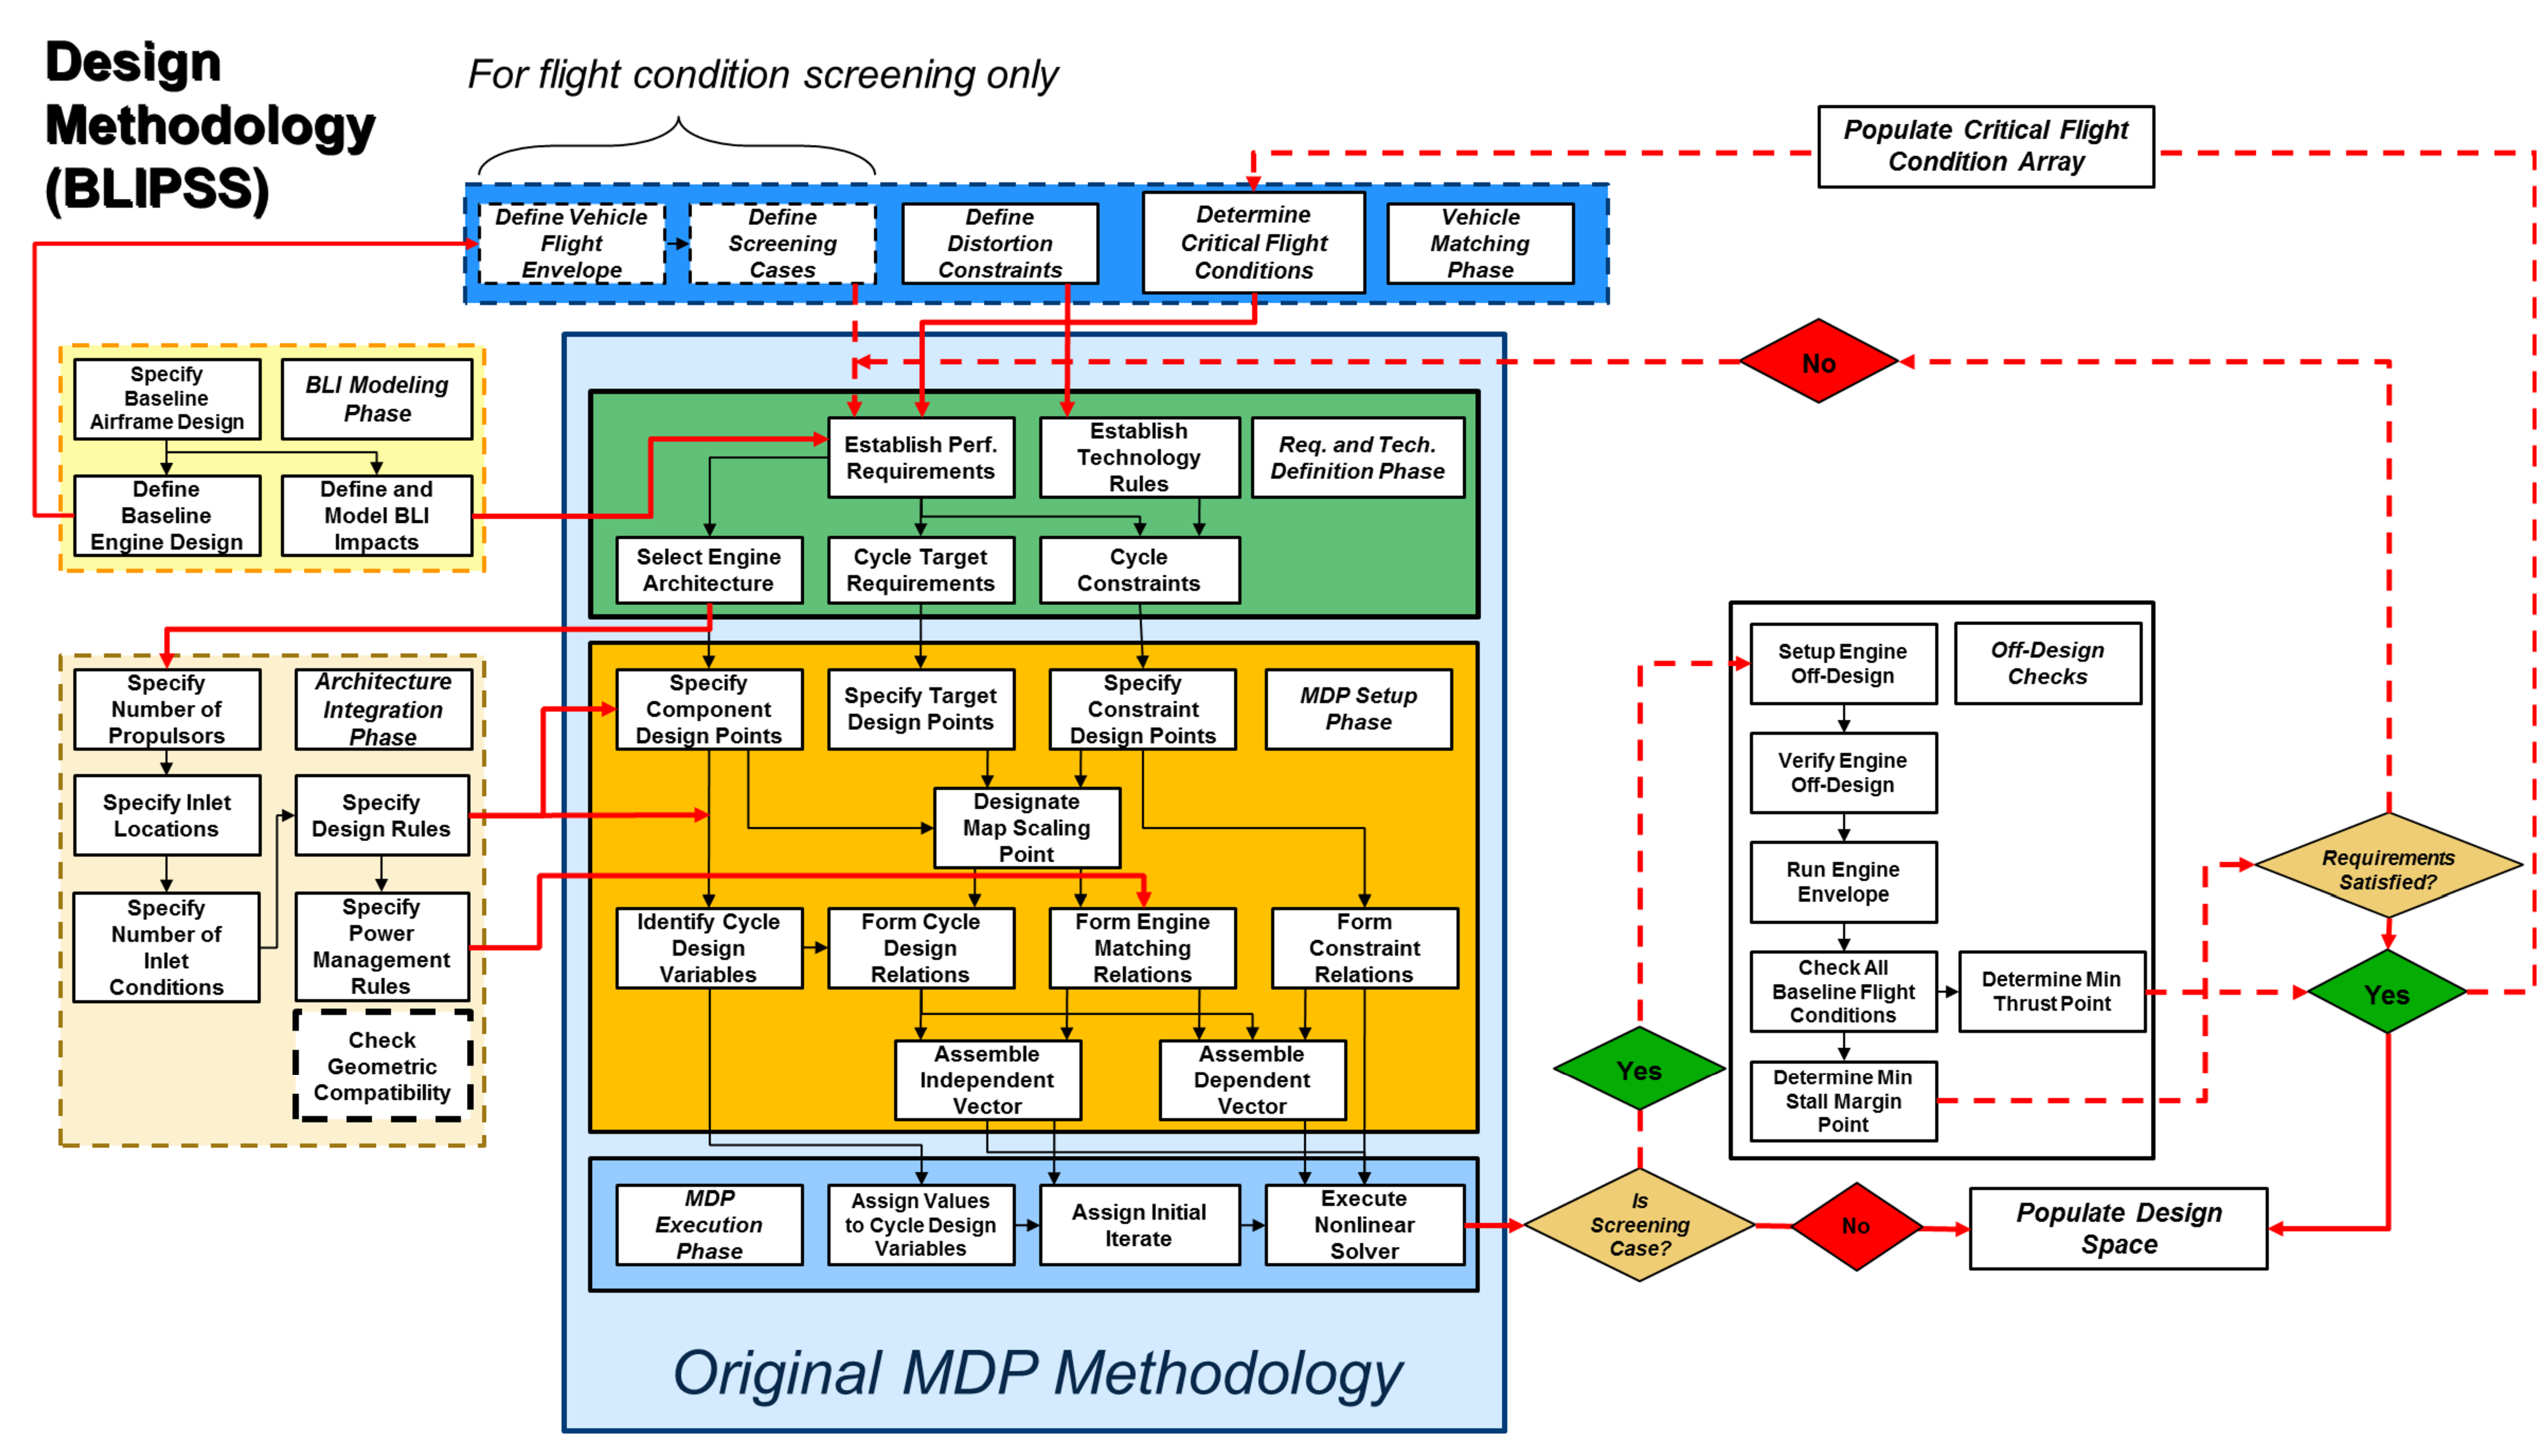
\includegraphics[scale = 0.33, angle = 90]{Design_Methodology.eps}
				\caption{BLIPSS Methodology Data Flow Chart}
				\label{Design_Methodology}
			\end{figure}
			
		\subsection{BLI Modeling Phase Overview}
			The BLI modeling phase is the phase of analysis in which the components of the engine cycle analysis which are impacted by BLI -- in terms of both performance and operability -- are modified to account for these affects.  It is clear that this at least requires the definition of a baseline vehicle and engine for a point comparison.  The baseline engine can either be defined in terms of an already design fixed engine or it could be a competitive architecture, such as a standard podded turbofan engine.  The vehicle definition should be sufficient to define the boundary layer models required in this phase.  This could be given in terms of boundary layer data at necessary flight conditions or vehicle geometry on which analysis is to be conducted in the BLI modeling phase.  
			
		\subsection{Architecture Integration Phase Overview}
			The architecture integration phase is the phase of the analysis in which the particular architecture which is chosen during the requirements and technology definition phase is defined in terms of the number of propulsors and their locations on the vehicle.  The phase requires the specification of a number of propulsors and a location of each propulsor.  From this, the number of unique inlet conditions and propulsors can be determined and a model for each unique propulsor can be defined within the MDP setup phase.  The design strategy choices made during the architecture integration phase affects the number of turbo-machinery design points and the flight conditions which are chosen for them.  The power management strategy are choices made by the designer to determine how different propulsors are power managed.  These choices, as well as the architecture itself, determines the overall engine matching relation for the system, which will be different than for a traditional, single-inlet, MDP setup phase.
						
		\subsection{Vehicle Matching Phase Overview}
			The vehicle matching phase is the phase in which the critical flight conditions for which the system must be sized are determined for the BLIPSS process.  A set of requirements for the distortion constraint must be specified in this phase, along with a series of flight conditions which are to be evaluated.  In order to reduce the run-time of the design study, an initial screening exercise is conducted to determine which flight conditions are most critical.  This is done for a sub-set of the overall design space, and the results are used to determine the most likely flight conditions which will dominate the sizing of the engine.  The flight conditions which are determined to be critical are then included for all non-screening cases going forward within the DoE.  This is done to both limit the amount of cases for which a full off-design check must be done and also limiting the amount of flight conditions which are added to the MDP requirements definitions phase, since adding too many points can make convergence more difficult and also makes programming the MDP process much more difficult.
	\section{Methodology Development:  Research Questions and Hypotheses}		
		\subsection{BLI Modeling Phase}
			The history of the analysis of boundary layer ingesting engines, much as the history of any analysis, is littered with varying levels of modeling fidelity and assumptions with often quite disparate results.  The complicated nature of the question -- viscous and turbulent airframe-propulsion interaction -- often lends itself to convenient simplications for the sake of expediency in order to draw some initial conclusion about potential net benefits and viable configurations.  Once such decisions have been made, engineers are free to move on to the difficult work of determining the validity of the assumptions and analysis via higher order toolsets such as modern Navier-Stokes codes and the like.  This is all very typical of a usual design process, in which conceptual design begins with some crude assumption and is refined by later analysis and optimization.  However, the point of this thesis is to try to get closer to a feasible answer -- at least for the basic propulsion system cycle design and sizing -- before the aerodynamicists embark on refining the assumptions that went into making that decision.  Furthermore, it is intended to guide the aerodynamicist and experimentalist in appropriately directing finite resources for their efforts in the most productive directions (correct flight conditions, configurations, initial geometry, etc), and providing sufficient data back to the propulsion engineer in an iterative process which eventually converges on a solution.  It is with this basic project in mind that research question 1 is formulated and stated simply as follows:
			\vspace{25pt}
			\vspace{5mm}
			\fbox{
				  \parbox{\textwidth}{
						Research Question 1:  What are the minimum requirements for conceptual level modeling of a boundary layer ingesting cycle model in order to reasonably construct the architecture and cycle design space of a BLI propulsion system?
						\vspace{5 mm}
				  }
			}
			\vspace{5mm}
	
			Note that the question asks for the "minimum" modeling requirements for conceptual design.  In a sense, this is asking "what can we get away with" or "what is good enough" at the conceptual level, since obviously the best case scenario is to build a complicated fluid dynamics model, allow it to run on an infinitely powerful computer, and come back with a high-fidelity answer.  Unfortunately, no such computer exists and even if it did, the designer would still have to know which design to model.
			
			In attempting to answer this question, we first take on some components of the answer as being trivial and therefore not worth further investigation; one needs a reasonable engine cycle model to begin with, as well as thermodynamic component models for the constituent machinery and ducting;  one also needs some approximation of the vehicle flow field at the points where it interacts with the engine and a total clean vehicle drag which translates to a thrust requirement.  These are the first few blocks of the "BLI modeling phase" and it is somewhat obvious that they must be known to complete any analysis of the system.  
			
			The component of the question which is far more interesting, however, is in quantifying the interaction between the flow field and propulsion system and its impact on system performance.  These interactions can broadly be classified into 3 regimes: power balance (or thrust balance), turbomachinery performance and efficiency, and engine stability.  The first two have been looked at by almost every author on the subject, while the latter has been studied by some component designers, aerodynamic engineers, and a few others INSERT REFERENCE HERE.  Stability, though it is certainly a dominant concern among technologists, planners INSERT REFERENCE HERE, and experimentalists INSERT REFERENCE HERE, has tended to take a "back seat" at the cycle analysis level, in part because it is a difficult subject to analyze, but also because it is often assumed that modern aerodynamic methods will solve the problem after the fact INSERT REFERENCE HERE.  For this reason, we will begin the analysis by ignoring the stall margin question and returning to it later to analyze this dubious partitioning of the problem.
			
			THE BLIPPS methodology considers the possibility that flight conditions which may normally be analyzed in engine off-design mode might actually be a sizing point required for the MDP on-design analysis.  Therefore, the analysis will also be separated into two different operational modes: engine on-design and off-design.  On-design is the analysis which typically sets the size of the engine, while off-design is any operational condition which deviates from those conditions, including variations in flight Mach number, altitude, or throttle setting ("part power").  On-design analysis essentially sets the level of thrust production and efficiency that the system is capable of providing, while the off-design analysis determines the variation of those quantities over a range of operating conditions including system power setting (mass flow ratio).  It is thus necessary to consider both modes of operation, but we will begin with the subject of engine on-design analysis.	
			
			\subsubsection{\textbf{On Design Analysis with BLI}}
				In order to conduct engine sizing during on-design analysis, it is necessary to augment the basic thrust or power balance relations which match the vehicle requirement with the propulsion system.  For example, the basic textbook thrust equation for a podded engine $F = \dot{m}(U_j - U_\infty)$ must be modified to include the effect of BLI on the system.  The following analysis establishes the basic power balance relations for boundary layer ingesting according to the most current literature, predominantly produced by MIT in theoretical form \cite{Drela2009}.	
		
				We begin with defining the basic power balance equation for any vehicle in an aerodynamic flow which follows from the analysis of Drela:
				\begin{equation}
					P_s + P_v + P_k = W\dot{h}+\dot{E} + \Phi
					\label{Power_Balance}
				\end{equation}% \\
				Here, the term $P_s$ represents the net propulsor shaft power or wing flapping power input to the control volume.  Since here we are only considering the case where the turbomachinery are outside of the CV, the $P_s$ is considered to be 0, and the effect of the work done by the turbomachinery is included in the net flow of propulsor mechanical energy into the CV represented by $P_k$.  The $P_v$ term represents the net pressure-volume power provided by the fluid expanding to atmospheric pressure and can be non-zero in this case, depending on the character of the nozzles.  
				
				\indent The terms on the right hand-side of the equation represent the potential energy change due to climbing ($W\dot{h}$), the total flow-rate of mechanical energy out of the control volume ($\dot{E}$), and the total rate at which kinetic energy is converted into heat inside of the CV ($\Phi$).  The $\dot{E}$ term can be decomposed into various components, but the primary term to consider for subsonic transports of the type considered here is the rate of wake transverse kinetic energy deposition $\dot{E}_v$.  For the case of a relatively close trefftz-plane, where trailing vortices have not dissipated, this term is essentially the equivalent of $V_\infty$ times the induced drag $D_i$ INSERT REFERENCE HERE (Drela).  
		
				\indent The dissipation rate $\Phi$ can be broken down into three components:  surface and wake dissipation due to the presence of the boundary layer, and dissipation in the jet stream aft of the propulsors.  Re-writing Eq. \ref{Power_Balance} according to this decomposition and the assumptions described above, we have the following:
				\begin{equation}
					P_k + P_v = W\dot{h}+\dot{E}_v + \Phi_{surf} + \Phi_{wake} + \Phi_{jet} 
					\label{Power_Balance_Rewrite}
				\end{equation}%
				This equation describes the basic power balance relation for the case of an aircraft with a propulsor whose internal volume is not considered part of the control volume analysis and for the case of a subsonic transport aircraft.  It is valid for both isolated propulsors and the BLI case.  The following sections will describe both of these cases, their differences, and identify key observations from the analysis that are relevant to the research question.
	
				\subsubsection{\textbf{Podded Case}}
					The basic configuration for the podded case -- shown in figure \ref{Podded_Control_Volume} -- illustrates the fact that the propulsor is (at least to first order) separated from the airframe.  Equation \ref{Power_Balance_Rewrite} can therefore be simplified into terms that are more familiar to an aerodynamicist using standard momentum-based techniques.
						\begin{figure}[htp]
							\centering
							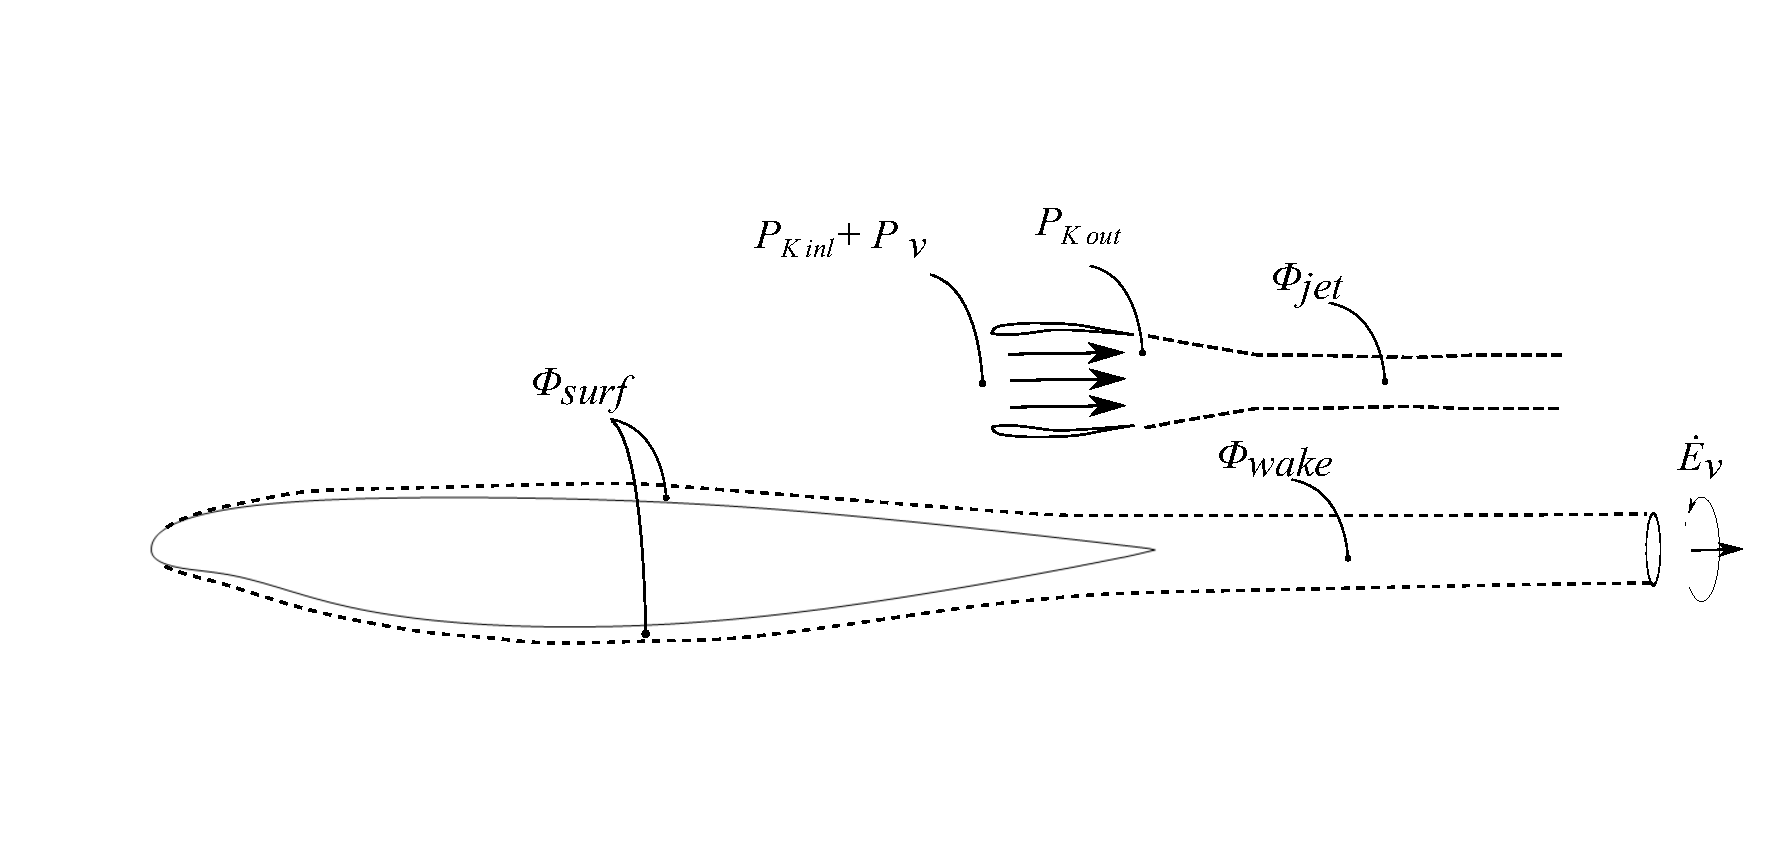
\includegraphics[scale = 0.5]{Podded_Control_Volume.eps}
							\caption{Diagram of the podded case illustrating the various components of the power balance equation.}
							\label{Podded_Control_Volume}
						\end{figure}
					\vspace{15pt}
					\indent First, the drag of the aircraft is normally divided broadly into profile drag (due to friction) and "lift-dependent drag" (due to trailing vortices).  The first is manifested in the dissipation terms ($\Phi_{surf}$ and $\Phi_{wake}$) and is the sum of the surface and wake dissipation, and the second is represented by $\dot{E}_v$.  These power based terms can be translated into an equivalent drag by dividing them by the free-stream velocity $V_\infty$.
					\indent The left-hand side of the equation has to do  with the engine kinetic energy flux into and out of the control volume and the volumetric mechanical power integral $P_v$.  Writing the equation for $P_k$:
					\begin{equation}
						P_k = \oiint{-\big[(p-p_\infty) + \frac{1}{2}\rho(V^2-V_\infty^2)\big]V \cdot \hat{n} dA}
						\label{Pk_Equation}
					\end{equation}%
					Taking this equation and separating out the integral into that over the inlet and exit as shown in figure \ref{Podded_Control_Volume} and also assuming that the nozzle is not significantly over or under expanded ($p \simeq  p_\infty$) gives:
					\begin{equation}
						P_{k_{out}} = \oiint{-\big[\frac{1}{2}\rho(V_j^2-V_\infty^2)\big]V \cdot \hat{n}dA_{nozzle}}
						\label{Pk_Equation_Expanded}
					\end{equation}
					simplifying, we get:
					\begin{equation}
						P_{k_{out}} = \frac{1}{2} F_n (V_j + V_\infty)
						\label{Pk_Equation_Expanded_More}
					\end{equation}
					Where the net thrust, $F_n$ is as normally defined from the simple jet equation.  From the same assumptions as above, 
					\begin{equation}
						P_{k_{inl}} + P_v=0
						\label{Pk_and_Pv}
					\end{equation}
					Now, the dissipation in the jet stream $\Phi_{jet}$ is essentially the wasted kinetic energy of the stream which is eventually converted back into heat after it has been dissipated in the jet.  This can be calculated as follows:
					\begin{equation}
						\begin{aligned}
							\Phi_{jet} = \iint \frac{1}{2}\big(V_\infty - V_j \Big)^2 \rho V_j dA_{nozzle} \\
								      =- \frac{1}{2} F_n \Big(V_\infty-V_j\Big)
						\end{aligned}
						\label{Phi_Jet_Equation}
					\end{equation}
					From \ref{Pk_Equation_Expanded_More} and \ref{Phi_Jet_Equation}, we get:
					\begin{equation}
						P_{k_{out}}-\Phi_{jet}  = V_\infty F_n
						\label{Net_Thrust_Power}
					\end{equation}
					So, the power contribution of the propulsor is essentially the net kinetic energy flux that the propulsor provides to the total aircraft control volume minus the rate at which energy is dissipated in the jet stream wake.  Now that all of the terms of the power balance equation have been defined, we can re-write the equation to be in terms more familiar to the aerodynamicist:
					\begin{equation}
						\begin{aligned}
							V_\infty F_n = W\dot{h} + V_\infty D_i + V_\infty D_p \\
					 		= W\dot{h} + V_\infty D
							\label{Drag_Thrust_Equation}
						\end{aligned}
					\end{equation}
					Other terms, such as an acceleration term or friction forces during ground roll could be added, but this is sufficient for steady-state flight with a constant climb or descent rate.
				\subsubsection{\textbf{BLI Case}}
					The BLI case, illustrated in figure \ref{BLI_Control_Volume}, is clearly different in two ways:  first, there is an inlet defect due to the presence of the boundary layer, such that $P_{k_{inl}}$ is non-zero; second, there is a component of the wake dissipation which is not present since it is ingested into the propulsor and replaced by the jet stream.  The following analysis will develop a mathematical comparison between this case and the original podded case.
					\vspace{-5pt}
					\begin{figure}[htp]
						\centering
						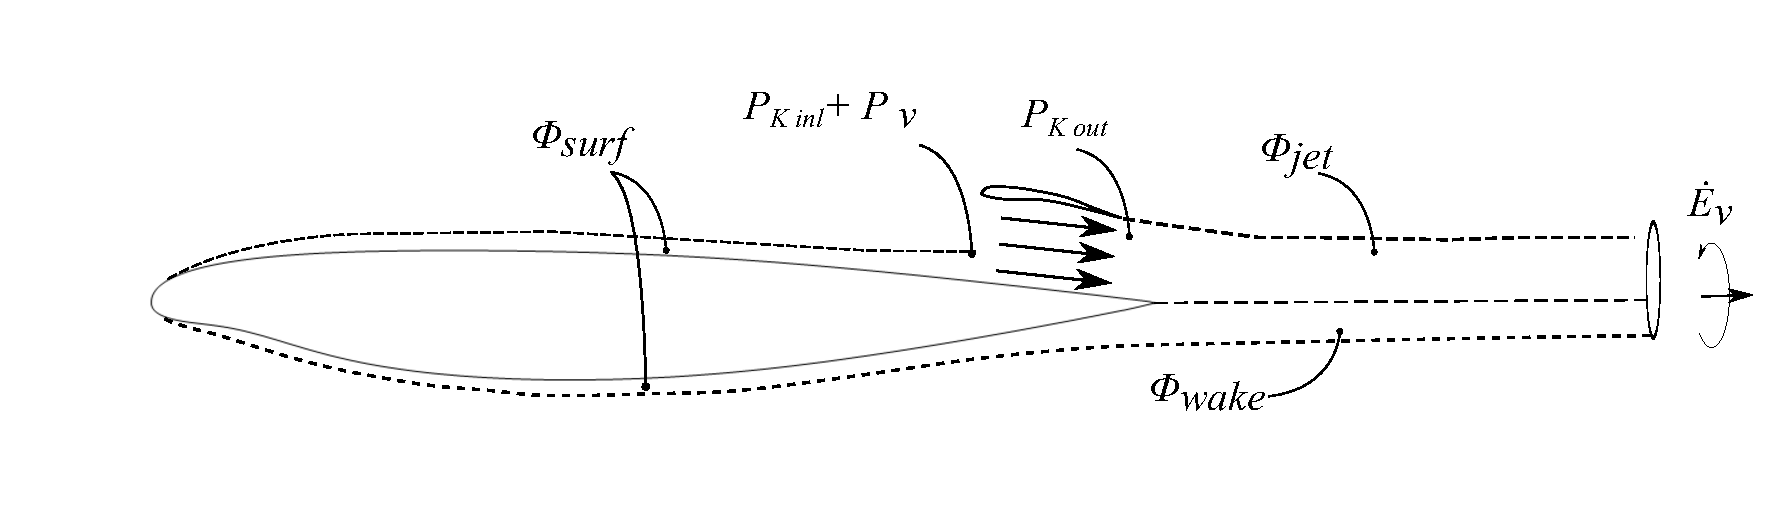
\includegraphics[scale = 0.5, trim = 10mm 10mm 10mm 0mm]{BLI_Control_Volume.eps}
						\caption{Diagram of the BLI case illustrating the various components of the power balance equation.}
						\label{BLI_Control_Volume}
					\end{figure}
					First, it is necessary to define a relationship between the podded (clean vehicle) case and the BLI case.  This is done by defining a parameter $\beta$, which represents the ratio of the wake dissipation in the BLI case to the podded case:
					\begin{equation}
						\Phi_{wake_{BLI}} = (1 - \beta)\Phi_{wake} = (1 - \beta) (\Phi_{\infty}-\Phi_{TE})
						\label{beta_definition}
					\end{equation}
					The inlet defect $P_{k_{inl}}$ is equivalent to the surface dissipation ingested into the propulsor at the inlet location of the propulsor:
					\begin{equation}
						P_{k_{inl}} = \Phi_{Inl} =  \gamma \Phi_{surf} = \gamma \Phi_{TE}
						\label{Inlet_defect_equation}
					\end{equation}
					The parameter $\gamma$ is defined in Eq. \ref{Inlet_defect_equation} as the ratio of the surface defect at the point of ingestion as normalized by the defect in the podded case at the trailing edge.  
					
					In general the surface dissipation is not changed much by the presence of the propulsor, except for the fact that the wetted area of the fuselage upper surface is decreased.  Given the parameters defined above, the following derivation for the surface dissipation in the BLI case is made:
					\begin{equation}
						\Phi_{surf,_{BLI}} = \Phi_{surf} - \beta \Phi_{surf} + \gamma \Phi{surf}
						\label{BLI_Surf_Def}
					\end{equation}
					The assumption being made here is that the proportion of the wake kinetic energy which is recovered is the same as the proportion of the trailing edge dissipation in the BLI case to the total TE (surface) dissipation in the podded case.  Equation \ref{BLI_Surf_Def} then states that the total surface dissipation in the case of BLI is the podded value, minus the trailing edge ingested value, plus the value of the dissipation at the inlet.  Therefore, the term $(\beta - \gamma)$ represents the percent change in the surface dissipation integral.
					\begin{equation}
						\Phi_{surf_{BLI}} = (1 - \beta + \gamma)\Phi_{surf}
						\label{gamma_definition}
					\end{equation}
					 In the case where the propulsor is assumed mounted on the trailing edge of the vehicle, $\gamma$ and $\beta$ are equal and the surface dissipation between the two cases is assumed identical unless the propulsor affects the upstream dissipation in the pre-entry region.  Moving the propulsor far forward would tend $\gamma$ and $P_{k,_{inl}}$ towards zero and would also have an impact on the actual value of $\beta$, as it would be unclear how the jet stream would interact with the surface aerodynamics.  In any case, this would be undesirable and so the case is not considered.
					   
					Finally, we define a similar ratio between the induced drag in the BLI case and the podded case:
					\begin{equation}
						\dot{E}_{v_{BLI}} = \zeta \dot{E}_{v}
					\end{equation}
					The above definitions can be used in conjunction with Eq. \ref{Power_Balance} to write the final power balance equation for the BLI case:
					\begin{equation}
						(P_{k_{out}} - \Phi_{jet}) + \gamma \Phi_{surf} = (1 - \beta + \gamma) \Phi_{surf} + (1-\beta) \Phi_{wake} + \zeta \dot{E}_v + W\dot{h}
						\label{BLI_Power_Balance}
					\end{equation}
					Rearranging and simplifying:
					\begin{equation}
						(P_{k_{out}} - \Phi_{jet}) + \beta (\Phi_{surf} + \Phi_{wake}) = \Phi_{surf}+\Phi_{wake} + \zeta \dot{E}_v + W\dot{h}
						\label{BLI_Power_Balance_Simplified}
					\end{equation}
					Using the results from the podded analysis, we get:
					\begin{equation}
						\underbrace{\strut V_\infty F_n  + \beta \Phi - \zeta \dot{E}_v}_{\text{Total Net Thrust}} = \underbrace{\strut V_\infty D + W\dot{h}}_{\text{Podded Vehicle Drag}}
						\label{Podded_Power_Balance_Final}
					\end{equation}
					
					Here, the term $\beta$ represents all changes to the viscous wake profile in relation to the podded case for an aft-mounted propulsor.  This includes the recovery of the wake dissipation, which is now replaced with the jet stream, and another term that essentially represents a reduction in the flux of kinetic energy into the propulsor control volume (ram drag reduction).  This equation is generally simplified, at this level of analysis, by assuming that $\zeta$ is also zero and therefore the vortex drag is not altered in the case of BLI.  We will see in later sections that this is most likely an inappropriate assumption for very high or low engine power levels, where the surface static pressure distribution is modified significantly by the pre-entry flow.  This creates an awkward scenario where the actual drag polar, lift, and pitching moment of the vehicle would be throttle dependent, totally throwing asunder all notions of the book-keeping separability of thrust and drag.  At the level of conceptual design and cycle analysis, it is essentially necessary to ignore the effect of the engine on the lift distribution since to model this would be cumbersome and is unlikely to have much effect on the sizing of the engine, which is typically done at normal power levels where pre-entry flow pressure gradients are small.  																	 
					
				\subsubsection{Performance Parameters}
					It is now useful to define some performance parameters based on this analysis to determine how this might affect the system in relation to the podded case. The thrust saving coefficient is defined as the proportion of the total net thrust of the propulsor which is related to the BLI wake-recovery effect.  
					\begin{equation}
						TSC = \frac{\beta \cdot \Phi}{\Big(V_\infty F_n  + \beta \Phi - \zeta \dot{E}_v \Big)} = 
						\frac{\beta \cdot \Phi}{\Big(V_\infty D + W\dot{h} \Big)} 
						\label{Thrust_Saving_Coefficient}
					\end{equation}
					Where again, $F_n$ is defined as above.  At times, others define the slightly less useful parameter (\%BLI) is used and defined as the ratio of the wake recovery term to the total drag (ratio of ingested drag to uningested drag).  Assuming that $\zeta$ is zero and that there is no excess power required for climb or acceleration, the thrust saving coefficient and \%BLI are the same for the vehicle as a whole.  																									

					The "BLI" efficiency was defined by Sato INSERT REFERENCE HERE and includes the contribution from both the wake recovery and the propulsive efficiency increase of the engine due to the kinetic energy defect at its inlet.					
					\begin{equation}
						\eta_{_{BLI}} = \frac{\Big(T \cdot V_\infty\Big)_{Podded}}{\Big(\Delta KE\Big)_{BLI}} = C_{BLI} \cdot \eta_{pr_{BLI}}
						\label{eta_BLI}
					\end{equation}
					With $C_{_{BLI}}$ defined as the ratio of the dissipation and vortex loss terms (rhs of power balance):
					\begin{equation}
						C_{BLI} = \frac{\dot{E_v}+\Phi}{\dot{E_v} + (1-\beta)\Phi + \gamma \Phi_{surf}}
					\end{equation}
					$C_{BLI}$ is generally greater than unity for non-zero BLI so that is has the effect of increasing the overall value of $\eta_{BLI}$.  Higher values of $\beta$ obviously tend to give more benefit.  
					
					The propulsive efficiency for a BLI propulsor is calculated according to its definition:
					\begin{equation}
						\eta_{pr} = \frac{P_k - \Phi_{jet}}{P_k} = \frac{P_{k,_{out}} - \Phi_{jet} + P_{k,_{inl}}}{P_{k,_{out}} + P_{k,_{inl}}}
						\label{Propulsive_Efficiency}
					\end{equation}
					This can be rewritten by using Eq. \ref{Inlet_defect_equation} to compute the inlet defect.  
					\begin{equation}
						\eta_{pr} = \frac{P_{k,_{out}} - \Phi_{jet} + \gamma \Phi_{surf}}{P_{k,_{out}} +\gamma \Phi_{surf}}
						\label{Propulsive_Efficiency_Rewritten}
					\end{equation}
					In the case of no BLI (no $P_{k,_{inl}}$), then Eq. \ref{Propulsive_Efficiency_Rewritten} simplifies to the normal Froude propulsive efficiency equation.  With ($\gamma > 0$), $\eta_{pr,_{BLI}} > \eta_{pr,_{Podded}}$, meaning there is a propulsive efficiency benefit for ingesting BLI, along with the general reduction in the amount of power required to propel the aircraft (represented by $C_{BLI}$).  
					
					The overall efficiency of the podded (non-BLI) propulsion system is defined as follows:
					\begin{equation} 
						\eta_o = \frac{F_n \cdot V_\infty}{\dot{m}_f \cdot h_{LHV}} = \frac{V_\infty}{TSFC \cdot h_{lhv}}
						\label{Overall_Efficiency}
					\end{equation}	
					For the BLI case, 
					\begin{equation}
						\eta_o = \underbrace{\Big[\frac{\Big(F_n \cdot V_\infty\Big)_{Podded}}{\Big(F_n \cdot V_\infty\Big)_{BLI}}\Big]}_{\text C_{BLI}}
								 \underbrace{\Big[\frac{\Big(F_n \cdot V_\infty\Big)_{BLI}}{\Big(\Delta KE\Big)_{BLI}}\Big]}_{\text Prop. Efficiency}
						         \underbrace{\Big[\frac{\Big(\Delta KE\Big)_{BLI}}{\Big(\dot{m}_f \cdot h_{lhv}\Big)}\Big]}_{\text Thermal. Efficiency}								 
					\end{equation}									
					
					Therefore, the benefit is seen to be a function of two phenomena:  1.) the reduction in the wake dissipation which is no longer present; 2.) An increase in the propulsive efficiency because of the non-zero kinetic energy defect entering the propulsor (ram drag reduction).  Both of these are also found to be strong functions of the amount of BLI ingested, with the final power balance being mainly a function of $\beta$.  This standard observation from the BLI literature is therefore formulated as follows:
															
					\vspace{1pt}
					\vspace{5mm}
					\noindent{
						\fbox{
					  		\parbox{\textwidth}{
										\textbf{Observation 1}:  The performance benefit of boundary layer ingestion systems is generally a function of the ratio of the amount of equivalent viscous drag ingested by the propulsor to the total drag in the podded case.
					  					}
							}
					}
					
					Finally, the use of the thrust saving coefficient can combine the above effects into the thrust specific fuel consumption variable:
					\begin{equation}
						TSFC = \frac{\dot{m}_f \cdot (1-TSC)}{F_n}
						\label{TSFC_Equation}
					\end{equation}
					Changes in propulsive efficiency are then wrapped up into the calculation of the thrust saving coefficient and any changes in thermal efficiency would arise from the calculation of the fuel flow $\dot{m}_f$ from the thermodynamic cycle model.  For this reason, the modified TSFC metric described in Eq. \ref{TSFC_Equation} will be used to describe the benefit of the system going forward.
					
				\subsubsection{Calculation of BLI Benefit}					
					Now that the basic power balance equations for a vehicle with BLI have been established as well as the important parameters contributing to the overall benefit of the system, it is now necessary to define how these quantities can, in theory, be computed.  First, some useful boundary layer quantities are defined INSERT REFERENCE SATO:	\\			
					\textbf{Mass Defect:}						
						\begin{equation}
							\textbf{M} \equiv \rho_e u_e \delta^* = \int \limits_{0}^{\delta}\Big(\rho_e u_e - \rho u \Big)dy
							\label{M_Definition}
						\end{equation}						
					\textbf{Momentum Defect:}
						\begin{equation}
							\textbf{P} \equiv \rho_e u_e^2 \theta = \int \limits_{0}^{\delta}\Big(u_e-u\Big)\rho u \hspace{1mm} dy
						\end{equation}					
					\textbf{Kinetic Energy Defect:}
						\begin{equation}
							\textbf{K} \equiv \frac{1}{2}\rho_e u_e^3 \theta^* = \frac{1}{2} \int \limits_{0}^{\delta}\Big(u_e^2-u^2\Big)\rho u \hspace{1mm} dy
						\end{equation}										
					\textbf{Density-flux Defect:}
						\begin{equation}
							\textbf{D} \equiv \rho_e u_e \Delta^{**} = \int \limits_{0}^{\delta}\Big(\rho_e - \rho \Big) u \hspace{1mm} dy
						\end{equation}					
					The above equations relate the conditions in the boundary flow gradient region to the external inviscid flow (EIF) integrated in the ``y-direction'' normal to the wall.  Note that in the case of turbulence, the definitions above apply only to the mean (time-averaged) quantities but the notation is kept the same for convenience and any reference to a flow-field quantity is referring to the mean value.
					
					Sato INSERT REFERENCE HERE gives a derivation for the evolution of the kinetic energy defect in relation to the profile mechanical loss coefficient $\Phi_p$ shown in Eq. \ref{Defect_Integral_Equation}.  This is effectively conservation of energy in integral form:				
					\begin{equation}
						\int_{out} \textbf{K} \cdot \hat{n} \hspace{1mm} dl_{out} = \Phi_p - \Pi_V
						\label{Defect_Integral_Equation}
					\end{equation}
					
					The above equation is valid for a control volume which has its inlet and side planes sufficiently far from the vehicle such that the integral of the kinetic energy deficit is zero and the ``\emph{out}'' plane is the location of the exiting plane which can be placed at some axial location along the aerodynamic body.  The first term on the right-hand side of Eq. \ref{Defect_Integral_Equation} is the viscous dissipation term:
					\begin{equation}
						\Phi_p = \iint \emph{D} \hspace{1mm} d\emph{S} = \iint \rho_e u_e^3 c_{_D} \hspace{1mm} d\emph{S}
						\label{Viscous_Dissipation}
					\end{equation}					
  				    The second term is the so-called ``baroclinic'' term (Eq. \ref{Baroclinic_Term}), which represents the change in mechanical energy flux due to the pressure gradient acting on the boundary layer flow at a different density than the inviscid flow.  The value of this typically scales with $M_e^2$ and is approximately 5\% for high subsonic flows INSERT REFERENCE HERE.
  				    \begin{equation}
	  				    \Pi_V = \iint \textbf{D} \cdot \bigtriangledown \frac{1}{2} u_e^2 \hspace{1mm} d \emph{S} =  \iint \textbf{D} \cdot u_e \frac{\partial u_e}{\partial x}d\emph{S}
	  				    \label{Baroclinic_Term}
  				    \end{equation}
					
					Placing this plane far down-stream of the body at the Treftz plane ($A_\infty$), the total mechanical dissipation coefficient is given in equation \ref{Treftz_Integral} and represents the total dissipative profile drag for the body on the right hand side of the general power balance (Eq. \ref{Power_Balance}):
					\begin{equation}
						\Phi_p^* = \int_{A_\infty} \textbf{K} \cdot \hat{n} \hspace{1mm} dl_{out} = \Phi_p - \Pi_V
						\label{Treftz_Integral}
					\end{equation}										
					The dissipation term from the power balance equation is then computed by integrating the axial 2-D kinetic energy defect \textbf{K} over the exit plane area.  We now consider this integral for two types of aerodynamic wake profiles.
					
				\subsubsection{``Class 1'' Aerodynamic Body}
					There are two fundamental aerodynamic body shapes, as defined by Kulfan INSERT REFERENCE HERE.  The first is type ``Class 1'', which represents wing airfoil type shapes with a distribution along a stacking axis (Fig. \ref{Class_One_Geometry_Diagram}).  Something like a hybrid wing body design falls into this class of aerodynamic bodies.  					
					\begin{figure}[htp]
						\centering
						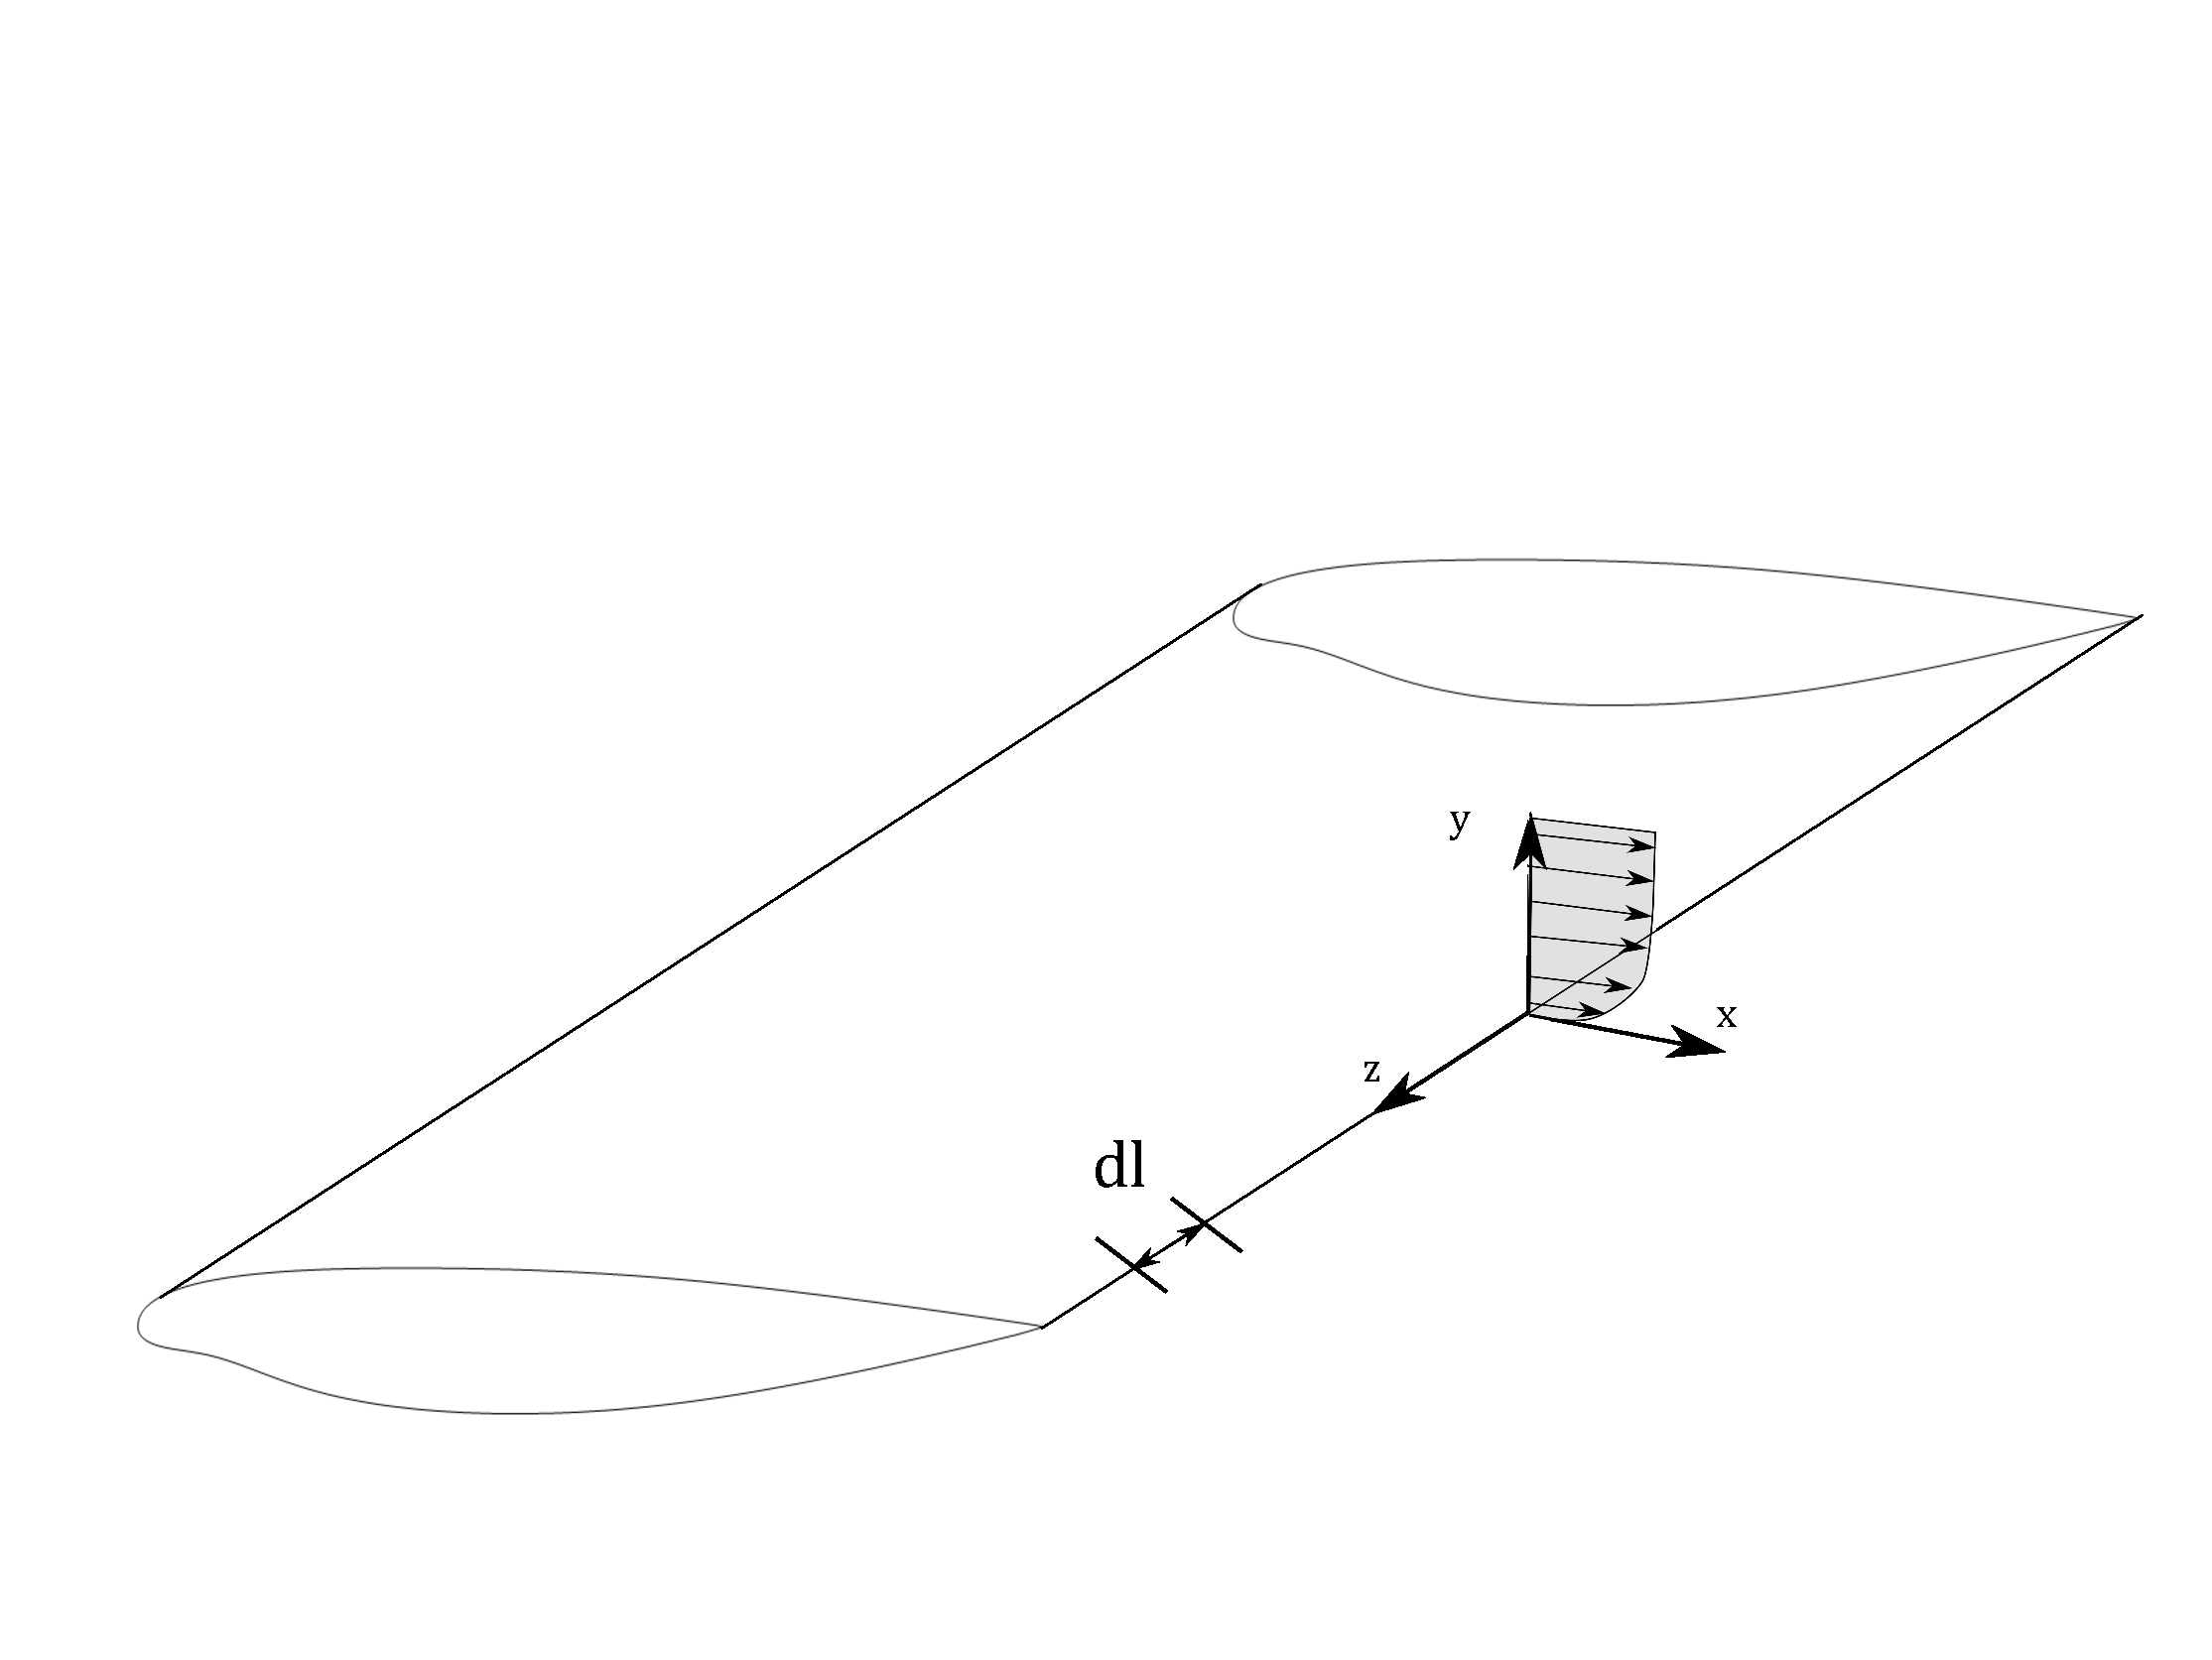
\includegraphics[scale = 0.35, trim = 25mm 30mm 25mm 100mm]{Class_One_Geometry_Diagram.eps}
						\caption{Diagram of a class 1 geometry type with trailing edge boundary layer shown.  The dissipation integral is performed along the z-direction.}
						\label{Class_One_Geometry_Diagram}
					\end{figure}									
					\begin{figure}[htp]
						\centering
						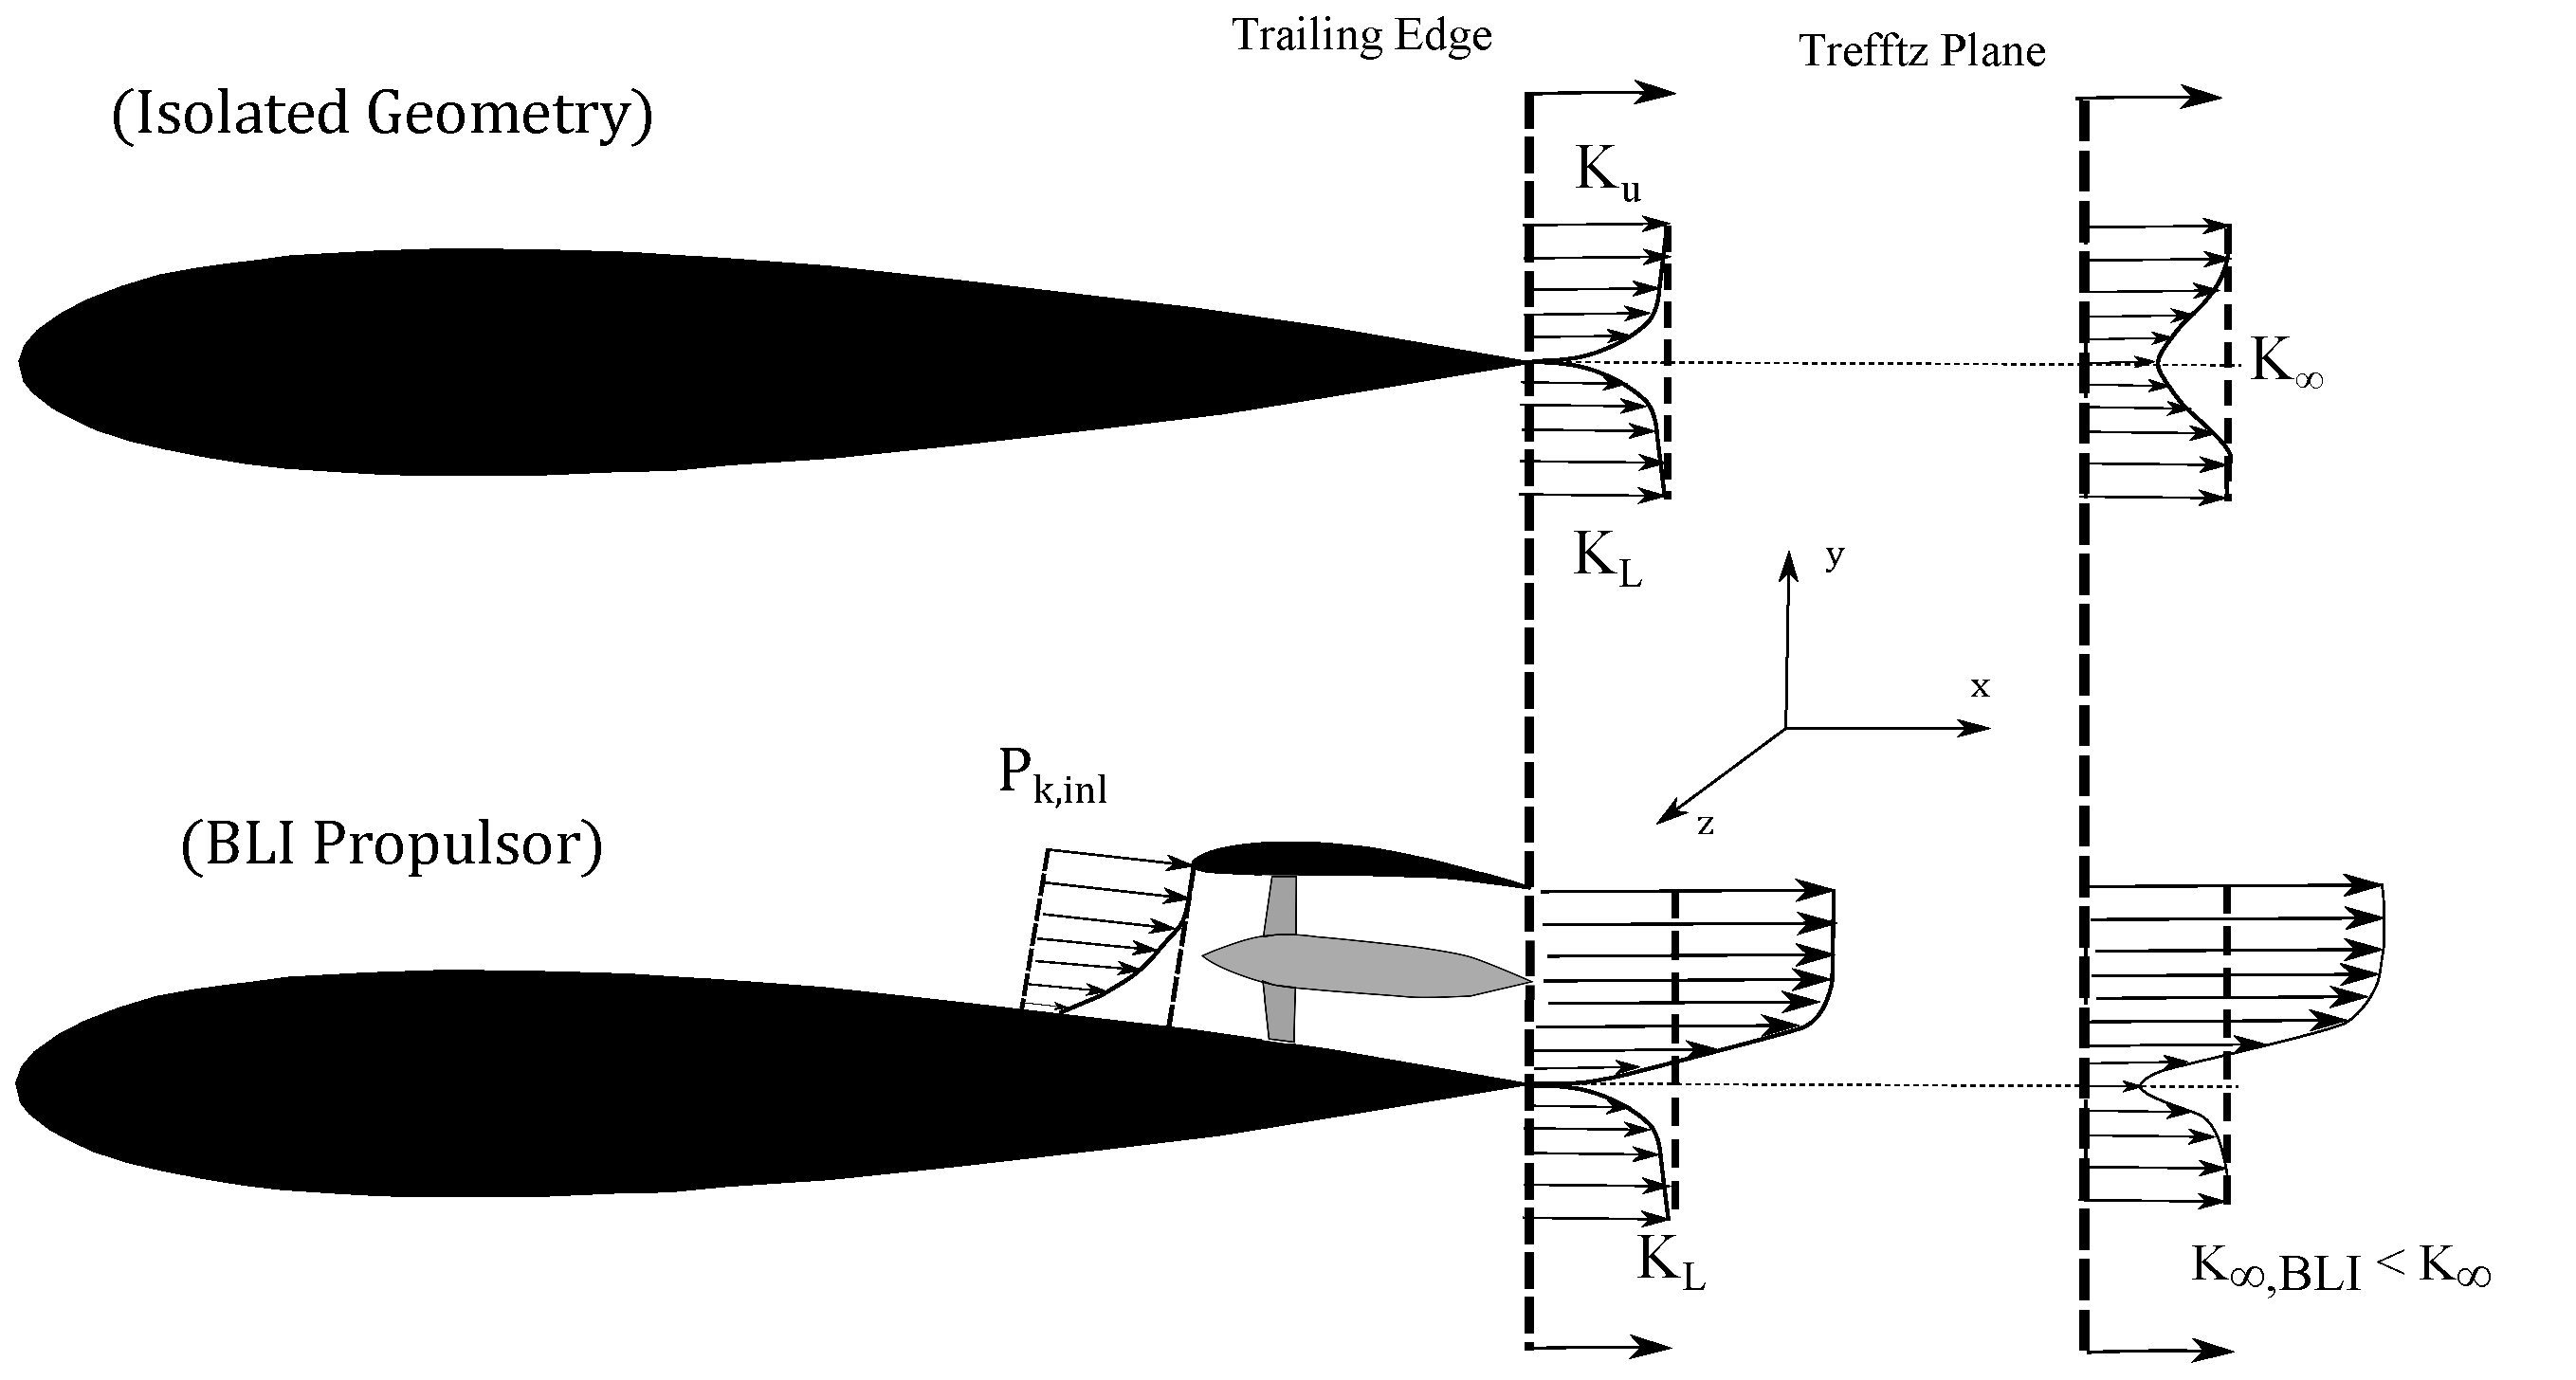
\includegraphics[scale = 0.35]{Class_One_Wake_Diagram.eps}
						\caption{Illustration of a class 1 geometry aerodynamic wake for the isolated airfoil and case with a BLI propulsor.}
						\label{Class_One_Wake_Diagram}
					\end{figure}
					Fig. \ref{Class_One_Wake_Diagram} illustrates the type of wake which develops for a BLI propulsor on a class 1 type aerodynamic body.  The wake dissipation factor for the isolated geometry case is:
					\begin{equation}
					\Phi_p^* = \int K_\infty \cdot \hat{n} \hspace{1mm} dl  = \int \underbrace{\strut (K_L + K_u)}_{\text{Trailing Edge}} \hspace{5mm} + \underbrace{\strut \Phi_{wake}^*}_{\text{Wake dissipation}}
					\end{equation}					
					The wake for the ingesting propulsor case is $K_{\infty,_{BLI}}$ and the parameter $\nu = K_{\infty,_{BLI}}/K_\infty$ is defined to form a relation between the BLI and isolated case.  For $\nu = 1$, there is no boundary layer ingested at that z-location, while $\nu = 0$ represents the case where all of the defect is ingested (lower and upper surface).  An approximation for $\nu$ can be made by assuming that only the contribution of the upper portion of the wake is removed:
					\begin{equation}
						\Phi_{p,_{BLI}}^* = \int \nu \textbf{K}_{\infty} \cdot \hat{n} \hspace{1mm} dl= \int \frac{K_L}{\Big(K_L + K_u\Big)}_{TE} \cdot \Big(\textbf{K}_\infty \cdot \hat{n}\Big) \hspace{1mm} dl
						\label{Phi_P_Star}
					\end{equation} 
					The next step is to carry out the integration over the length of the wake at the trefftz plane to compute the mechanical energy flux for the BLI case in relation to the isolated body case.  Fig. \ref{Kz_Distribution} shows an example ``Class 1'' body with constant cross section and chord length.
					\begin{figure}[htp]
						\centering
						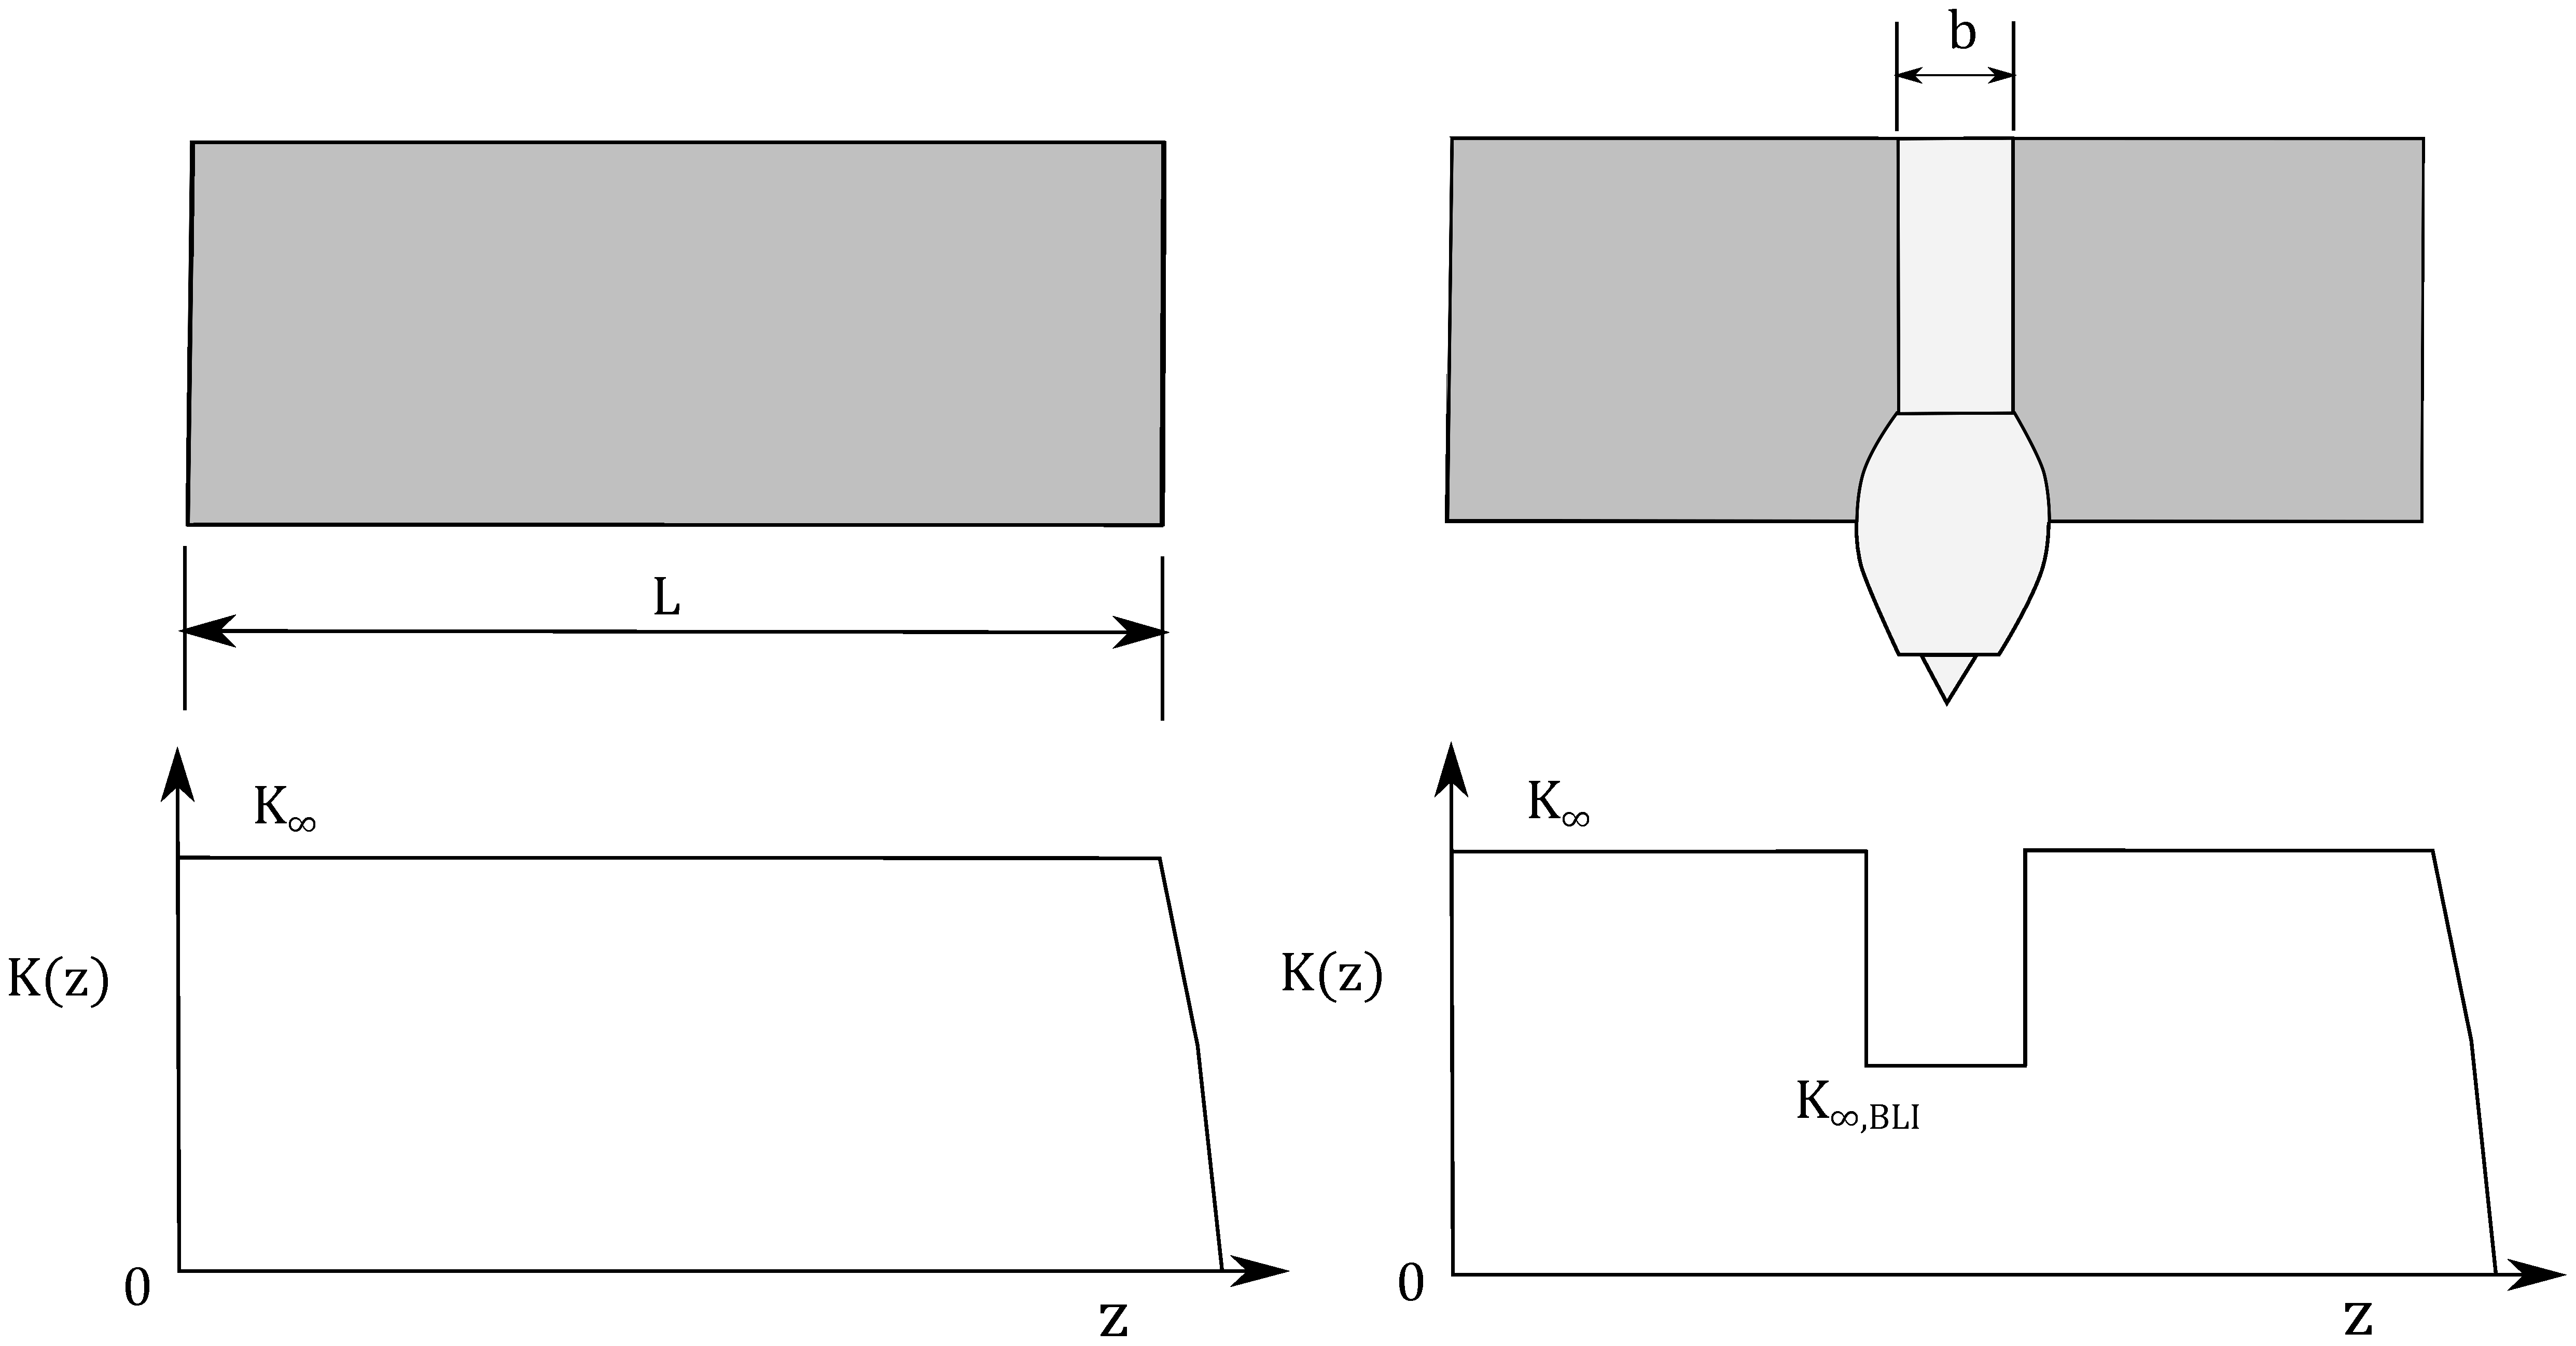
\includegraphics[scale = 0.15]{Kz_Distribution.eps}
						\caption{Illustration of the distribution of the kinetic energy defect over the length of a notional ``class 1'' aerodynamic body.}
						\label{Kz_Distribution}
					\end{figure}															
																														
					The variable "b" here is a term representing the "span", or width, of the ingested boundary layer.  The dissipation integral (Eq. \ref{Phi_P_Star}) is the area under the curve of this distribution.  From this, and by using the definition of $\beta$ in Eq. \ref{beta_definition}, we get the following general relation for a class 1 vehicle:
					\begin{equation}
						1 - \beta = \frac{\Phi_{p,_{BLI}}^*}{\Phi_p^*} = {\displaystyle\int_{x = \infty} \nu(z) K_\infty(z) \hspace{1mm} dz \over \displaystyle\int_{x = \infty} K_\infty(z) \hspace{1mm} dz}
						\label{Beta_Calculation_General}
					\end{equation}
					From fig. \ref{Kz_Distribution}, and carrying out the integration for this notional class 1 body, an approximation of $\beta$ is thus:
					\begin{equation}
						\begin{aligned}
							1 - \beta = \frac{ \Phi_{p,_{BLI}}^*}{\Phi_p^*} = \frac{K_\infty \Big(L-b\Big) + b \nu K_\infty}{LK_\infty} \\%						
								  = \Big(1 - (1-\nu)\frac{b}{L}\Big)
						\end{aligned}
						\label{Beta_Calculation_Specific}
					\end{equation}
					Again, Eq. \ref{Beta_Calculation_Specific} is an approximation, but is at least useful for simple cases and understanding the overall parameters involved in the analysis for the class 1 type.  From Eq. \ref{Beta_Calculation_Specific}, the relationship for the thrust saving coefficient is as follows:
					\begin{equation}
						TSC = \frac{\beta \cdot \Phi_p^*}{DV_\infty + W\dot{h}} = \frac{(1-\nu) b K_\infty}{DV_\infty + W\dot{h}}
						\label{TSC_Class2}
					\end{equation} 
					
					\vspace{1pt}
					\vspace{5mm}
					\noindent{
						\fbox{
					 		  \parbox{\textwidth}{
							  				\textbf{Observation 2}:  For class 1 aerodynamic bodies with BLI, the ratio of ingested drag to net thrust depends on both the value of the recovered boundary layer kinetic energy defect at the trefftz plane and the total span of the boundary layer defect ingested by the engine stream-tube.
					  					   }
							}
					}
					
				\subsubsection{``Class 2'' Aerodynamic Body}
					The ``class 2'' aerodynamic body, as defined by Kulfan INSERT REFERENCE, is the type where the cross-sectional stacking axis is along the ``x-axis''.  These types of bodies are generally things like fuselages, nacelles, missile or payload pods, etc.  These can generally be specified by either having a set of cross-sections which are rotated around some center-line axis or can also be represented by stacking along a vehicle station-line.  For BLI, the important aspect of the class 2 type problem is that the trailing edge and downstream wakes are of a fundamentally different character.  An illustration of this is shown in fig. \ref{Class_Two_Geometry_Diagram} with a notional tube and wing aircraft.  The fuselage tail-cone has a wake at the trailing edge of the vehicle with a circumferential distribution around the body which is roughly uniform.  The gradient in the boundary layer is in the radial or ``y'' direction.
					\begin{figure}[htp]
						\centering
						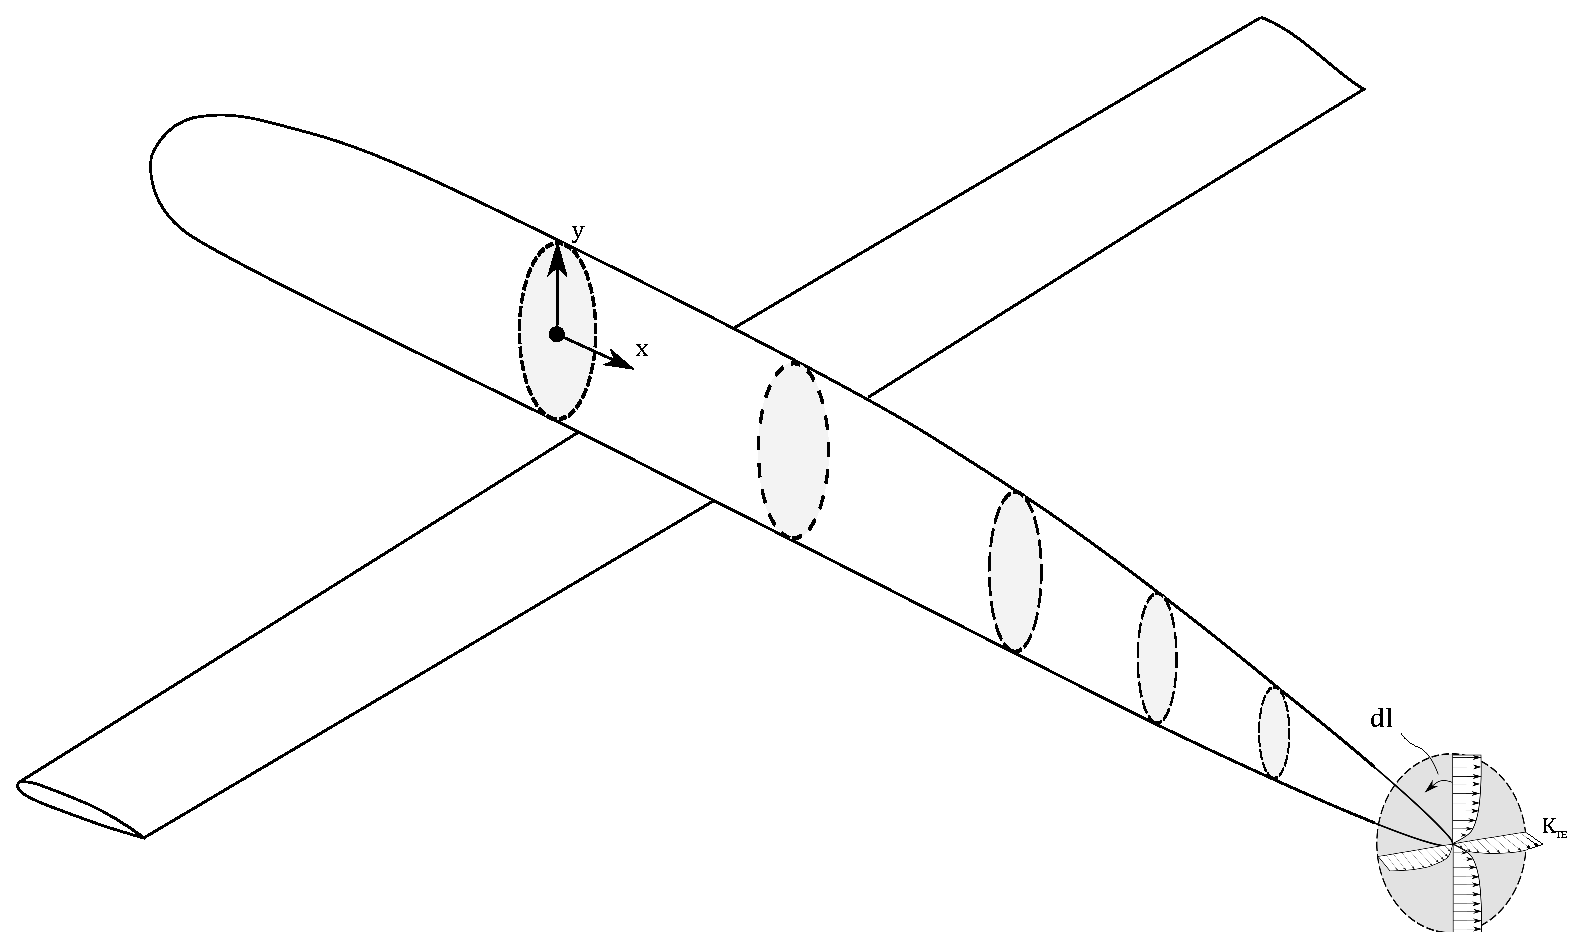
\includegraphics[scale = 0.45, trim = 10mm 0mm 0mm 0mm]{Class_Two_Geometry_Diagram.eps}
						\caption{Illustration of the distribution of the kinetic energy defect over the length of a notional ``class 1'' aerodynamic body.}
						\label{Class_Two_Geometry_Diagram}
					\end{figure}
					
					The wake integral from equation \ref{Treftz_Integral} can be computed by integrating the boundary layer kinetic energy defect over the circumference of the wake and assuming $dl = \delta d\theta$, where $\delta$ is the boundary layer thickness (distance from wall to ``edge'').
					\begin{equation}
						\Phi_p^* = \int_{_{Trefftz}} K_\infty(\theta) \hspace{1mm} \delta \hspace{1mm} d\theta
					\end{equation}
					and the equation for $\beta$, similar to Eq. \ref{Beta_Calculation_General}, is the following:
					\begin{equation}
						1 - \beta = \frac{\displaystyle \int_0^{2\pi} K_\infty (\theta)\hspace{1mm} \nu(\theta) \hspace{1mm}\delta(\theta) \hspace{1mm} d\theta}
										 {\displaystyle \int_0^{2\pi} K_\infty(\theta) \hspace{1mm}\delta (\theta) \hspace{1mm}\hspace{1mm} d\theta}
						 \label{eq:Class2_Beta_Equation}
					\end{equation}
					
					If we assume circumferential uniformity, then the $K_\infty$ and $\delta$ can be pulled out of the integration.  The BLI benefit term ($\beta$), then, is only a function of the fraction ($\nu$) of the isolated wake which is recovered in the BLI case.  For most aerodynamic bodies of practical concern, the wake will be small enough to entirely ingest it inside of an aft mounted propulsor so that $\nu(\theta) = 0$ at every $\theta$ and the wake is entirely recovered, as shown in fig. \ref{Class_Two_Wake_Diagram}.  With $\nu$ everywhere zero at the trefftz plane, then $\beta$ is precisely equal to one, unless the wake from other bodies, such as a wing, is included.  							
					\begin{figure}[htp]
						\centering
						\vspace{5mm}
						
\includegraphics[scale = 0.45, trim = 0mm 0mm 0mm 0mm]{Class_Two_Wake_Diagram.eps}
						\caption{Illustration of the the wake defect for a class 2 body with BLI.}
						\label{Class_Two_Wake_Diagram}
					\end{figure}
					It is likely that the entire wake will not be recovered, as illustrated in fig. \ref{Class_Two_Wake_Diagram}, and that there will be some residual kinetic energy defect in the jet stream of the BLI propulsor.  This can be captured either by modeling the jet stream with an overall gross-thrust coefficient or by including a recovery factor, such as that defined by Smith INSERT REFERENCE HERE, and include the defect in the calculation of $P_{k,{out}}$ in the power balance equation (Eq. \ref{BLI_Power_Balance_Simplified}).  These approaches are equivalent assuming the nozzle gross thrust coefficient is calculated accordingly.
					
					The primary difference between the ``Class 1'' and ``Class 2'' type vehicle with boundary layer ingestion is that a single propulsor can be designed to ingest the entire trailing edge wake defect for the class 2 designs.  As such, observation 2 does not apply for these types of designs.  Furthermore, if the entire wake is ingested by a propulsor which surrounds a class 2 type body, then the distortion will be primarily radial, rather than being a combined radial/circumferential complex distortion profile. This leads to a natural classification for BLI propulsion systems:
					
					\begin{itemize}
						\item{Class 1 BLI Systems:  Laterally distributed boundary layer, for which the calculation of the dissipation integral (wake recovery term) is dependent on the width of the engine ingested stream-tube.}
						
						\item{Class 2 BLI Systems:  Circumferentially distributed boundary layer, for which the dissipation integral is not dependent on the width of the ingested stream-tube, but only on the radius.}
					\end{itemize}
					 					
				\subsubsection{Propulsor Sizing:  Class 1 BLI}	
					Consider the case of a general cross-section with area ``A'' (fig. \ref{General_Cross_Section}) with some velocity distribution over its surface.  The general equation for the mass flux through this cross section is from Eq. \ref{General_Mdot}.
					\begin{figure}[htp]
						\centering
						\vspace{0mm}
						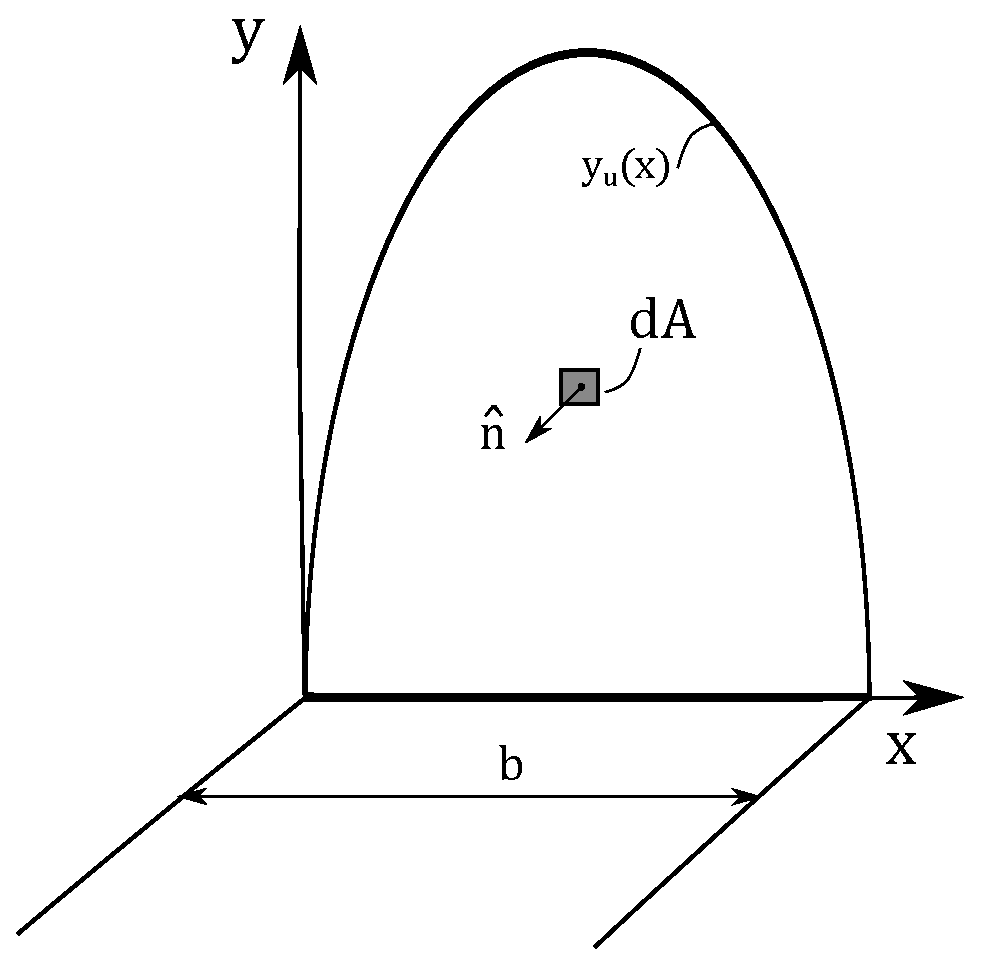
\includegraphics[scale = 0.45, trim = 0mm 0mm 0mm 0mm]{General_Cross_Section.eps}
						\caption{General cross-section diagram.}
						\label{General_Cross_Section}
					\end{figure}					
					\begin{equation}
						\dot{m} = \iint_A \rho (\textbf{u} \cdot \hat{n}) \hspace{1mm} dA = \int_{0}^{b}\int_{0}^{y_u(x)} \rho u_x \hspace{1mm} dy dx
						\label{General_Mdot}
					\end{equation}	
					From Eq. \ref{M_Definition}, 
					\begin{equation}
						\int \rho u \hspace{1mm} dy = \int \rho_e u_e dy - \textbf{M}
					\end{equation}					
					Then:
					\begin{equation}
						\begin{aligned}
							\dot{m} = \int_0^b \Big[\rho_e u_e y_u(x) - \textbf{M(x)}\Big] \hspace{1mm} dx \\
									= \int_0^b \rho_e u_e \Big(y_u(x) - \delta^*(x)\Big) \hspace{1mm} dx
						\end{aligned}
						\label{General_Mass_Sizing}
					\end{equation}
					Here, the edge velocity and density are set by the incoming local properties which are a function of the vehicle aerodynamic shape and free-stream conditions.  Therefore, if the designer desires a specified mass flow, then the width or height of the inlet can be adjusted to achieve the desired mass flow, and the integration of Eq. \ref{General_Mass_Sizing} is computed to do so.  If the cross-section shape is known (fixed b and h), the mass flow through that cross-section can be calculated from this relation.  To demonstrate this in a simple way, the assumption is made that the 1-D mass defect $\delta^*$ and edge velocity and density are constant in the x-direction over the length of the inlet.  From this assumption, 					
					\begin{equation}
						\dot{m} = \rho_e u_e \int_0^b y_u(x) \hspace{1mm} dx - \rho_e u_e \delta^* b
						\label{Simplified_Mass}
					\end{equation}
					Defining $h = max(y(x))$, and recognizing that $\int y(x)dx = A$, the following definition is useful:
					\begin{equation}
						r^* = \frac{\displaystyle A}{b \cdot h}
					\end{equation}
					Here, $r^*$ is a measure of how closely the inlet shape matches to a rectangular shape, with a value of unity representing a rectangle with width ``b'' and height ``h''.  Defining the inlet aspect ratio to be $AR = b / h$, then Eq. \ref{Simplified_Mass} becomes:
					\begin{equation}
						\dot{m} = \rho_e u_e \hspace{1mm} \hspace{1mm} \frac{r^* b^2}{AR} \hspace{1mm} - \rho_e u_e \delta^* b
					\end{equation}
											
					Then, the above quadratic equation can be solved for the cross-section width, which directly multiplies the thrust saving coefficient from Eq. \ref{TSC_Class2}.
					\begin{equation}
						b = \frac{\delta^* AR}{2r^*} + \sqrt{\Big(\frac{\delta^* AR}{2r^*}\Big)^2 + \frac{\dot{m}}{\rho_e u_e}\frac{AR}{r^*}}
					\end{equation}
									 																		
					It is now worth considering what design choices are available to the designer to affect the size of the ingested engine stream-tube and therefore the overall amount of ingested boundary layer (drag).  
					\begin{figure}[htp]
						\centering
						\vspace{0mm}
						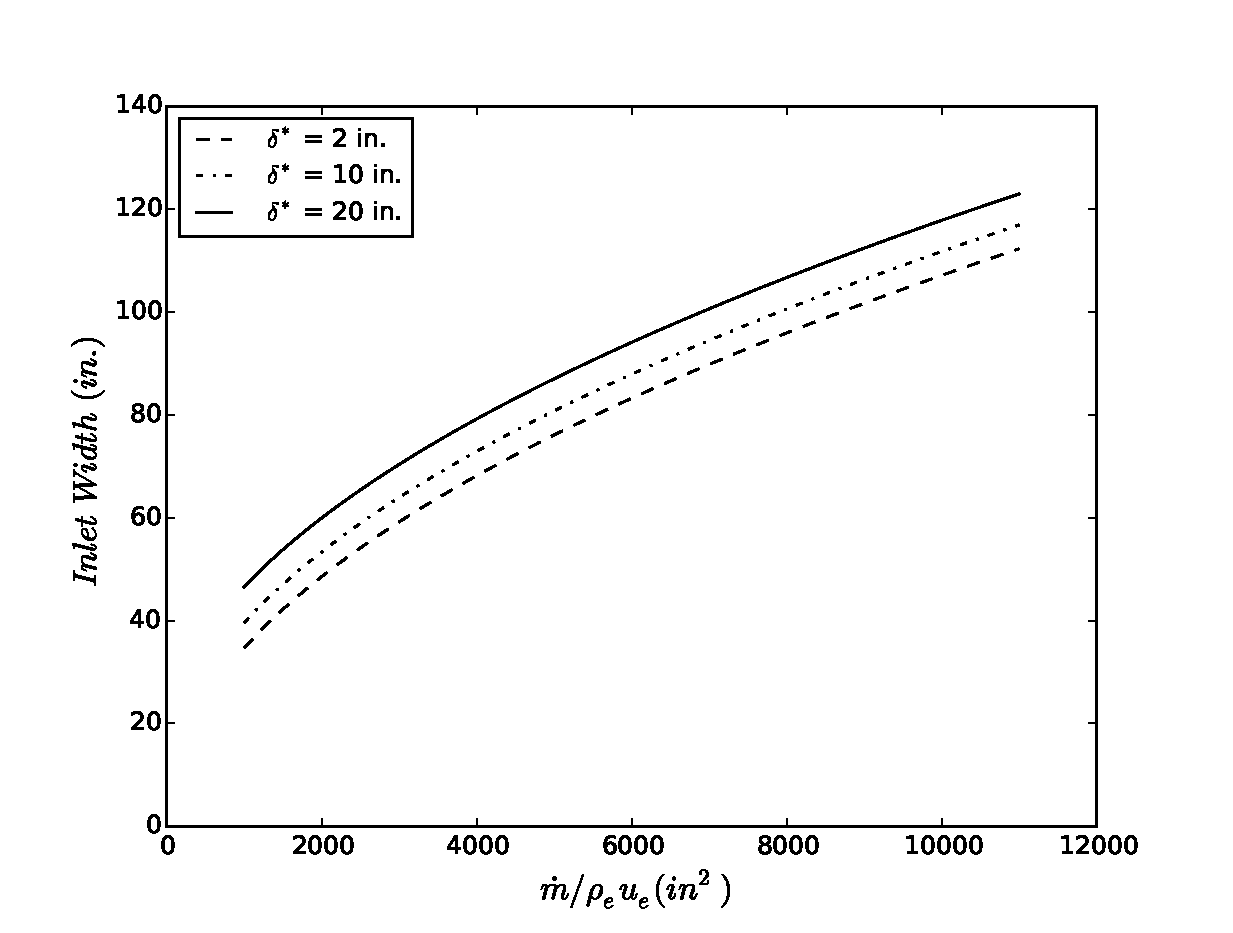
\includegraphics[scale = 0.6, trim = 0mm 0mm 0mm 0mm]{Mass_Flow_Sizing_Influence.eps}
						\caption{Influence of mass flow on the cross-section width solution.}
						\label{Mass_Flow_Sizing_Influence}
					\end{figure}
					
					In general, anything that affects the engine mass flow demand will affect the ingested stream-tube size.  The first obvious choice is the selection of the engine fan pressure ratio, which will have a very large impact on the bypass-ratio of the engine and the ingested mass flow (INSERT REFERENCE).  Figure XXX shows a notional plot of the ingested mass flow vs. fan pressure ratio for a typical modern hi-bypass ratio turbofan engine.  For architectures without traditional turbofan engines, such as a distributed propulsion system, the fan pressure ratio will still have a large impact on the sizing of the fan and the required ingested mass flow (INSERT FELDER REFERENCE /Others?).  
					
					Secondary cycle variables and technology factors additionally affect the mass flow demand of the engine.  For instance, the maximum temperature that the engine can burn at, typically limited by the turbine materials and cooling requirements, will have a significant impact on the available thrust of the propulsion system.  Other less important factors are things like the component efficiencies of the fan, low and high pressure compressors, and the burn efficiency and pressure drop of the combustor.  Anything that ultimately affects the ideal or actual cycle of the engine will have some impact on the desired mass flow and therefore the width of the ingested stream-tube.
					
					Another design feature which has a significant impact on the ingested stream-tube width is the aspect ratio of the inlet aperture area.  If the inlet's width is much larger than it's height, then the amount of captured boundary layer will be greater than the case where the width is equal to the height (aspect ratio = 1), as shown in fig. \ref{AR_Sizing_Influence}.  The designer can therefore increase the aspect ratio of the inlet shape in order to achieve higher levels of ingested boundary layer.  Higher mass flows make the inlet width even more sensitive to the aspect ratio of the inlet for a fixed boundary layer size, as demonstrated in fig. \ref{AR_Sizing_Influence}.
					
					\begin{figure}[htp]
						\centering
						\begin{minipage}{.45\textwidth}
							\centering
							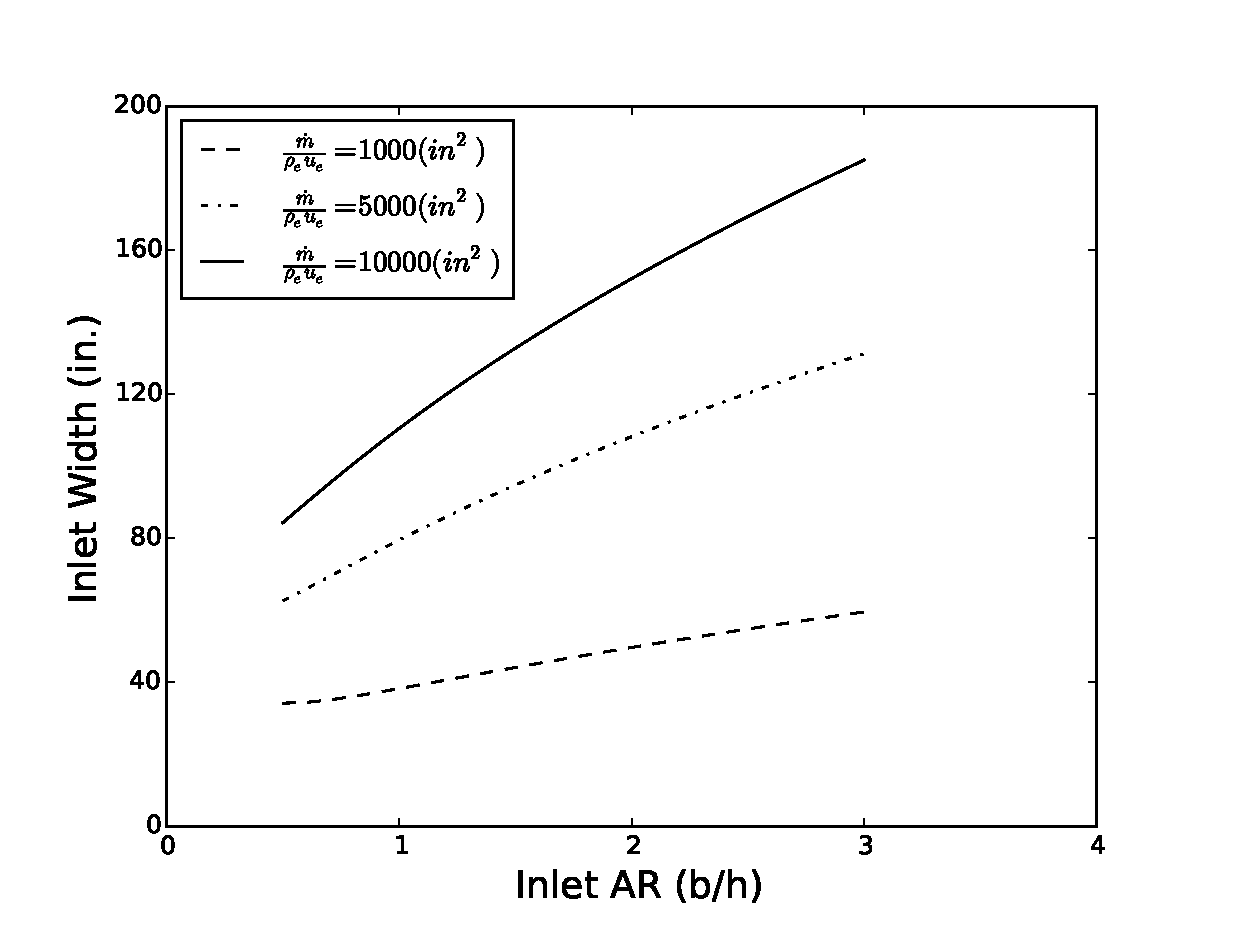
\includegraphics[scale = 0.4]{AR_Sizing_Influence.eps}
							\captionof{figure}{Influence of inlet aspect ratio on inlet width sizing.}
							\label{AR_Sizing_Influence}
						\end{minipage}%
						\hfill
						\begin{minipage}{.45\textwidth}
							\centering
							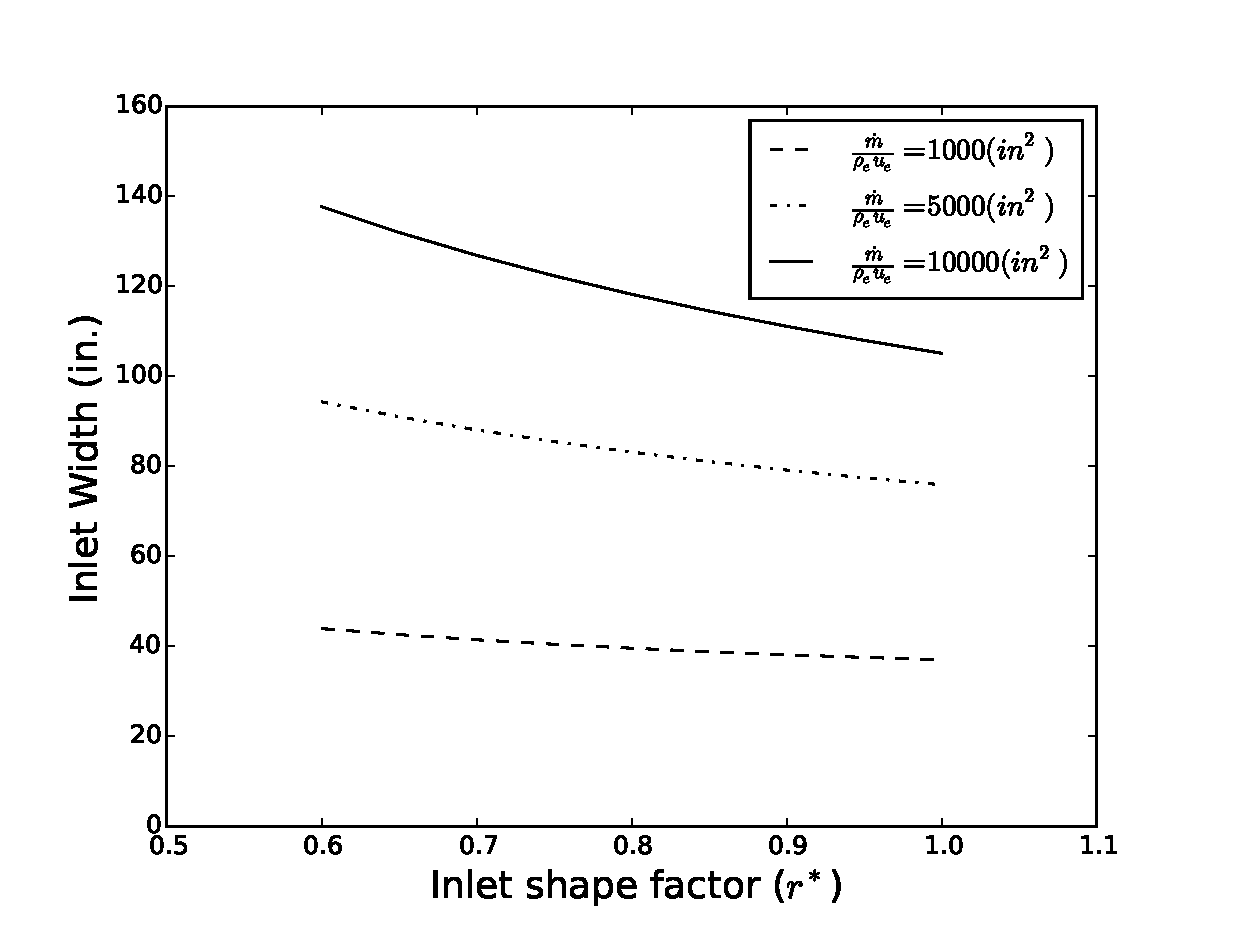
\includegraphics[scale = 0.4]{Rstar_Sizing_Influence.eps}
							\captionof{figure}{Influence of inlet aperture shape on inlet width sizing.}
							\label{Rstar_Sizing_Influence}
						\end{minipage}
					\end{figure}
					The choice of inlet aperture shape also has a relatively weak influence on the inlet width sizing as shown in fig. \ref{Rstar_Sizing_Influence}.  As the inlet is tapered at the top, the width at the bottom of the inlet near the boundary layer must increase to capture more flow.  Table \ref{Inlet_Table} shows several typical BLI inlet shapes for class 2 type BLI with values of $r^*$ and $y(x)$ shown.
					\begin{table}
						\centering
						\renewcommand{\arraystretch}{1.5}% Spread rows out...
						\begin{tabular}	{|>{\centering\arraybackslash}m{4cm}  >{\centering\arraybackslash}m{6.cm} >{\centering\arraybackslash}m{4.cm}|} 					
							\hline
							Shape & y(x) & $r^*$\\ 
							\hline \hline
							\vspace{4mm}
							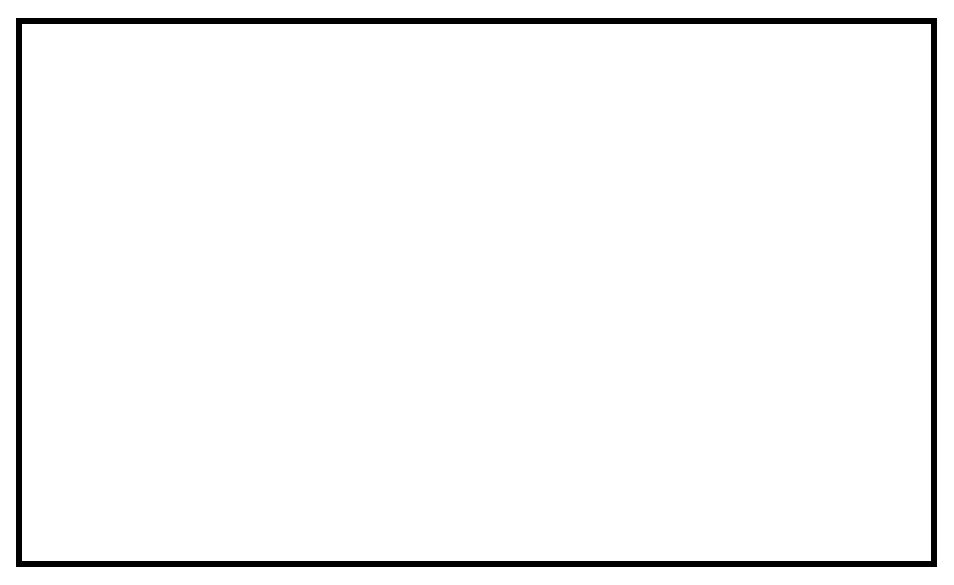
\includegraphics[scale = 0.2]{Rectangular_Inlet.eps}& y(x) = h & $r^* = 1$ \\		
							\vspace{4mm}
							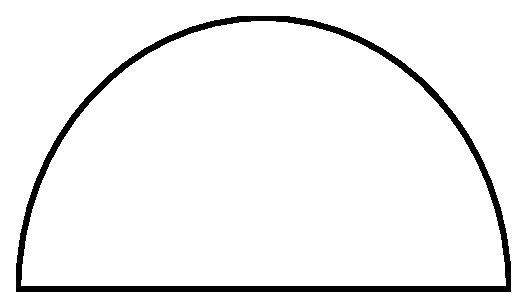
\includegraphics[scale = 0.4]{Semi_Circle_Inlet.eps}& y(x) = $h \cdot \sqrt{1 - 4\frac{\displaystyle(x-b/2)^2}{\displaystyle b^2}}$ & $r^* = \pi/4$ \\		
							\vspace{4mm}
							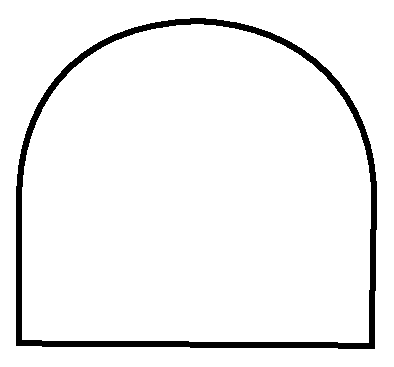
\includegraphics[scale = 0.45]{D_Inlet.eps}& y(x) = $\dfrac{h}{2} + \dfrac{h}{2} \cdot \sqrt{1 - 4\frac{\displaystyle(x-b/2)^2}{\displaystyle b^2}}$  & $r^* = 1/2 + \pi/8$ \\		
							\hline
						\end{tabular}
						\caption{Table showing inlet shapes, y(x), and $r^*$}
						\label{Inlet_Table}
					\end{table}
				
					
					Finally, a fundamental choice with regard to determining the overall system $\beta$ is the location of each propulsor on the upper surface of the airframe.  This involves both the selection of the number of propulsors (something that would effect the engine stream-tube size) and the location of each propulsor both span-wise and chord-wise.  This last choice will affect the size of the boundary layer thickness, as well as the local velocity and static pressure at the inlet.  This has an impact on both the total amount of drag ingested and the overall losses in the inlet and fan due to distortion (REFERENCE).  All of the above discussion leads to the following observation 3:
					
					\vspace{1pt}
					\vspace{5mm}
					\noindent{
						\fbox{
				          \parbox{\textwidth}{
			   					\textbf{Observation 3}:  The engine mass flow size, inlet aperture shape, and location on the vehicle affect the ratio of the ingested drag to uningested drag for class 1 BLI systems.
						  }
						}
					}
				
				\subsubsection{Propulsor Sizing: Class 2 BLI}
				For class 2 BLI systems, the distortion is primarily radial, but the fundamental equation still applies from Eq. \ref{General_Mass_Sizing}, except that the integration is different because of the way that the boundary layer is distributed.  Furthermore, the calculation of the stream-tube width is irrelevant (even meaningless).  Rather, the primary variable is the radius of the propulsor which determines how much mass is ingested. Consider a general flow annulus for a class 2 BLI problem with inner radius $r_i$ and outer radius $r_o$.  The equation for mass flow is then: 
				\begin{equation}
					\dot{m} = \int_0^{2\pi} \int_{r_i}^{r_o} \rho u_x \hspace{1mm} r dr d\theta
					\label{eq:Class2_Sizing_Equation_General}
				\end{equation}
				The definition of \textbf{M} here is slightly different than Eq. \ref{M_Definition}, since it must account for the effect of radius on the area averaging of the velocity:
				\begin{equation}
					\textbf{$M_r(\theta)$} = \int_{r_i}^{r_o} \Big(\rho_e u_e - \rho u\Big) r dr
					\label{eq:M_Definition_Radial}
				\end{equation}														
				From Eq. \ref{eq:M_Definition_Radial}, the final equation for the mass flow of a class 2 BLI propulsor is:
				\begin{equation}
					\begin{aligned}
						\dot{m} = \int_0^{2\pi}\Big[\frac{r_o^2-r_i^2}{2}\rho_e u_e - M_r(\theta)\Big]					
								= \rho_e u_e A  - \int_0^{2\pi}M_r(\theta) \hspace{1mm} d\theta
					\end{aligned}
					\label{eq:Class2_Sizing_Equation_Final}
				\end{equation}
				With the second part of Eq. \ref{eq:Class2_Sizing_Equation_Final} recognizing $A = \pi (r_o^2-r_i^2)$.  If the propulsor is sized with a radius greater than the boundary layer thickness, then the above can be simplified to solve for the required outer radius for a given desired mass flow. The net result is that the propulsor has to be a little bit bigger for a specified mass flow, however if the amount of BLI ingested is large, then the propulsive efficiency improves and the specific thrust increases requiring less mass flow.  
				
				The analysis of Smith \cite{Smith1993} showed that a wake ingesting propeller with class 2 BLI will have significantly improved propulsive efficiency if the wake comprises a large portion of the total vehicle required drag.  In general, for better propulsive efficiency, larger mass flow designs are desirable, since they require less jet velocity to produce the same thrust. However, Smith notes:
				\begin{quotation}
					...when a large part of the craft's wake is ingested by the
					propulsor, there is much less incentive to keep the propulsor
					large. The message here is that, for best efficiency the propulsor
					should be positioned and sized to ingest as much wake
					fluid as possible (increase D/T), but after that, making it still
					larger does not pay off in propulsive efficiency and would
					have other adverse effects such as increased weight.
				\end{quotation}
				For the case of class 2 BLI, this amounts to sizing the propulsor with a large enough radius to consume the entire wake, while for class 1 BLI, there is a more significant design trade-off since larger mass flows imply larger levels of BLI.  
				
				
				\subsubsection{\textbf{Distortion Effects on the Engine}}
					We now turn to the question of how the losses induced by the boundary layer ingestion are developed and also the question of model fidelity requirement with respect to these losses.  Generally, the primary determining factor for the losses of the engine will come from the loss of total pressure due to the presence of the distortion.  This pressure drop can be approximated by integrating the boundary layer velocity profile over the fan face area.  Appendix A describes a mathematical development of the inlet model to be used later in this thesis but also contains an integral formulation showing that the total pressure loss can be approximated by using the kinetic energy defect property defined in Eq. \ref{KE_thickness}, assuming that the density thickness is negligible and a uniform static pressure.  
					\begin{equation}
						\bar{P_t} = P_s + \frac{1}{2}\rho_e u_e^2 \frac{\Big(A-\delta^*-\theta^*\Big)}{\Big(A-\delta^*\Big)} \label{Pt_Integral}
					\end{equation}
					Equation \ref{Pt_Integral} shows that the total pressure loss is proportional to the size of both the boundary layer blockage represented by $\delta^* / A$ and the kinetic energy thickness to area ratio $\theta^* / A$.  This means that a bigger ratio of boundary layer to "clean" flow yields a worse total pressure recovery.  Note that this is in direct contradiction to the analysis developed previously for the BLI benefit, which dictates that ingesting a larger percentage of the boundary layer into the inlet is more beneficial.  The fraction of boundary layer to total flow area is a function of the amount of boundary layer ingested, the value of the 2-D "height averaged" boundary layer thickness and shape, and also the edge velocity of the boundary layer itself -- implying faster flows will tend to produce more losses in a shear layer.  This observation is also corroborated in several experimental sets of data including that of INSERT NASA REFERENCE (BERRIER) and (SHEDON).  These results show that bigger percentages of boundary layer to total flow area yield worse inlet recoveries implying an essential trade-off involved in designing the amount of BLI to be ingested into a system and the subsequent engine size required.  Observation 4 comes the preceeding analysis:
					
					\vspace{1pt}
					\vspace{5mm}
					\noindent{
						\fbox{
					       \parbox{\textwidth}{
										\textbf{Observation 4}:  The boundary layer thickness does not scale directly with the propulsor mass flow, but the stream tube does change. Therefore boundary layer related losses will be different for changes in engine stream tube size, since the total inlet recovery is a function of the ratio of the boundary layer flow to the total flow.									
					       }
						}
					}
	
			\subsubsection{\textbf{Off-Design Analysis}}
				The off-design analysis of BLI engines is something that has not been very extensively researched in the system study literature.  Typically, the focus is on the cruise point efficiency and therefore variations in flight Mach and altitude are not considered especially important for the sizing of the vehicle.  However, the aerodynamic design point of an engine is not the only point of concern.  In fact, the BLIPSS methodology is specifically designed to account for the fact that performance at off-design conditions for highly integrated systems is important to capture.  Therefore, understanding the fidelity requirements for a BLI engine model in off-design is nearly as important as quantifying it for the cruise condition.
	
			\subsubsection{$\mu$ Variation}
				Shedon \cite{Shedon1999} defines a simple model for an inlet, in which the inlet duct loss varies with the cube of the inverse of the mass flow ratio defined as follows:
				\begin{equation}
					\mu = \frac{A_c}{A_\infty} = \frac{\rho_\infty u_\infty}{\rho_c u_c}
				\end{equation}
				The parameter $\mu$ is effectively a measure of how the stream-tube expands or contracts as it approaches the inlet hi-lite area.  The $\mu^3$ variation \cite{Shedon1999} is defined, in its simplest form, as follows:
				\begin{equation}
					\frac{\Delta P}{q_c} = I C_{Fd} + JC_{Fa}\cdot \mu^3 
					\label{mu3_variation}
				\end{equation}
				Here there are two skin friction coefficients, one for the duct and the other for the region of the vehicle prior to entry (as often seen in military aircraft).  The pre-entry flow is the region sensitive to the mass flow ratio variation and is of particular importance for boundary layer ingesting systems.  Usually \ref{mu3_variation} is re-arranged in terms of the free-stream dynamic head rather than the local capture head as follows:
				\begin{equation}
					\frac{\Delta P}{q_\infty} = \frac{I C_{Fd}}{\mu^2} + JC_{Fa}\cdot \mu 
					\label{mu_variation_rearranged}
				\end{equation} 

				An analysis of \ref{mu_variation_rearranged} shows that there are essentially two regimes over which a BLI intake can operate:  one in which the flow accelerates prior to entry ($\mu << 1$), and one where the flow is retarded prior to entry ($\mu >> 1$).  At extremes of these two regimes, the actual intake recovery varies from \ref{mu_variation_rearranged} because of pre-entry separation and lip flow separation, neither of which are included in the derivation of \ref{mu_variation_rearranged}.  Pre-entry separation occurs in regions of extreme flow retardation ($\frac{dP}{dx} > 0$, $\mu >> 1$).  This generally happens in very low mass flow demand regions at high-speeds, such as possibly end of cruise or descent.  Lip separation occurs in the opposite extreme in the low $\mu$ regime where mass flow is very high and velocity is low, which would be of greater concern at the take-off maximum power condition.   
				
				The preceeding analysis again shows that, fundamentally, the determination of inlet losses is a function of how the inlet stream-tube varies as it approaches the inlet. 
	
			\subsubsection{Flight Condition Variation}
				There has been some experimental data defining variations in inlet recoveries at different flight Mach, Reynold's, and mass flow ratio INSERT REFERENCE HERE for inlets designed specifically for BLI applications on large transports.  This data showed that flight Mach number has a very strong influence on the overall recovery, with the mass flow into the inlet playing a significant secondary role which is in congruence with the $\mu^3$ analysis.  The theoretical development by \cite{Shedon1999} also stressed the importance of the skin friction coefficient which significantly increases with the Mach number of the flow.  Furthermore, the \ref{mu_variation_rearranged} gives an expression for duct loss which is normalized by the free-stream head which increases significantly at higher Mach.  The expectation, then, is that the size of the boundary layer relative to the size of a fixed capture height inlet will decrease as the free-stream Mach number is decreased along with both benefit and loss.  This implies that the thrust saving coefficient at low altitude and speeds, especially at the take-off condition, should be relatively lower -- for similar vehicle angles of attack -- than that at high speeds, but that distortion concerns would not be as great.  

			\subsubsection{Angle of Attack Variation}
				In general, subsonic pitot inlet based engines are not generally thought to have much variation in thrust or performance with the angle of attack of the vehicle.  In cases where large angle of attack is required, the inlets can typically be scarfed to provide a favorable flow angle into the intake, thereby reducing any distortion and mitigating loss of pressure recovery.  
				\begin{figure}[htp]
					\centering
					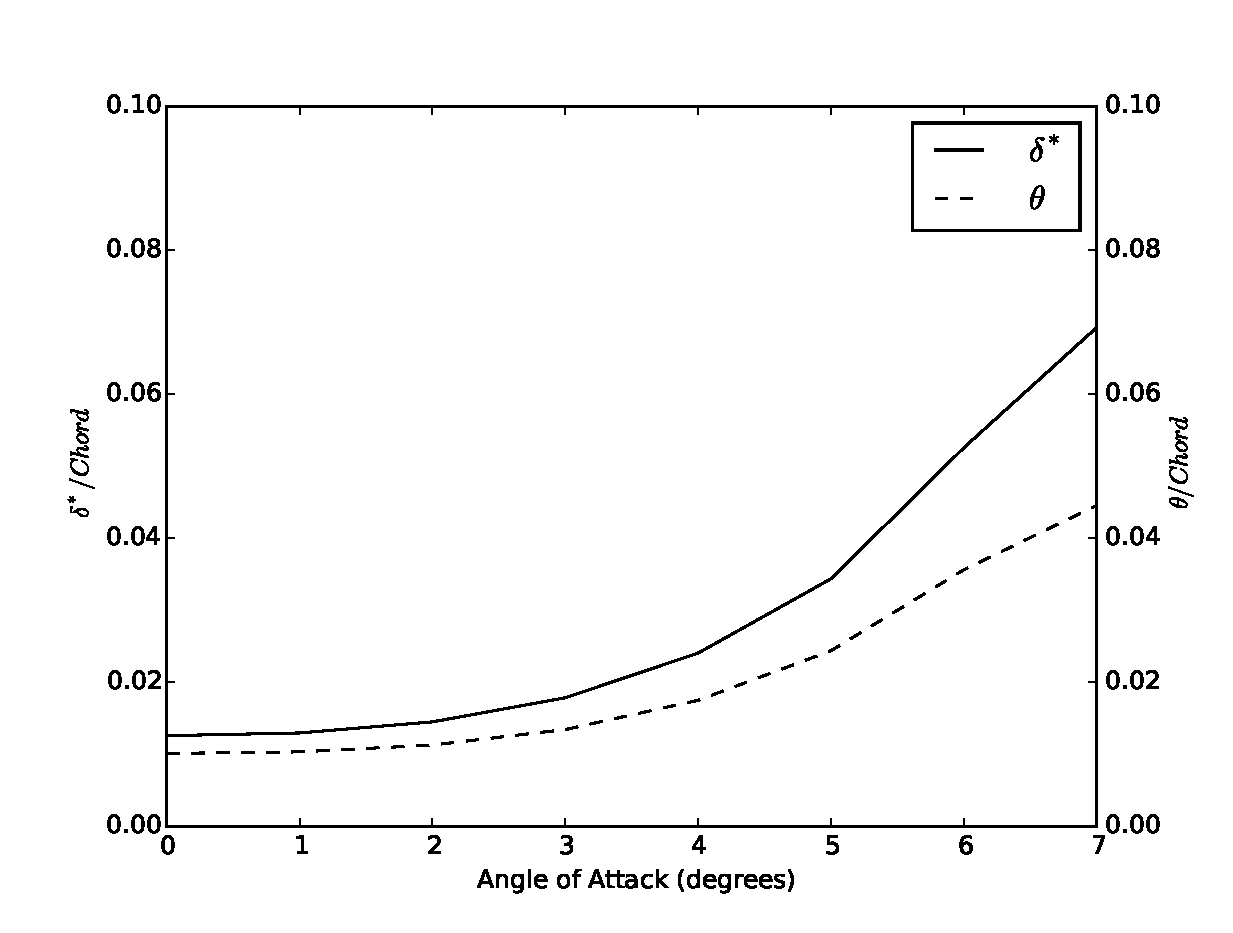
\includegraphics[scale = .5]{plot3-1.eps}
					\caption{Plot showing trend of boundary layer thicknesses vs. airfoil angle of attack for a NACA 2012 airfoil at Mach = 0.7, Re = $10^6$ as predicted by XFOIL}
					\label{plot3-1}
				\end{figure}
				In the case of BLI, this is not possible, and we would therefore expect to see significant variation in the performance of the engine as a function of the vehicle angle of attack.  Figure \ref{plot3-1} shows the variation of boundary layer properties for a NACA 2012 symmetric airfoil at a flight Mach of 0.7 with a Reynolds of $10^5$, as predicted by XFOIL INSERT REFERENCE HERE.
				
				Clearly the boundary layer thickness increases significantly, which will impact the thrust saving coefficient and inlet recovery.  Typical top-of-climb angle of attacks for a hybrid wing body vehicle, such as the N2B or N2A, can be as high as 3.5-5 degrees INSERT REFERENCE HERE, and declines as fuel is burned during cruise and lift required is reduced.  Therefore the variation in thrust, efficiency, and operability as a function of angle of attack, if found to be significant, would be necessary to include in a model at this level.  
	
			\subsubsection{Hypothesis 1}
				Though the discussion above is barely touching the surface in terms of the complexity of an actual boundary layer ingesting flow field, there are some clear basic trends which have arisen from the analysis.  First, the benefit of the system is ultimately a balance between drag recovery and distortion losses, which tend to both increase with the ratio of distorted boundary layer flow to clean flow.  Second is that, at a given design point, any design choice which impacts the size of the ingested stream-tube will impact the amount of boundary layer that is ingested, though those choices will not have an impact on the vehicle boundary layer.  Third, that the boundary layer thickness varies significantly with flight Mach number and angle of attack for a given vehicle.  Fourth, that the losses in the inlet duct leading to the propulsor face will vary significantly with the free-stream mass ratio and the flight condition.  Given that the BLIPSS methodology is intended to be able to account for multiple design conditions, it is therefore necessary, if it is to be used, to account for these fundamental variations in benefits and losses.  Otherwise, changes in flight conditions and power settings will not appropriately match the actual variation in design point performance even at a first level approximation.  From these observations, the following hypothesis is formed:
				
				
				\noindent\makebox[\linewidth]{\rule{\textwidth}{3pt}}				
					 \textbf{Hypothesis 1}:  If multi-design point BLI propulsion system cycle models do not include the physical relationship between the vehicle boundary layer profile, the ingested stream-tube size and its variation, and system power balance and engine losses at critical sizing conditions, then a significant portion of the predicted propulsion system design space will be infeasible.\\
				\noindent\makebox[\linewidth]{\rule{\textwidth}{3pt}}	

	
			\subsubsection{Stall Margin and Stall Constraint}
				\indent Hypothesis 1 deals with the basic modeling requirements for any BLI system.  It is formulated out of a need to appropriately size the system -- based on requirements at multiple flight conditions -- and thereby appropriately form a design space from which early design choices can be made.  The hypothesis is developed in order to properly establish the trade-off between the propulsive efficiency benefit of ingesting more low momentum flow and the losses incurred by doing the same.  The other major component of any boundary layer ingesting system, not addressed by Hypothesis 1, is the impact on the operability of the propulsion system incurred by the ingestion of distorted inflow.  Clearly this is an important component of the problem, and yet it is not typically addressed at the level of conceptual design.  			
				
				Operability is considered to be a constraint on a propulsion system, meaning that adding more is not necessarily desirable beyond that which is required.  The major tool for meeting this constraint is the stall margin stack-up INSERT REFERENCE HERE.  A fan stall margin stack-up typically comprises some percentage which is dedicated to account for possible distortion exiting the inlet at the fan face.  If ingesting boundary layer produces levels or types of distortion which are fundamentally worse than that of typical fan designs, then something must be done in the design to restore normal levels of safe operability.  While it is difficult to determine the efficacy of various distortion mitigating actions in the conceptual design phase, it is worth investigating how conceptual design choices -- the kinds of which the BLIPSS methodology is intended to facilitate -- affect the likely level of stall margin loss due to distortion and therefore the likelihood of being able to restore it to normal levels.  Research question 2 is formulated accordingly:
				\vspace{1pt}
				\vspace{5mm}
				\noindent{
					\fbox{
						\parbox{\textwidth}{
							\textbf{Research Question 2}: How does the stall margin constraint affect the BLI propulsion system design space?			
						}
					}
				}
	
			\subsubsection{\textbf{Distortion Stall Margin Loss}}
				The stall margin stack-up percentage which is included to account for distortion is usually estimated in design based on prior requirements for existing designs.  Testing of fans and compressors then occurs after detail design of the fan is carried out and a test rig can be constructed.  The ARP 1420 INSERT REFERENCE HERE guidelines have developed over the years to guide this experimental process to fruition by giving the operability analyst a standard set of tools and experimental setup to appropriately estimate and measure stall margin loss for specific designs. 
				\begin{figure}[htp]
					\centering
					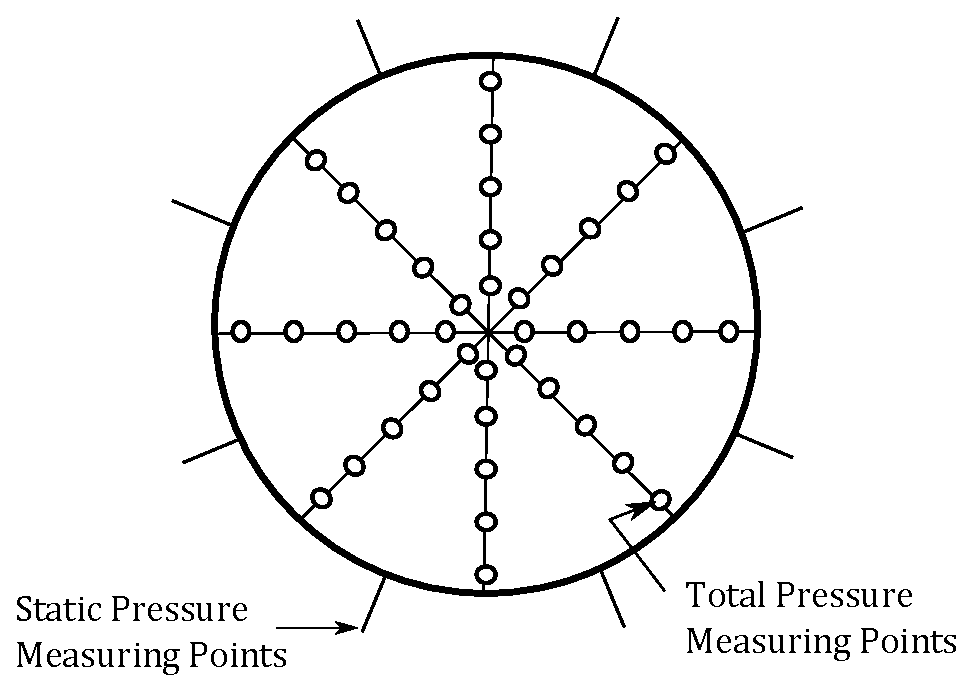
\includegraphics[scale = .5]{Total_Pressure_Rings.eps}
					\caption{Standard ARP 1420 test rig showing static and total pressure probe locations}
					\label{Total_Pressure_Rings}
				\end{figure}
				 The standard rig setup dictated by ARP 1420 is shown in figure \ref{Total_Pressure_Rings} and consists of a set of pressure probes and rings at which the total pressure of the flow is measured.  Typical distortion types can be described in terms of per-rev, which gives measurement of how many low pressure circumferential sections is the blade passing through.  For BLI systems which ingest boundary layer from the upper surface of a vehicle, such as that for the typical HWB type configurations, the distortion usually takes on a 1-per-rev circumferential distortion type.  This type is illustrated for in figure \ref{One_Per_Rev_Diagram}.  The extent is defined as in Eq. \ref{Theta_Extent_Equation} and is representative of the circumferential extent over which the total pressure is lower than the average.  
				\begin{equation}
					\theta^{-}_i = \theta_{2i} - \theta_{1i}
					\label{Theta_Extent_Equation}
				\end{equation}
				The circumferential intensity is defined as:		
				\begin{equation}
					(\frac{\Delta PC}{P}_i) = \frac{(P_{av})_i - (P_{avlow})_i}{(Pav)_i}
					\label{Circumferential_Intensity_Equation}
				\end{equation}				
				\begin{equation}
					(P_{AV})_i = \frac{1}
					{360} \int_0^{360}{P(\theta)_i d\theta}
					\label{Paverage}
				\end{equation}%			
				\begin{equation}(P_{AVLOW})_i = \frac{1}
					{\theta_i^-}\int_{\theta_{1i}}^{\theta_{2i}}{P(\theta)_i d\theta}
					\label{PaverageLow}
				\end{equation}%				
				\begin{figure}[htp]
					\centering
					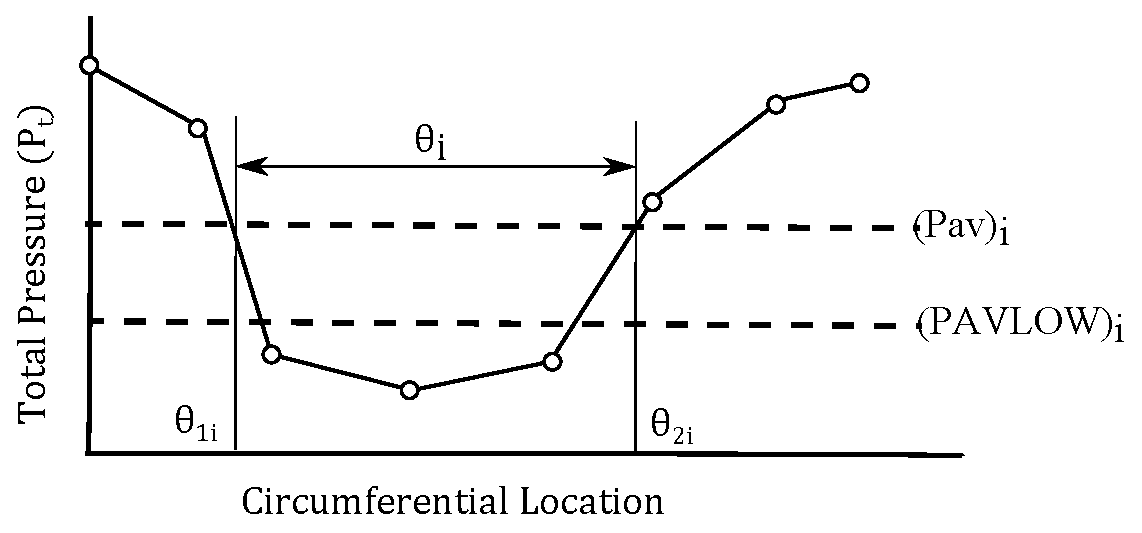
\includegraphics[scale = .6]{one-per-rev.eps}
					\caption{Illustration of a one-per-rev distortion type for a single probe ring.}
					\label{One_Per_Rev_Diagram}
				\end{figure}	
				Then, the total circumferential intensity is the sum of each of the rings.  
				\begin{equation}
					DPCP_{avg} = \frac{1}{N} \sum\limits_{i=1}^{N}(\frac{\Delta PC}{P}_i)
					\label{DPCP_avg}
				\end{equation}%	
				The stall margin loss is typically defined in terms of $\Delta$PRS defined, which is the difference between the clean and distorted stall pressure ratio at constant flow in percentage of the clean stall pressure ratio which is illustrated also in figure \ref{Delta_PRS_Diagram}.
				\begin{equation}
					\Delta PRS = \frac{PRS_{Clean}-PRS_{Distorted}}{PRS_{Clean}}
					\label{Delta_PRS_Equation}
				\end{equation}				
				\begin{figure}[htp]
					\centering
					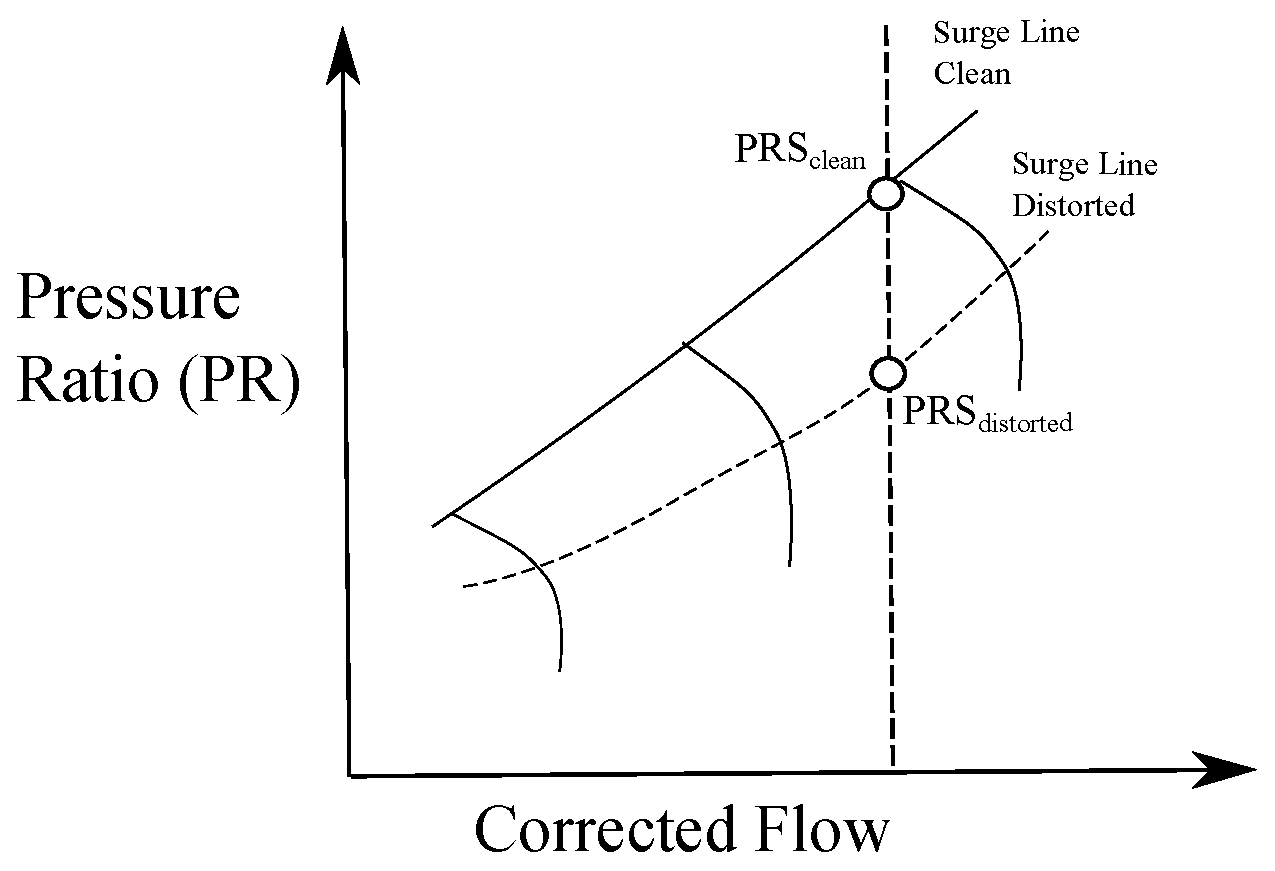
\includegraphics[scale = .45]{Delta_PRS_Diagram.eps}
					\caption{Illustration of the definition of delta PRS with distortion}
					\label{Delta_PRS_Diagram}
				\end{figure}	
				
				Typically the $\Delta$PRS is quantified by correlating it with the intensity defined in Eq. \ref{Circumferential_Intensity_Equation}. An example for classical one-per-rev distortion type would be described in \ref{Classical_Delta_PRS} and is represented with a simple linear correlation.
				\begin{equation}
					\Delta PRS = K_c \cdot DPCP_{avg}
					\label{Classical_Delta_PRS}
				\end{equation}	
				The other type of distortion common to BLI systems is radial pressure distortion, which represents a gradient of the total pressure in the radial direction as is common within a viscous boundary layer.  Radial pressure gradients can significantly affect the compressor characteristic and the pressure ratio at which stall occrus.  The ARP 1420 radial descriptor is defined by Eqs. \ref{Radial_Descriptor} and \ref{PFAV}.
				\begin{equation}
					\Big(\frac{\Delta PR}
					{P}\Big)_i = \frac{PFAV-(P_{AV})_i}
					{PFAV}
					\label{Radial_Descriptor}
				\end{equation}%
				Where,	
				\begin{equation}
					PFAV = \frac{1}
					{N} \sum\limits_{i=1}^{N} (P_{AV})_i
					\label{PFAV}
				\end{equation}%
				The standard DC($\theta$) which represents a descriptor for complex distortion types containing both circumferential and radial is then defined as follows:
				\begin{equation}
					DC(\theta_E) = \frac{1}{N} \sum\limits_{i=1}^{N}\Big[\Big(1-\frac{\Delta PR}{P}\Big)_i \cdot 
								   \Big(\frac{\theta_i}{\theta_E}\Big) \cdot 
								   (\frac{\Delta PC}{P}_i)\Big] \cdot PFAV/q_{avg}
					\label{DC_Theta}
				\end{equation}%
				This descriptor, which combines the types of distortion which can be represent various complex patterns can also be correlated with $\Delta$PRS, which is standard practice for experimental testing and quantification of distortion stall margin loss INSERT REFERENCE HERE.  
				
			\subsubsection{Canonical Example}
				Consider now the case of a circular fan aerodynamic interface plane defined in terms of polar coordinates (r, $\theta$) and with a standard ARP 1420 set of rakes applied to it. The hub-to-tip ratio of the fan is fixed at 0.45. The centerline ($\theta = 0$) is represented by a $1/7^th$ power law velocity distribution typical of turbulent flat-plate boundary layer profiles with a 99\% thickness defined as $\delta$.  The ratio of the boundary layer thickness to fan blade span is $\delta$/h.
				\begin{equation}
					\frac{u}{u_e} = \Big(\frac{y}{\delta}\Big)^{1/7}
					\label{1/7th_Power_Law}
				\end{equation}%
				The circumferential variation in the velocity distribution is assumed to be defined as follows \cite{RodriguezThesis}:
				\begin{equation}
					p_t(r, \theta) = p_{t_l}(r)cos^{10}(\theta)+p_{t_h}(r)\Big[1-cos^{10}(\theta)\Big]
					\label{2D_Circumferential_Mapping}
				\end{equation}%	
				\begin{figure}[htp]
					\centering
					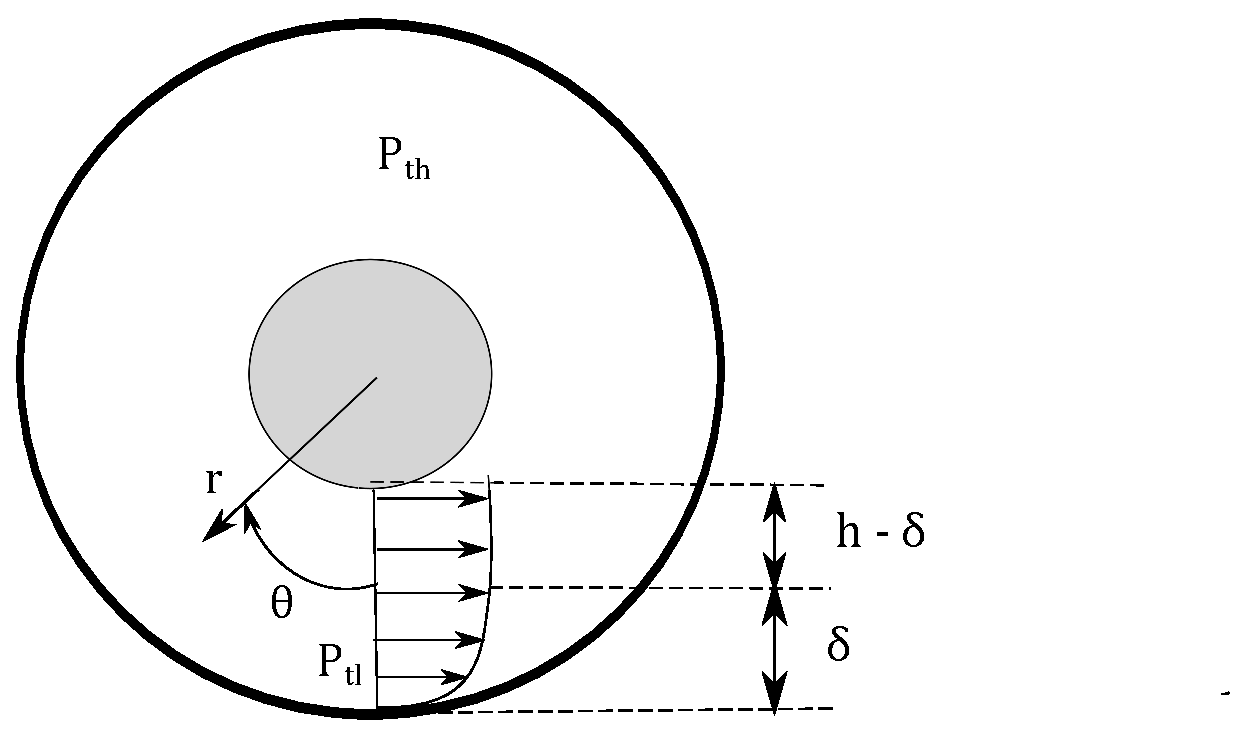
\includegraphics[scale = .5, trim = 0mm 0mm 50mm 0mm]{Fan_AIP_Diagram.eps}
					\caption{Illustration of the Notional Fan Face AIP}
					\label{Delta_PRS_Diagram}
				\end{figure}

				Applying the above parameterizations and assumptions in velocity profile, a 2-D fan face representation can be constructed and the distortion descriptor DC($\theta_E$) can be calculated.  Some values for the pressures and temperatures assumed in this case are shown in table \ref{Distortion_Example_Table}.  Figure \ref{AIP_Rake_Data} shows the AIP pressure distributions for 5 typical rakes generated for a boundary layer thickness to blade height ratio of unity.
				\begin{table}[htp]
					\begin{center}
						\begin{tabular}{p{3cm} | p{3cm} } 
							\hline
							Parameter & Value \\ 
							\hline 
							$P_{th}$ & 15 psia \\ 
							$M_e$ & 0.65 \\ 
							$r_h/r_t$ & 0.45 \\ 
							$r_t$ & 56 in. \\ 			
							\hline
							\hline
						\end{tabular}
						\caption{Distortion Example Parameters}
						\label{Distortion_Example_Table}
					\end{center}
				\end{table}  
				\begin{figure}[htp]
					\centering
					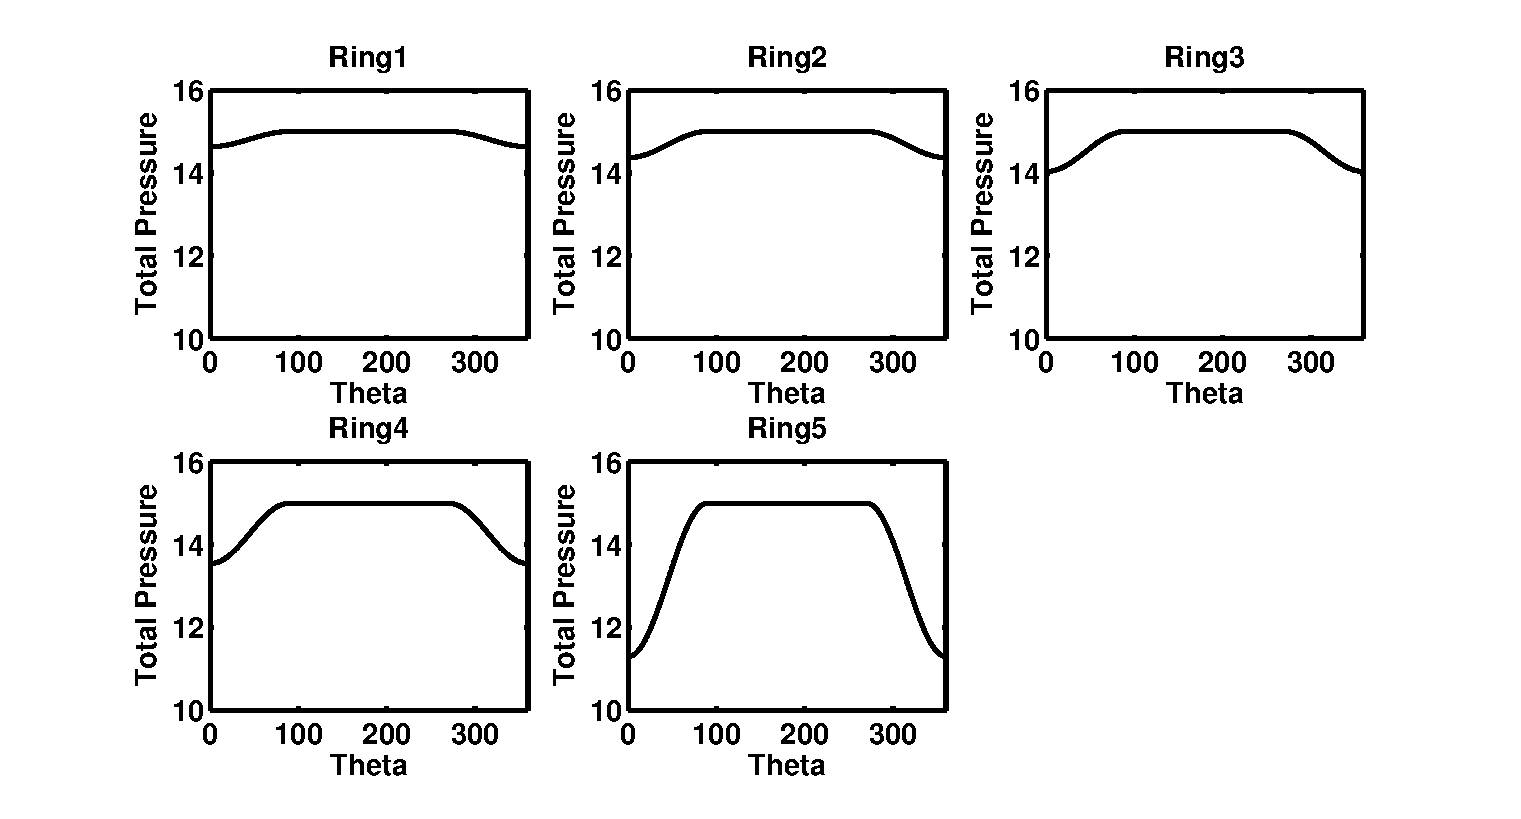
\includegraphics[scale = 0.6]{AIP_Rake_Data.eps}
					\caption{Example fan face ring total pressure distribution.}
					\label{AIP_Rake_Data}
				\end{figure}
				From these distributions, the rake data can be used to calculate the distortion descriptors.  The boundary layer height to blade height ratio was varied from 0.1 to 2 and the distortion descriptors are calculated.  The results -- shown in figure \ref{distortion_example_results} illustrate what happens when the thickness of the boundary is increased relative to the size of the clean flow area.
				\begin{figure}[htp]
					\centering
					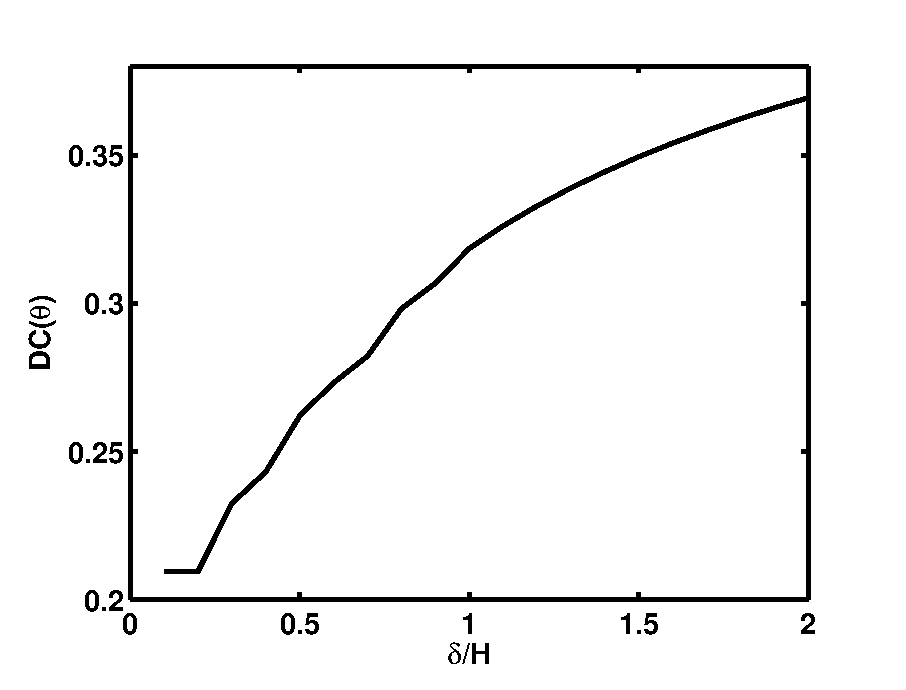
\includegraphics[scale = 0.6]{distortion_example_results.eps}
					\caption{DC($\theta$) descriptor plotted vs. boundary layer thickness ratio.)}
					\label{distortion_example_results}
				\end{figure}
							
			\subsubsection{Hypothesis 2}				
				Since DC($\theta$) generally correlates directly with $\Delta$PRS, it stands to reason that increasing the boundary layer thickness to height ratio will harm the stability margin of the fan substantially.  This could, in theory, place limits on the size of the propulsor in relation to the size of the boundary layer in order to maintain operability.  From observation 2, it has been established that the benefit of BLI is a strong function of the same ratio, implying that operability may limit the cycle designer's ability to ingest more drag within imposing an operability problem on the system.  If the cycle designer is given a hard target on what the allowable stall margin loss ($\Delta$PRS) is at the conceptual phase, then this would limit the possible benefit that a BLI propulsion system would give.  Hypothesis 2 is therefore derived from this simplified analysis and is stated as follows:
							
				\noindent\makebox[\linewidth]{\rule{\textwidth}{2pt}}									
					\textbf{Hypothesis 2}: The operability constraint limits the thrust saving coefficient achievable by a given propulsor.\\			 	  			
				\noindent\makebox[\linewidth]{\rule{\textwidth}{2pt}}				
				
				 There a few caveats worth mentioning to clarify the statement of Hypothesis 2.  It does not necessarily say that the constraint will be an active constraint on the system.  For instance, if something else, such as engine core "size-effect" losses or other practical concerns limit the available amount of ingestion, then the constraint would still be present in the design space but would not affect the design choice made. Also note that the hypothesis is made in terms of a single propulsor, not necessarily an entire system.  There may, in fact, be system configurations in which part of the propulsion system ingests boundary layer while another part does not.  In this case, increasing the thrust saving coefficient of the BLI propulsor would not necessarily increase the overall $\beta$ of the system, but it would decrease operability via distortion increase. 
	
			\subsubsection{BLI Modeling Phase Process}
				Hypotheses 1 and 2, if substantiated, imply a solution to research question 1:  namely that the BLI modeling phase should consist of building models which accurately represent the relationship between the major conceptual design variables determining the level of BLI ingested and losses in performance and operability of the system.  The following modeling algorithm for the BLI modeling phase is thus developed from this understanding and the preceeding theoretical analysis: 	
							
				\vspace{5mm}
				\underline{Prior to Analysis}
				
				\begin{enumerate}[label = \protect\circled{\arabic*}]
					\item{Establish vehicle airframe geometry}
					\item{Identify BLI propulsor type:  Class 1 or 2}					
					\item{Establish aerodynamic cross-section stack-up (based on step 1):  Lateral for C1;  rotational for C2}
					
					\underline{For each flight condition and propulsor location:}
					
					\item{Compute BL defect property from ``clean'' airfoil analysis ($\delta^*, \theta, \theta^*$) at $(x,y)_{inl}$, $(x,y)_{TE}$, and $(x,y)_{trefftz}$}								
					\item{Approximate $\nu =K_{\infty_{BLI}}/K_\infty$ based on BLI type.}
					
					\underline{For each cycle analysis iteration}
					\item{Compute BLI thrust term ($\beta \cdot \Phi_p^*$) based on BLI type (Eq. \ref{Beta_Calculation_Specific} for C1, Eq. \ref{eq:Class2_Beta_Equation} for C2)} 	
					\item{Compute $\displaystyle\frac{A_o}{A_c}$  and inlet losses based on inlet BL properties.}
					\item{Estimate inlet distortion and compute propulsor operating line}								
					\item{Estimate $\Delta PRS$ and $\Delta \eta_F$}
				\end{enumerate}
				
		\subsection{Architecture Integration Phase}
			With advances in aerospace concepts toward more fuel efficient, revolutionary aircraft, such as the HWB, there are many possible types of architectures that could potentially become viable.  Varying numbers of BLI engines could be used, such as 2, 3, 4, or 5 engine BLI turbofans INSERT REFERENCE.  The concept of turbo-electric distributed propulsion has also been investigated as a possible architecture, in which there are turbo-generators which do not ingest boundary layer but transfer power, via an electrical distribution system, to a propulsor array which spans the upper surface of the vehicle INSERT REFERENCES HERE.  Each of these architectures can take advantage of boundary layer ingestion, with some of them ingesting more overall stream-tube than others.  Figure \ref{Architecture_Examples} shows several of these possible architectures, with varying propulsor numbers and locations on the upper surface of the HWB.  All of these potential propulsion system architectures need to be evaluated in comparison to each other, but also need to be properly sized at the conceptual level in order to make legitimate comparisons of overall fuel burn and weight between the systems.  
			\begin{figure}[htp]
				\centering
				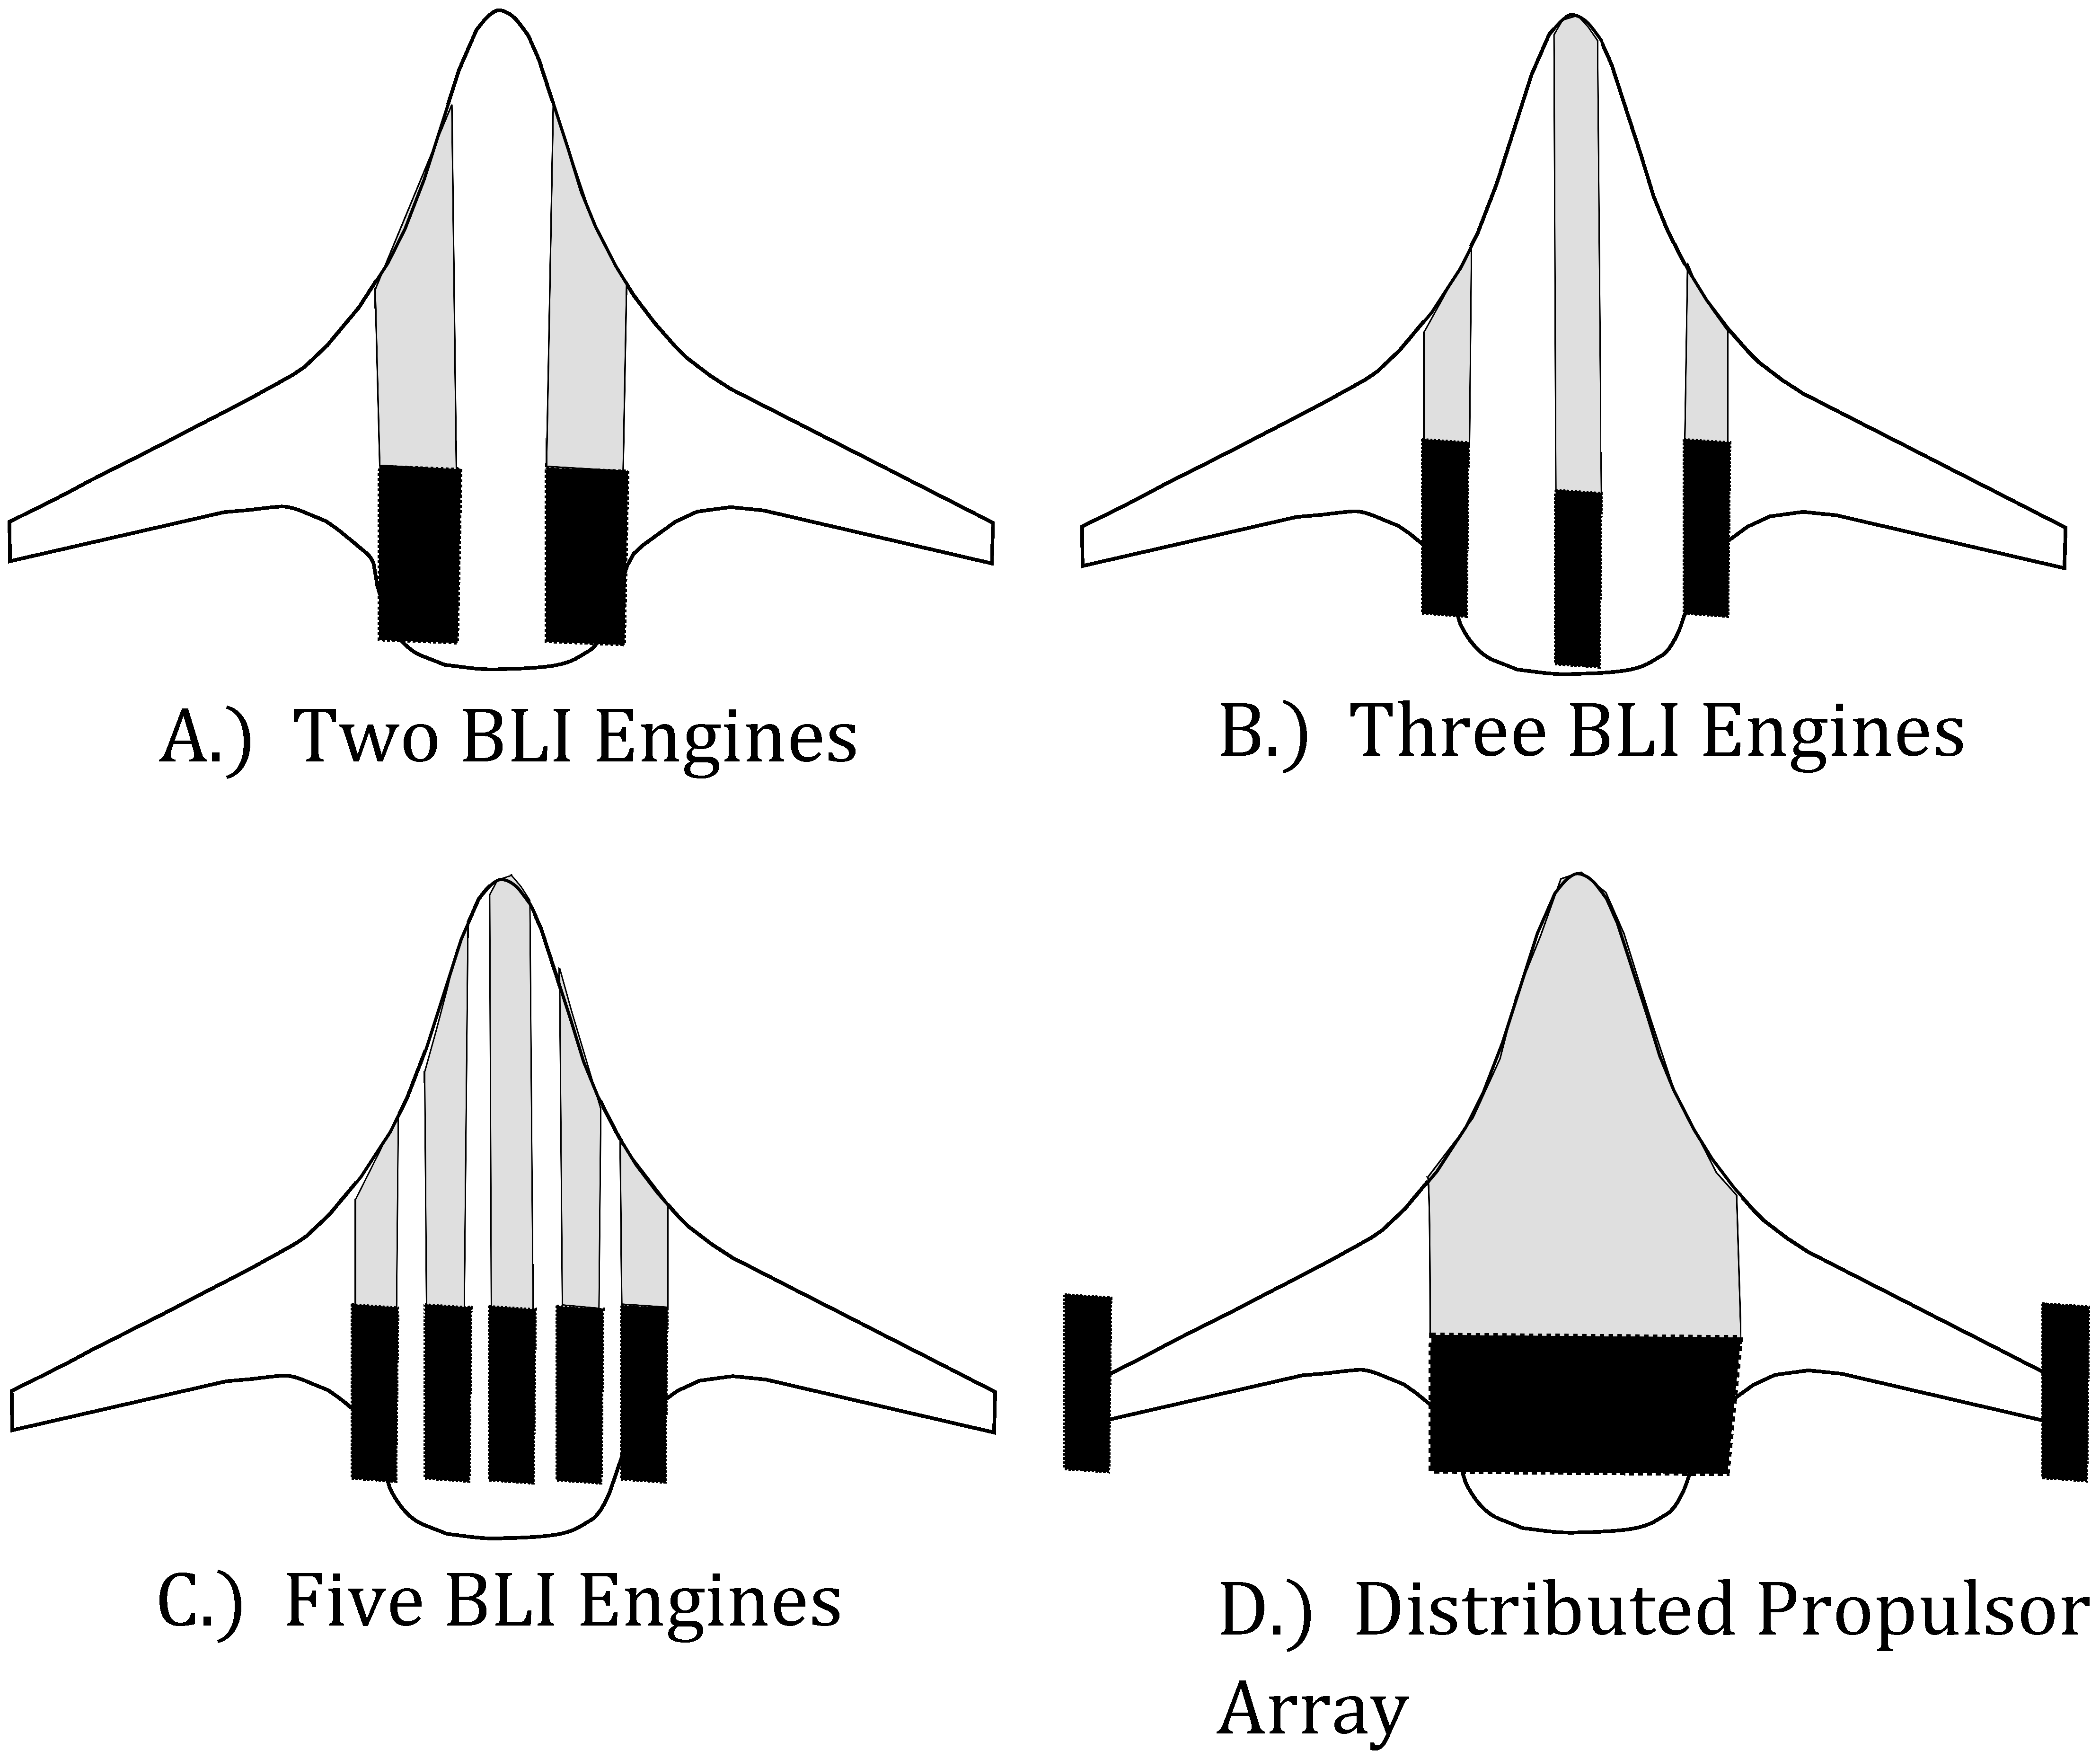
\includegraphics[scale = 0.125]{Architecture_Examples.eps}
				\caption{Examples of potential propulsion system architectures for an HWB aircraft.}
				\label{Architecture_Examples}
			\end{figure}		
		
			\subsubsection{Observations and Research Question 3}
				As noted in chapter 2, the problem of integration for BLI systems in relation to the MDP sizing process is that the airframe can impact each propulsor/gas generator in different ways depending on the location of the propulsor on the airframe.  This relates to both the nature of the boundary layer at the inlet location, which will significantly impact the recovery, and the overall amount of boundary layer ingested and recovered by the engine.  Factors which impact this are mostly related to the airframe geometry, including things such as the airframe airfoil design (thickness-to-chord, camber, etc) and the overall chord length.  For example, in general the boundary layer thickness will increase as a function of the axial location along a surface.  A simple demonstration is seen in Eq. \cite{Flat_Plate_Chord} for a turbulent flat-plate boundary layer -- assuming a 1/7th power law -- which represents the increase of the boundary layer thickness with axial position  INSERT REFERENCE HERE.  
				\begin{equation}
					\frac{\delta}{x} = \frac{0.3747}{(Re_x)^{0.2}}
				\end{equation}
				This means that if chord length of the airfoils tapers, as it clearly does for the HWB, then the boundary layer will decrease as a function of the \%Chord, and the amount of wake recovery generated by ingesting the boundary layer will be less.  This is also saying that the inner portion of the HWB center body, which is much longer and therefore thicker, will generate more viscous profile drag.  Thus, choices of where the propulsors are placed will have an impact on the overall thrust saving coefficient, inlet recovery, and the stall margin loss of the system.  To further corroborate the idea that this will significantly impact the system, one need only look read reference INSERT N2B reference here, in which the boundary layers of the outboard sections of an HWB design (Boeing N2B) were found to be significantly smaller than the outboard (factor or 1/2).  Furthermore, the engine aerodynamic interface planes had significantly different levels of distortion and overall recovery between them.  The above considerations illustrate the nature of the integration problem vis a vis the propulsion system cycle analysis, and research question 3 is formulated as a result:
				
			\vspace{1pt}
			\vspace{5mm}
			\noindent{
				\fbox{
					\parbox{\textwidth}{
						\textbf{Research Question 3}: How can multiple design points, different BLI propulsion system architectures, and variations in inlet properties between propulsors/engines at a given flight condition be accounted for in BLI propulsion system conceptual design?						 						  			
					}
				}
			}
			
		\subsubsection{Methodology Development}
			To establish a way of dealing with the above research question, it is first necessary to understand how the MDP methodology operates in practice.  Figure \ref{Sequential_MDP_Diagram} shows the sequential SDP process.  This process is designed for a single engine and design point.  The idea is to iterate between the desired off-design conditions to check that the requirements at those conditions are met.  The operating thrust at the design condition can be altered to then satisfy the off-design conditions.  
			
			\begin{figure}[htp]
				\centering
				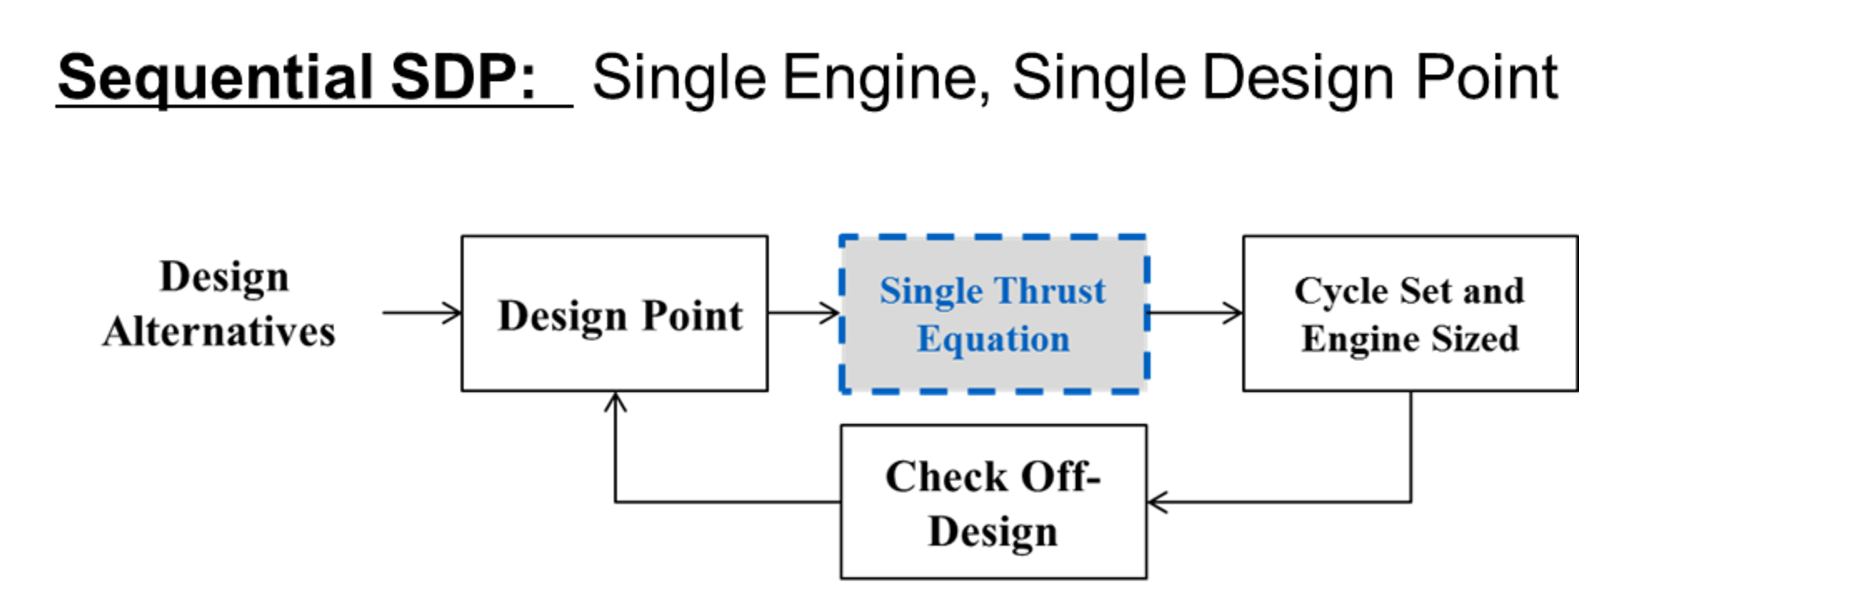
\includegraphics[scale = 0.45]{Sequential_MDP_Diagram.eps}
				\caption{Illustration of Sequential Single Point Design}
				\label{Sequential_MDP_Diagram}
			\end{figure}	 
			
			By comparison, the multi-design point process, illustrated in figure \ref{MDP_DesignPoint_Diagram}, is intended to remove the iteration with the off-design conditions in order to automate the design process to produce a design space with off-design conditions automatically satisfied. 
			
			\begin{figure}[htp]
				\centering
				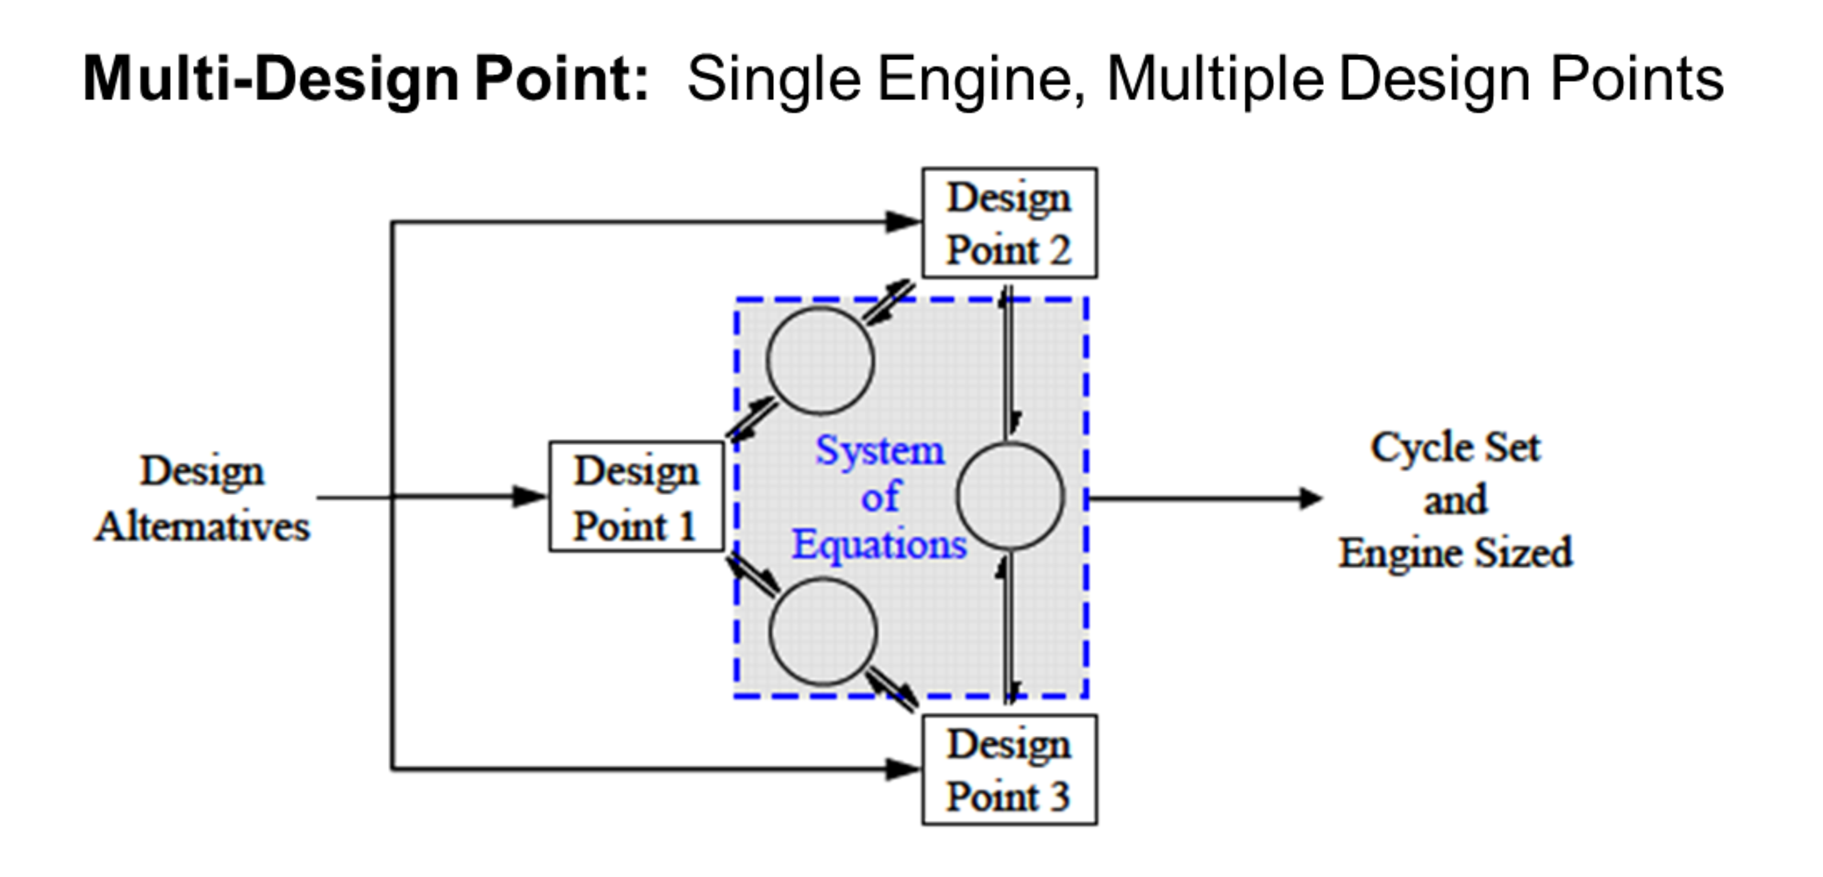
\includegraphics[scale = 0.4]{MDP_DesignPoint_Diagram.eps}
				\caption{Illustration of Multi-Design Point Process}
				\label{MDP_DesignPoint_Diagram}
			\end{figure}	 
			
			To account for the performance of the engine/propulsor at different inlet conditions, the MDP process from \ref{MDP_DesignPoint_Diagram} could be iterated with an off-design condition where the inlet conditions are changed.  Then, the engine could be rematched according to the change in performance that is calculated.  Instead of this manual process, which is analogous to the SDP process, the inlet conditions can be included as "Design Points" in the MDP analysis.  To extend this even further, the possibility of having different sized propulsors can be included in this, which would mean that each unique propulsor/inlet combination at each flight condition would be considered a "Design Point" in the automated MDP process.  This process is illustrated in figure \ref{MEMDP_DesignPoint_Diagram}.  
			
			There are two major changes which occur from this view of the multi-engine/propulsor MDP process:  first there needs to be some set of rules which relate the design and operation of the propulsor at each flight condition; second is that the thrust calculated is now the sum of the separate propulsor thrusts from each "design point" times the number of propulsors included in that design point (since it is possible to have multiple propulsors represented by a single design point).	The rules required for the completion of the ME-MDP process are classified into two categories:  design rules, and power management rules.  These are discussed in more detail in the following section.				
			
			\begin{figure}[htp]				
				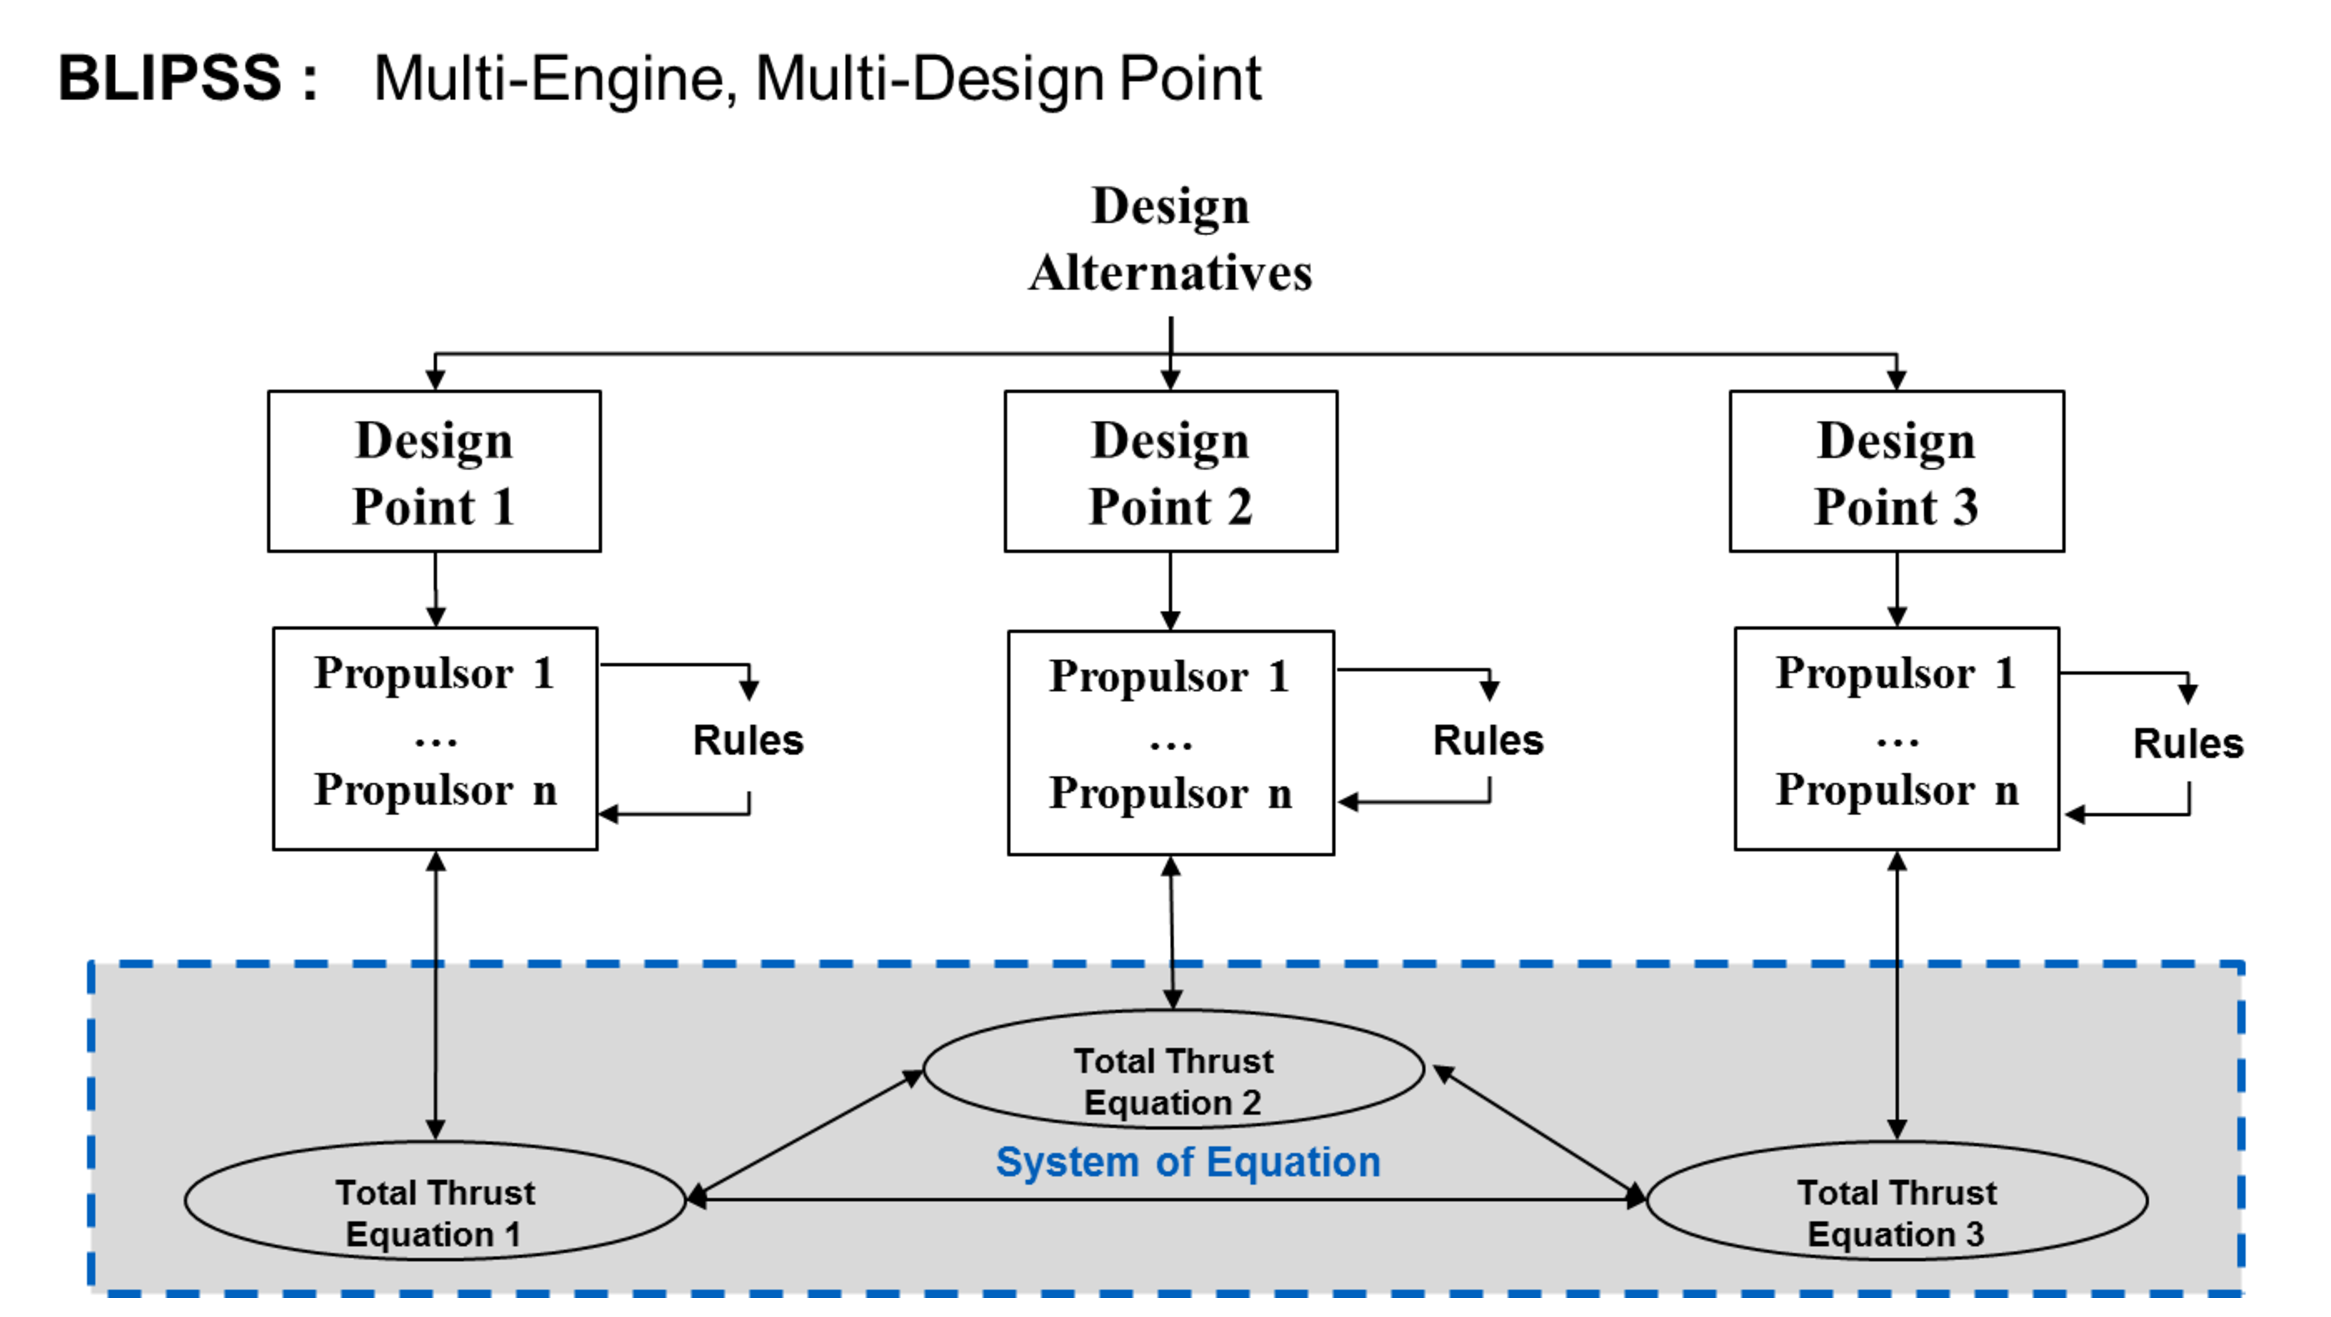
\includegraphics[scale = 0.45, trim = 25mm 0mm 0mm 0mm]{MEMDP_DesignPoint_Diagram.eps}
				\caption{Illustration of Multi-Engine Multi-Design Point Process}
				\label{MEMDP_DesignPoint_Diagram}
			\end{figure}
			
		\subsubsection{Design Rules}			
			Design rules are defined as a mathematical relationship that relates the size of a propulsor or propulsor components at its aerodynamic design point to another uniquely different propulsor at the aerodynamic design original propulsor.  If there is only a single engine/propulsor designed, then there is no need to have additional design rules.  If "k" unique propulsors are designed, then there can be as many as $\sum\limits_{i=1}^{k} N_{comp} - 1$ design rules, where $N_{comp}$ is the number of aerodynamic design points for propulsor "i".  For example, if 2 different turbo-fan engines were sized for a 3-Engine HWB with BLI (a case to be considered in detail later in this document), then the number of design rules is exactly 1.  If there is only a single aerodynamic design point (only 1 propulsor designed), then there is no required design rule.  Examples of design rules for each of the propulsor architecture layouts from figure \ref{Architecture_Examples} are shown in table XXX.  Another interesting aspect of the creation of design rules is that it creates additional cycle design variables for the system, which may have a significant impact on the amount of BLI ingested by each propulsor and potentially the system as a whole.						
		
		\subsubsection{Power Management Rules}
			Power management rules are mathematical relationships that relate the power output of one propulsor \textbf{at each design point} to the power output of another.  In general, the amount of power provided by a propulsor will be proportional to the speed, meaning the power management scheme will pertain to the speeds of the fans/propellers.  Some engine manufacturers use the fan speed $(N_1)$ as the primary power management variable which is measured in the engine, while others use engine pressure ratio (EPR) to correlate thrust INSERT REFERENCE HERE.
			
			Power management rules are specified at each flight condition, except for the aerodynamic design points of the propulsors, since turbo-machinery components are, by definition, at 100\% speed at their ADP.  If one propulsor is at its aerodynamic design point, and another is not, then the power management rule and the design rule are the same thing at that point, since setting the size of the propulsor will also set the relationship between the power output of the propulsors.  Therefore, the number of additional power management rules (on top of the design rules) required can be computed by Eq. \ref{Power_Management_Number},	where k is the number of unique propulsor/inlet combinations, "P" is the number of design points, and $N_{comp}$ is the number of ADPs for each propulsor.
			\begin{equation}
				N_{pm} = \underbrace{P(k-1)}_\text{Design + PM Rules} - \underbrace{\Big(\sum\limits_{i=1}^{k} N_{comp}\Big) - 1}_\text{Design Rules}
				\label{Power_Management_Number}
			\end{equation}		
		
		\subsubsection{Engine Matching Relations}
			The normal engine matching relations are a set of independent variables and dependent relations that are solved by the Newton-Raphson solver in the MDP method.  The independent variables in the engine matching relations are typically the fuel-to-air ratios of the burner, while the dependent relations are equations which set the thrust to a desired level of thrust or the speed of the engine/propulsor to a desired fraction of the design speed (which correlates with thrust).  As such, the MEMDP method must necessarily modify the engine matching relations to accomodate the new architectural arrangement.  
			
			If a propulsion system has k uniquely defined propulsor/inlet condition combinations and the $i^{th}$ combination contains $m_i$ propulsors, then the total number of propulsors is defined by:			
			\begin{equation}
				n = \sum_{i=1}^{k}m_i 
			\end{equation}
			and the total thrust, in the case of BLI is defined by:
			\begin{equation}
				F_{n_{BLI}} = \sum_{i=1}^{k}m_i (F_{n_{BLI}})_i
			\end{equation}
			As such, the thrust saving coefficient and thrust specific fuel consumption are also computed as the sum.
			\begin{equation}
				TSC = 1 - \dfrac{\sum_{i=1}^{k}m_i F_{n_i}}{\sum_{i=1}^{k}m_i \dfrac{F_{ni}}{(1-TSC_i)}}
			\end{equation}
			
			\begin{equation}
				TSFC = \dfrac{W_f}{F_{n_{BLI}}} = \dfrac{\sum_{i=1}^{k}{W_{fi}}}{\sum_{i=1}^{k}{(F_{n_{BLI}})_i}}
			\end{equation}
			
			Finally, the total amount of engine matching relations is precisely equal to $P + N_{pm}$.  These engine matching relations comprise the vector of independent variables which affects the power output of each propulsor and the vector of dependent thrust or power balance relations (power management rules plus P total thrust relations).  If k is greater than unity, and the additional (k-1) unique propulsors are allowed their own design points, then the number of engine matching relations is reduced and each replaced with a single cycle design relation for the uniquely designed propulsor.						
			
		\subsubsection{Alternative Approaches and Hypothesis 3}
			The major alternative approach to dealing with the problem of inlet condition variation is to add an augmentation term to the boundary layer ingestion term in the power balance.  This approach will be called the "augmented power balance approach".  This would work by sizing a single propulsor in a traditional manner, but with the wake recovery term for that single propulsor augmented to reflect the difference in wake-recovery between the different propulsors on the vehicle.  This approach has the difficulty of not always knowing "a-priori" exactly how much wake recovery will be lost or gained due to that variation and it also does not capture differences in inlet recovery between the propulsors induced by the boundary layer disparity.  It also does not allow the new degrees of freedom appropriated by the additional design rules and power management rules in the ME-MDP method.  This alternative approach was used in an example system level study of a distributed propulsion architecture by MIT INSERT REFERENCE HERE.  A comparison of this approach will be shown in later sections.  
			
			With the above description of the proposed ME-MDP approach to be used within the BLIPSS design method, the following hypothesis has been formed in relation to research question 3.  
			

			\noindent\makebox[\linewidth]{\rule{\textwidth}{3pt}}				
			\textbf{Hypothesis 3}: Differing inlet conditions for BLI propulsion systems can be accounted for by using a modified simultaneous MDP approach and specifying the number of engines, inlet conditions, a set of power management rules, design rules, and by modifying the engine engine matching relations to relate to the total vehicle thrust rather than thrust per engine.  If the difference in the local inlet properties are large, this approach will yield increasingly different performance predictions than if the traditional single engine or the augmented power balance approach is used.  		\\										 						  			
			\noindent\makebox[\linewidth]{\rule{\textwidth}{3pt}}				
	
		\subsubsection{Canonical Problem and Research Question 4}
			The test problem for hypotheses 1-3 chosen for this thesis is the N2A boeing HWB design.  The selected propulsion architecture to test hypothesis 3 is a 3-engine turbo-fan based architectures.  As such, this section will define the architecture integration phase and pose a relevant research question for this canonical problem with regard to the power management and design rules.  A diagram of the 3-engine configuration is shown below in figure \ref{N2A_3_Engine} with some key parameters for the system defined.  The propulsion system will, in order to maintain symmetry, always have one "inboard" engine at the aircraft centerline (thicker boundary layer) and an outboard engine which is at some parametric location value.  This value will be used to test hypothesis 3 and to determine engineering trades on the system overall.		
			
			\begin{figure}[htp]		
				\centering		
				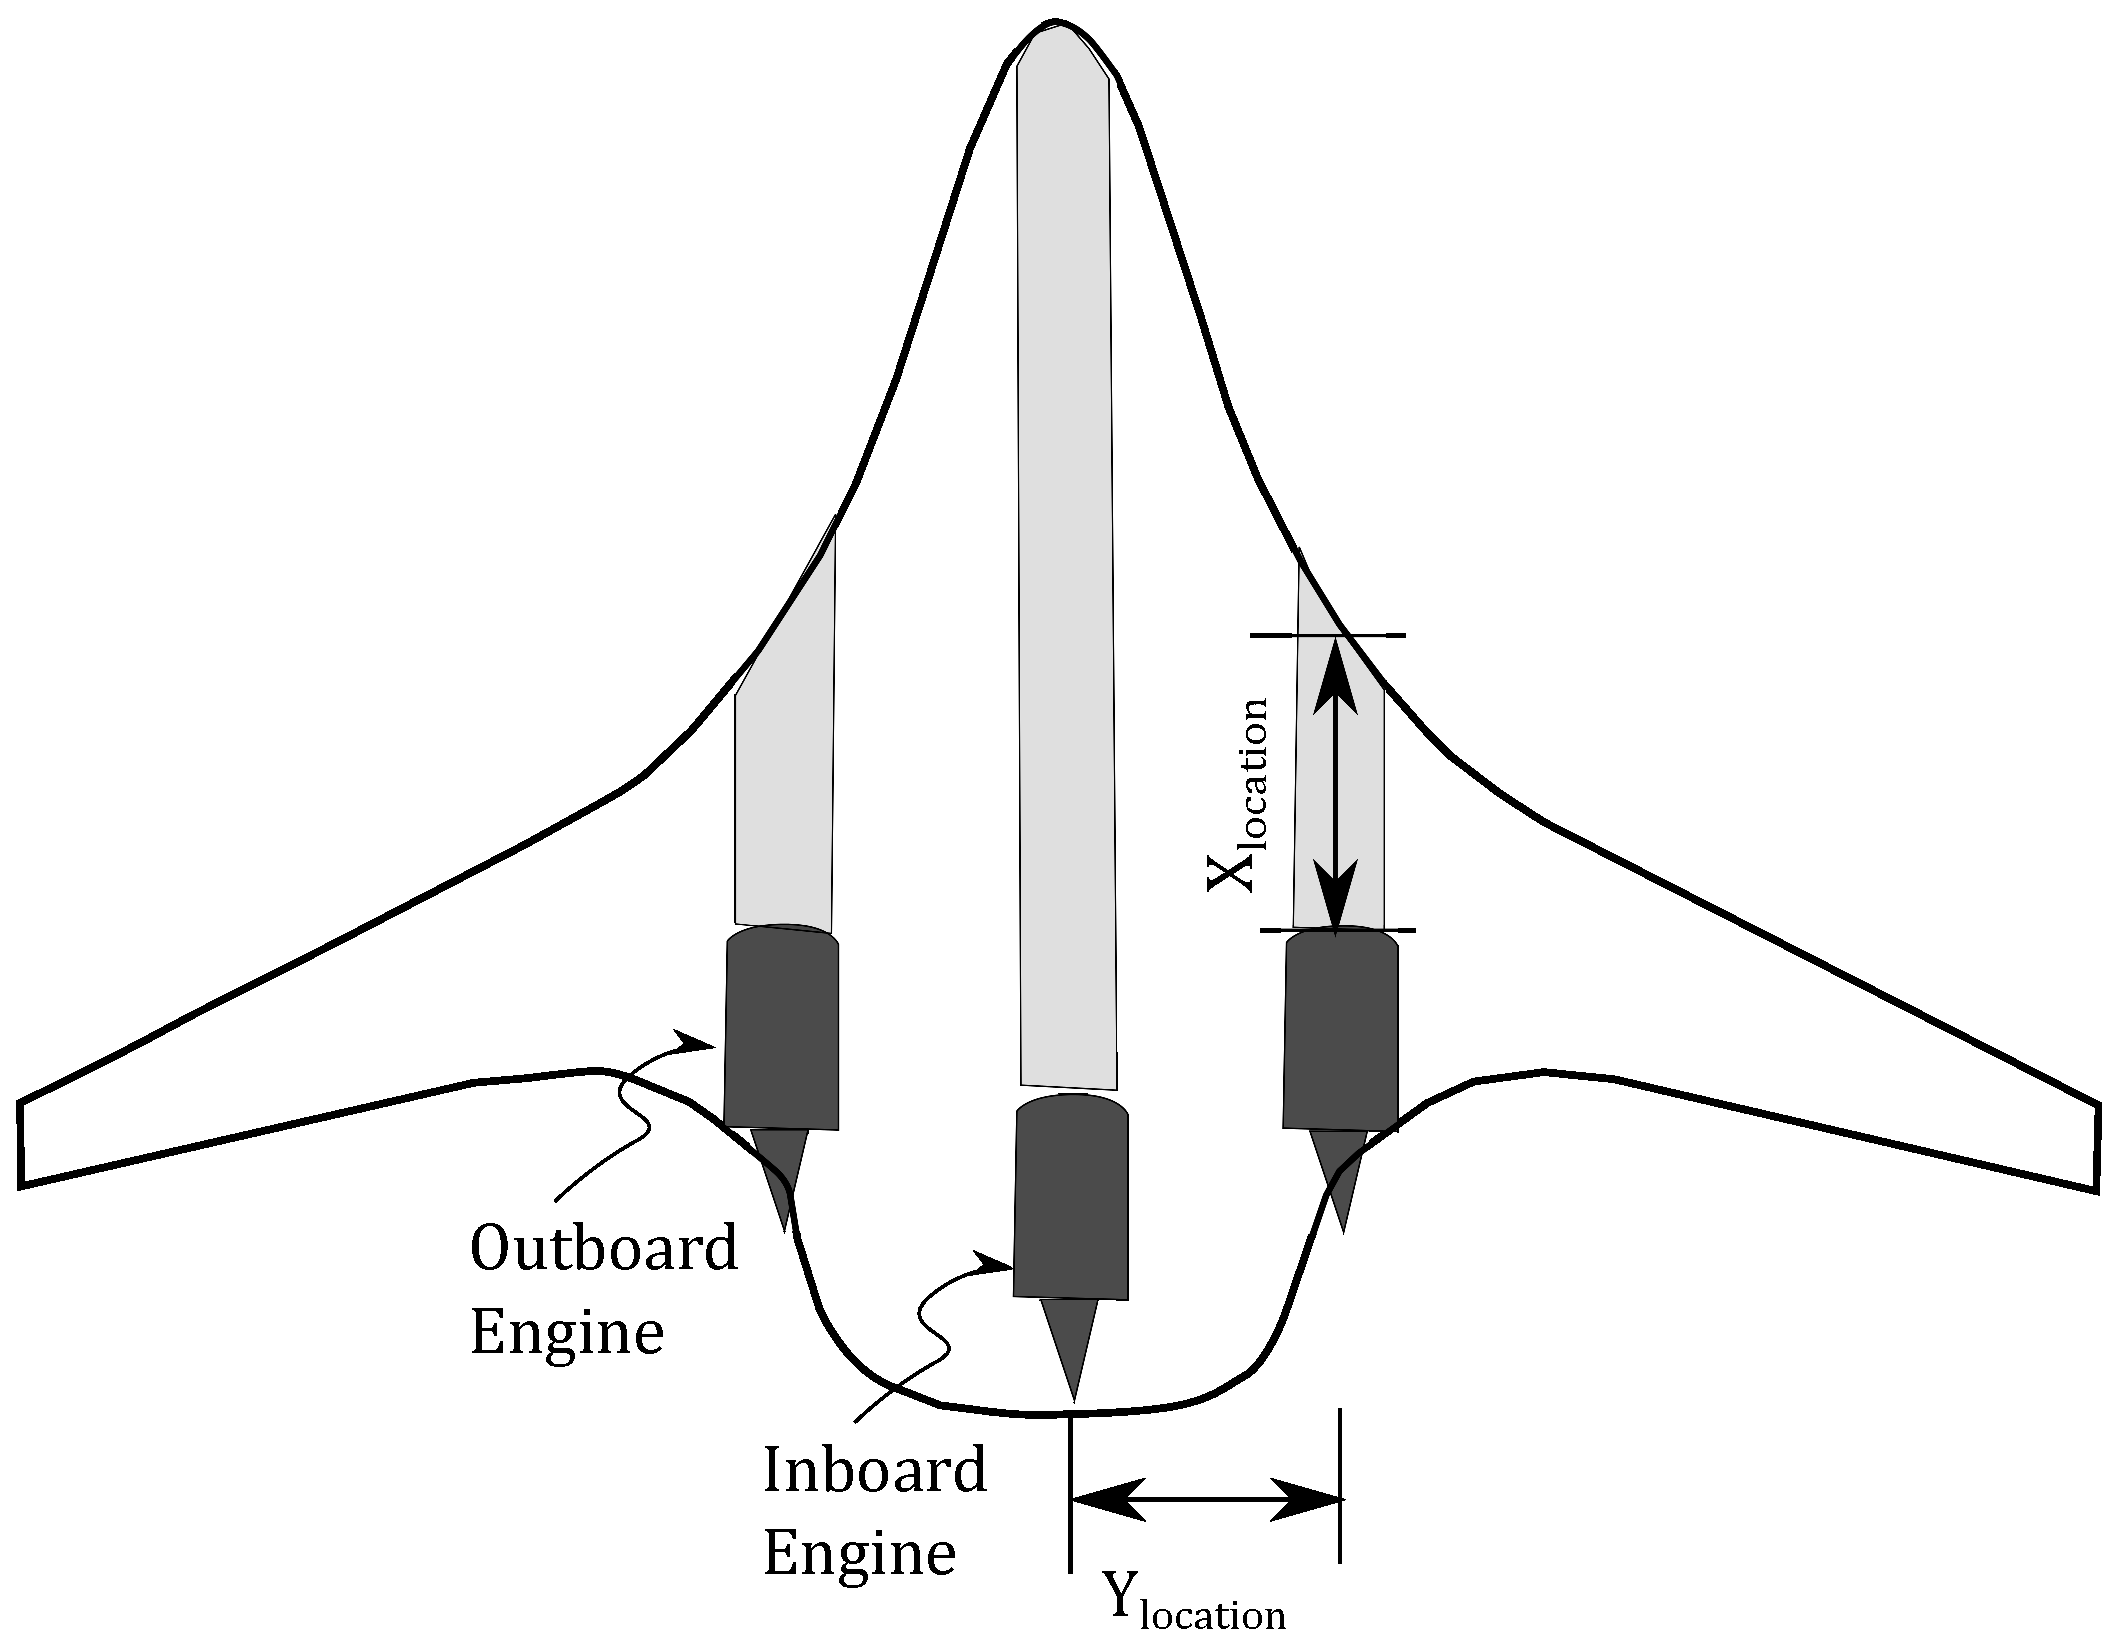
\includegraphics[scale = 0.3, trim = 0mm 0mm 0mm 10mm]{N2A_3_Engine.eps}
				\caption{Illustration of 3-Engine Boeing N2A.}
				\label{N2A_3_Engine}
			\end{figure}		
			\vspace{-10mm}
		\subsubsection{Design Options for 3 Engine HWB}
			The design options for any propulsion system can be specified by showing the design point mapping matrix as defined by Schutte for the MDP process.  Different design potential rules can be specified for each design option.  These are shown in table \ref{N2A_3_Engine_Options}.  The single inlet case is the condition where only the single inlet condition is considered.  This case will be used to test hypothesis 3 and is representative of the standard cycle analysis where only a single propulsor/inlet condition combination is considered.  The single engine is the case where there is only a single design point (one-engine designed).  For this case, there are two options, either inboard core design point or outboard core design point, which raises the question of which is better to choose.  
			\begin{table}[htp, scale = 0.8]
				\renewcommand{\arraystretch}{1.5}% Spread rows out...
				\centering
				\begin{tabular}{ >{\centering}P{3.0cm} | >{\centering}P{2.5cm} >{\centering}P{3cm} >{\centering}P{3cm}  >{\centering \arraybackslash}P{2.cm}}
						   & X = Not used  & D = On-Design      &  O = Off-Design   &  \\
					\hline \hline
					\bf{Design Option} &               & \bf{Core/HP Spool} & \bf{Fan/LP Spool} & \bf{Design Rule} \\
					\hline
						   &   \multicolumn{1}{ >{\centering}P{2.5cm}|}{Inboard}     & D & D &  \\
						   &   \multicolumn{1}{ >{\centering}P{2.5cm}|}{Outboard}     & X & X &  \\
					\cline{2-5}					
		                   &    \multicolumn{1}{ >{\centering}P{2.5cm}|}{Inboard}    & X & X &  \\
					\multirow{-4}{3cm}{Single Inlet} &   \multicolumn{1}{ >{\centering}P{2.5cm}|}{Outboard}    & D & D &  \\
					\hline
		                   &    \multicolumn{1}{ >{\centering}P{2.5cm}|}{Inboard}    & D & D &  \\
		                   &   \multicolumn{1}{ >{\centering}P{2.5cm}|}{Outboard}    & O & O &  \\
					\cline{2-5}					
		                   &    \multicolumn{1}{ >{\centering}P{2.5cm}|}{Inboard}    & O & O &  \\
					\multirow{-4}{3cm}{Single Engine}&   \multicolumn{1}{ >{\centering}P{2.5cm}|}{Outboard}    & D & D &  \\
					\hline
		                   &    \multicolumn{1}{ >{\centering}P{2.5cm}|}{Inboard}    & D & D &  \\
					\multirow{-2}{3cm}{Fixed Core}&   \multicolumn{1}{ >{\centering}P{2.5cm}|}{Outboard}    & O & D &  \\
					\cline{1-5}					
		                   &    \multicolumn{1}{ >{\centering}P{2.5cm}|}{Inboard}    & D & D &  \\				          
					\multirow{-2}{3cm}{Double Engine}&   \multicolumn{1}{ >{\centering}P{2.5cm}|}{Outboard}    & D & D &  \\					                   
					\hline
					\hline
				\end{tabular}
				\caption{Design point mapping matrix for the 3 engine architecture highlighting the available design rules.}
				\label{N2A_3_Engine_Options}
			\end{table}  		
			Finally, there are the two design options where the inboard and outboard propulsors are sized independently.  The fixed core design assumes that only the bypass and LP spool are re-designed for each, while the core/HP spool are designed at either inboard or outboard and held constant.  The double engine is the case where a new engine is sized for both conditions.  In each of these cases, there is a design rule required for the analysis because the size of the propulsors with respect to each other are not fixed.  Therefore, a new variable is defined and called the "mass flow ratio" or MFR, which is not to be confused with the ratio of free-stream tube area to capture which is sometimes called the mass flow ratio.  The MFR is defined as the ratio of the mass flow of the outboard engine to the inboard engine and is considered a cycle parameter.  
			\begin{equation}
				MFR = \frac{\dot{m}_{outboard}}{\dot{m}_{inboard}}
			\end{equation} 
			It is worth noting that other design rules could be used, such as the ratio of the thrusts, which would effectively represent the same thing, but it is easier from a practical standpoint to fix the mass flows of the engine, since mass flow demand is typically an independent parameter while thrust is a dependent result of the cycle analysis.  By using the MFR as the design rule, the mass flow of one engine can be varied to satisfy the thrust matching relation, and the other engine mass flow can be set to a value for each pass through the model based on the MFR.   			
			
			The research question for this section of the thesis pertains to which of the above options is preferable for this application.  Chapter 5 will discuss the modeling setup and implementation of the 3-Engine N2A cycle analysis, as well as the architecture integration phase setup.  From this analysis, general conclusions about choices of design options and design rules for other systems will also be made.  
									 			
  			\vspace{1pt}
  			\vspace{5mm}
  			\noindent{
  				\fbox{
  					\parbox{\textwidth}{
  						\textbf{Research Question 4}:  For BLI propulsion systems, which design options provides the largest benefit?  										 						  			
  					}
  				}
  			}
									
			\subsubsection{Observations and Hypothesis 4} 
				A hypothesis in regard to research question 4 can be made by reiterating the conclusion from :  namely that the performance of the engine changes significantly with the ratio of the boundary layer to inlet height, and that this can be controlled for each propulsor by varying the mass flow ratio.  Having the extra independent mass flow ratio variable allows the designer to match each propulsor to the appropriate boundary layer to height ratio.  However, as discussed previously, there may be countervailing factors that prevent one or more of the propulsors from being sized to a particular level.  
				
				One such potential factor is the existence of significant size effects for gas turbine engines, and specifically the gas turbine core.  To illustrate these effects, \ref{Size_Effects} shows the polytropic efficiency of a high pressure compressor plotted against the exit corrected flow -- a normalized measure of the "size" of the compressor.  Clearly making the gas turbine core very small at its design point by varying the mass flow ratio will have a significant impact on the performance of the core. 
				
				\begin{figure}[htp]
					\centering
					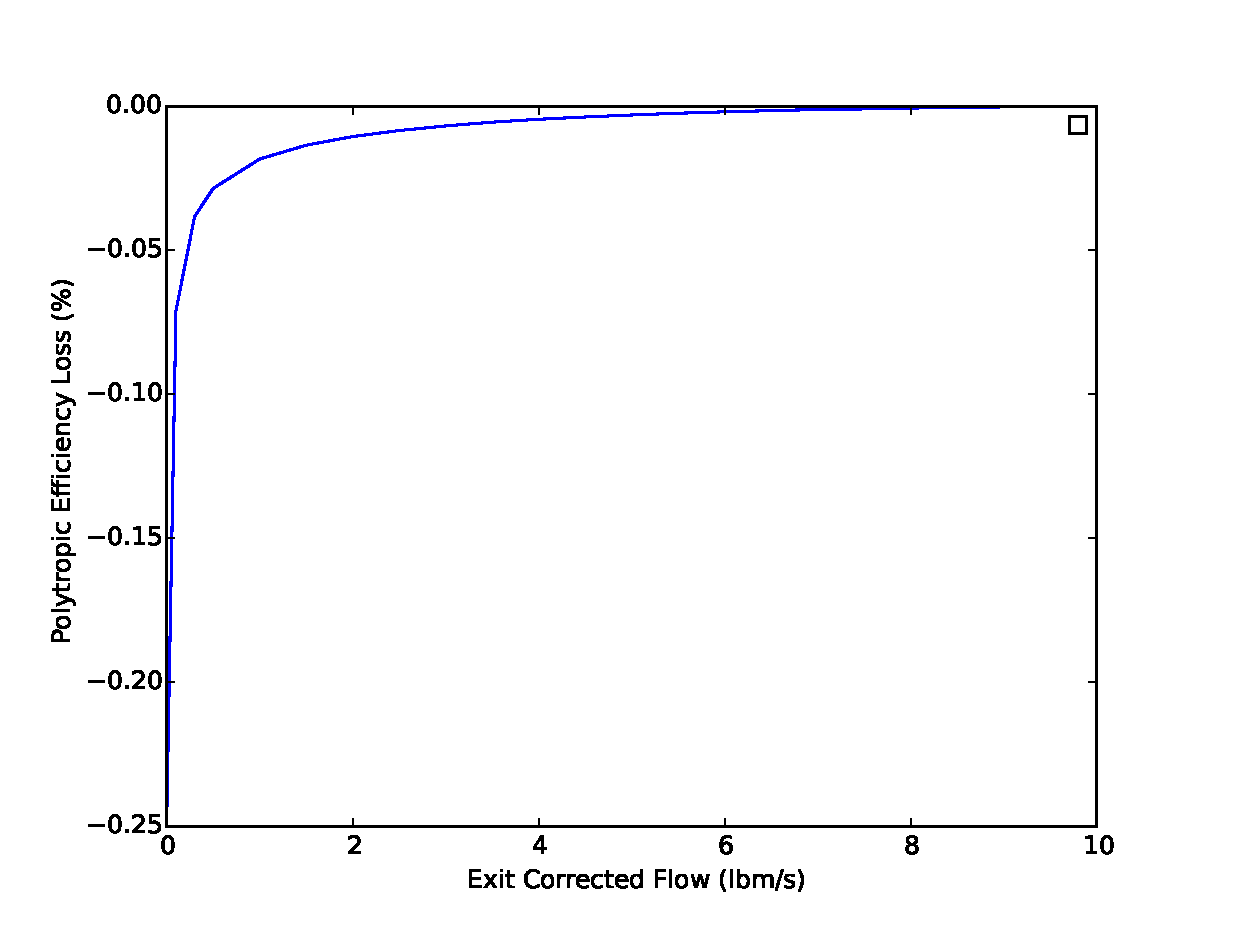
\includegraphics[scale = 0.5]{Size_Effects.eps}
					\caption{Plot showing size effects of a typical gas turbine axial compressor at very small exit corrected flow INSERT REFERENCE HERE.}
					\label{Size_Effects}
				\end{figure}				
				
				Another potential factor which can effect the gas turbine core is flow mis-match which could happen in the case of the fixed core design option.  If the outboard and inboard engines are designed to the same bypass ratio, then the core will need to be "over" or "under" sped in relation to the design point.  This can have a significant impact on the efficiency of the core and the pressure ratio at which it operates.  As such, the following hypothesis is developed based on the above reasoning.  
				
				\noindent\makebox[\linewidth]{\rule{\textwidth}{3pt}}								
				\textbf{Hypothesis 4}:  Sizing a different propulsor for each inlet condition will provide a better fuel burn benefit than the single engine option, unless doing so affects the thermal efficiency of the gas turbine core. As the difference between the engine inlet conditions is increased, so too is the value gained by re-sizing the engine for that inlet condition.
				\noindent\makebox[\linewidth]{\rule{\textwidth}{3pt}}				
					
	\subsection{Vehicle Matching Phase}
		The point of the vehicle matching phase is to determine the flight conditions for which the propulsion system need to be designed and which therefore need to be included in the MDP analysis.  This section will outline the basic requirements for including a flight condition within the MDP analysis, and also outline a method for finding the flight conditions in the most efficient way for a given set of requirements.  Research question five is formulated with respect to this phase of the analysis:

		\vspace{1pt}
		\vspace{5mm}
		\noindent{
			\fbox{
				\parbox{\textwidth}{
				\textbf{Research Question 5:}:  What flight conditions are necessary to include for sizing BLI systems in a MDP cycle analysis?
				}
			}
		}
		
		In general, sizing points need to be included in the MDP analysis if some aspect of the design at that point will  constrain or place more demand on the system.  For instance, it is common to include both top-of-climb (TOC) and take-off (TKO) conditions in an MDP, since TOC places a significant mass flow demand on the system while TKO (especially for a hot day) is the hottest point of operation and therefore sizes the cooling flow which impacts the overall required mass flow and fuel consumption rate.  Looking at the MDP analysis, there are two ways to include flight conditions in the analysis:  constraint points or target points.  For the latter, thrust or cycle targets are precisely met, while constraint points merely constrain some aspect of the system at that point.  For BLI, the thrust or power balance requirement is precisely the same as for a podded system, though the thrust target point may not necessarily be the same as the typical top-of-climb position.  While distortion concerns can be important for podded subsonic inlets, it is not often considered to impact the choice of propulsion system design, but rather impacts the final stall margin stack-up of the fan.  The increased inherent distortion for a BLI system places an additional requirement for a BLI system which must be included in the MDP analysis.
		
		\subsubsection{Thrust Sizing Condition}
			Consider the un-installed thrust of an isolated, ducted fan propulsor:
			\begin{equation}
				T = P_k - \phi_{jet} = \dot{m} \Big(V_j - V_\infty\Big)
			\end{equation}
			Now, define the installation losses of a propulsor in relation to the un-installed thrust value:
			\begin{equation}
				\phi_{inlet} = \frac{F_{loss,_{inlet}}}{T} = \frac{\Phi_{Inlet}}{T \cdot V_\infty}
			\end{equation}
			\begin{equation}
				\phi_{Nozzle} = \frac{F_{loss,_{Nozzle}}}{T} = \frac{\Phi_{Nozzle}}{T \cdot V_\infty}
			\end{equation}			
			The installed net thrust of the propulsor is then:
			\begin{equation}
				F_n = T \cdot (1- \phi_{Nozzle} - \phi_{Inlet}) = \dot{m}\Big(V_j - V_\infty\Big) \cdot (1 - \phi)			
				\label{Installed_Thrust_Equation}
			\end{equation}
			Where $\phi$ is the sum of the inlet and nozzle loss percentages.  For a given fan pressure ratio, increased inlet and fan losses will required a larger propulsor mass flow.  Setting Eq. \ref{Installed_Thrust_Equation} equal to the net thrust required of the vehicle, we get:
			\begin{equation}
				TV_\infty \cdot (1 - \phi) = \Big(DV_\infty + W\dot{h})
			\end{equation}
			and the mass flow required for the engine is then:
			\begin{equation}
				\dot{m} = \frac{D + W\dot{h}/{V_\infty}}{(F_n / \dot{m})(1 - \phi)}
				\label{Max_Mass_Flow}
			\end{equation}
			This can be corrected to sea-level by using the parameter $\delta = P_t/P_{sl}$ and $\theta = T_t/T_{sl}$.			
			\begin{equation}
				\dot{m}_c = \dot{m}\cdot \frac{\sqrt{\theta}}{\delta} = \Big(\frac{D + W\dot{h}/V_\infty}{\delta}\Big)
				\cdot \Big(\frac{1}{1-\phi}\Big) \cdot \Big(\frac{1}{ST_c}\Big)
				\label{mdot_required}
			\end{equation}
			Where $ST_c$ is the corrected specific thrust given by:
			\begin{equation}
				ST_c = \frac{F_n}{\dot{m}\sqrt{\theta}}
			\end{equation}
			
			The corrected specific thrust is mainly a function of the engine/propulsor type, cycle parameter choices, and flight condition.  The general trend of specific corrected thrust for a commercial turbo-fan engine is shown in figure \ref{Lapse_Rates} showing a significant fall at very high Mach numbers such as at the top-of-climb flight condition.
			\begin{figure}[htp]
				\centering
				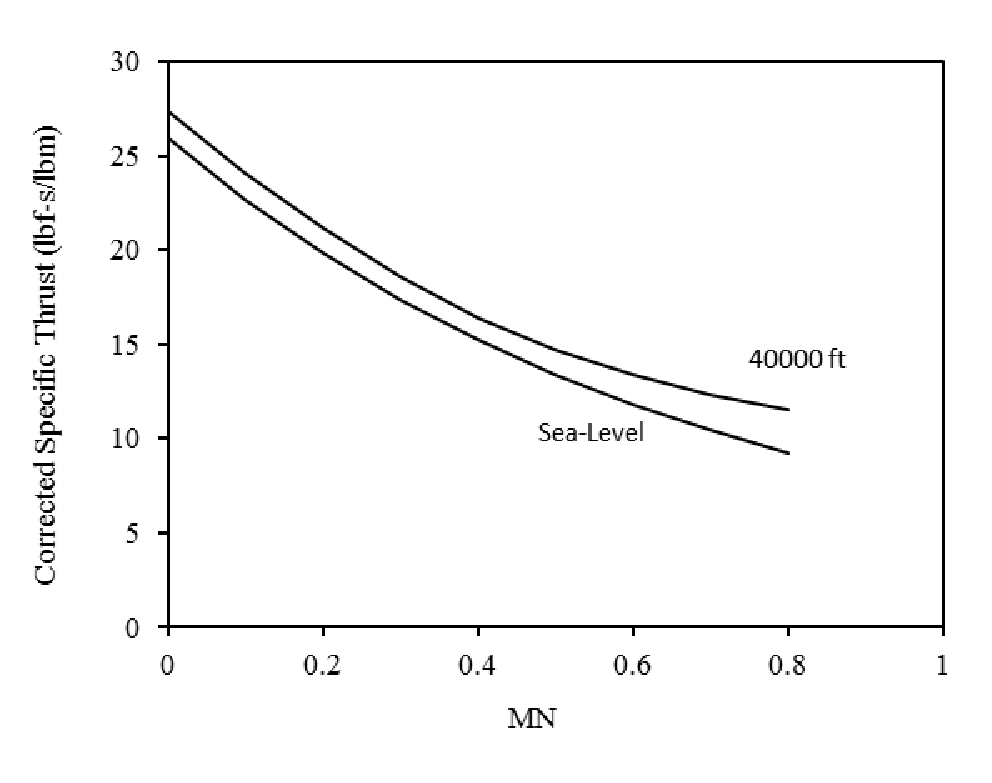
\includegraphics[scale = 0.75]{Lapse_Rates.eps}
				\caption{Turbofan specific thrust vs. Mach number for different altitudes.}
				\label{Lapse_Rates}
			\end{figure}			
			The first term in Eq. \ref{mdot_required} represents the corrected thrust required to power the vehicle.  
			Through the course of the mission of a typical commercial vehicle, the Mach number will obviously increase significantly at cruise flight speeds and the lift coefficient will decline significantly as the weight and lift required is decreased.  The net result is that the corrected thrust required changes over the course of the mission and is generally decreased as the engine moves to top-of-climb.  However, this is not enough to offset the significant decrease in the thrust per unit mass flow delivered at higher flight velocities.  The top of climb condition is therefore typically used to size the mass flow of typical turbofan engines.  
			
			The loss term $\frac{1}{1-\phi}$ can also influence this balance.  If the losses are significant enough at any flight condition, it's possible that this could offset the loss in specific corrected thrust in the final term.  
			
		\subsubsection{BLI Case}
			For BLI, the primary difference is that there is now a benefit term represented by the thrust saving coefficient, as derived previously.  
			\begin{equation}
				F_n = T \frac{(1-\phi)}{1-TSC}
			\end{equation}
			From the previous analysis, Eq. \ref{mdot_required} can be updated to include the thrust saving coefficient due to the boundary layer ingestion.
			\begin{equation}
				\dot{m}_o = 
				\Big(\frac{D + W\dot{h}/V_\infty}{\delta}\Big)
				\cdot \Big(\frac{1-TSC}{1-\phi}\Big) \cdot \Big(\frac{1}{ST_c}\Big)
				\label{BLI_mdot_required}
			\end{equation}										
			This means that the critical flight condition may potentially change depending on the ratio of the boundary layer benefit to losses represented by the second term of Eq. \ref{BLI_mdot_required}.  It also potentially means that the critical mass flow sizing condition could be dependent the amount of boundary layer ingested, which was seen previously to have a significant impact on the system TSC and losses.  
			
			Futhermore, this shows that the BLI engine will have a fundamentally different lapse profile with respect to a podded engine to the change in the amount of wake recovery that occurs as the Mach and Reynolds number is changed during the flight.  This could potentially have an impact on the optimal flight path that the vehicle might take, implying that a much tighter coupling between vehicle and propulsion system designers must take place for commercial BLI systems which ingest significant amounts of boundary layer.
			
		\subsubsection{Stall Margin Condition}			
			Consider a fan operating at some pressure ratio (PR) and corrected flow $(W_c = W \cdot \dfrac{\sqrt{\theta}}{\delta})$ and exhaust area $A_e$.  As the ambient conditions and throttle change, the area must necessarily remain constant.  Given this, Eq. \ref{Nozzle_Exit_Area} shows a relationship between the constant area, the ambient conditions, and the nozzle exit velocity.
			\begin{equation}
				A_e = constant = \frac{W}{\rho_e u_e} = W \cdot \dfrac{\sqrt{\theta}}{\delta} \cdot \frac{1}{M_e}
				\label{Nozzle_Exit_Area}
			\end{equation} 
			From Mattingly INSERT REFERENCE HERE, the equation for the fan exhaust stream is given by:
			\begin{equation}
				M_e = \sqrt{\frac{2}{\gamma-1}\Big(\pi_r \pi_d \pi_f \pi_{fn} - 1.0\Big)}
				\label{Fan_Nozzle_Exit_Mach}
			\end{equation}
			Where $\pi_d$ is the diffuser pressure recovery, $\pi_f$ is the fan pressure ratio (a.k.a FPR), $\pi_{fn}$ is the fan nozzle duct pressure drop, $\pi_r$ is the ram recovery term given in Eq. \ref{Ram_Recovery}, and $\gamma$ is the ratio of specific heats.
			\begin{equation}
				\pi_r = \Big(1 + \frac{\gamma-1}{2}M_o^2\Big)^{\dfrac{\gamma}{\gamma-1}}
				\label{Ram_Recovery}
			\end{equation}
			Clearly, two factors are of major importance in determining the flow required for a given nozzle exhaust area, which are the fan operating pressure ratio and the flight Mach number.  At hot day TKO, the flight Mach number is substantially reduced relative to cruise or TOC, and the nozzle becomes unchoked  ($M_e < 1$).  This forces a decrease in flow (and therefore RPM) for a fixed fan pressure ratio.  For a fixed corrected speed ($N/\sqrt{\theta}$), there is an increase in pressure ratio and decrease in flow.  This necessarily moves the fan closer to the stall line.  
			
			The other major factor is the design pressure ratio of the fan, which substantially increases the BPR of the engine -- something typically desirable for efficiency.  From Eq. \ref{Fan_Nozzle_Exit_Mach}, the Mach number at the nozzle exit will decline significantly for lower $\pi_f$ (higher BPR).  The impact of both flight condition and choice of engine BPR for a typical turbofan engine is shown in figure \ref{Stall_Trends}, where the operating line at hot day TKO and higher bypass ratio is much more stall critical.
			\begin{figure}[htp]
				\centering
				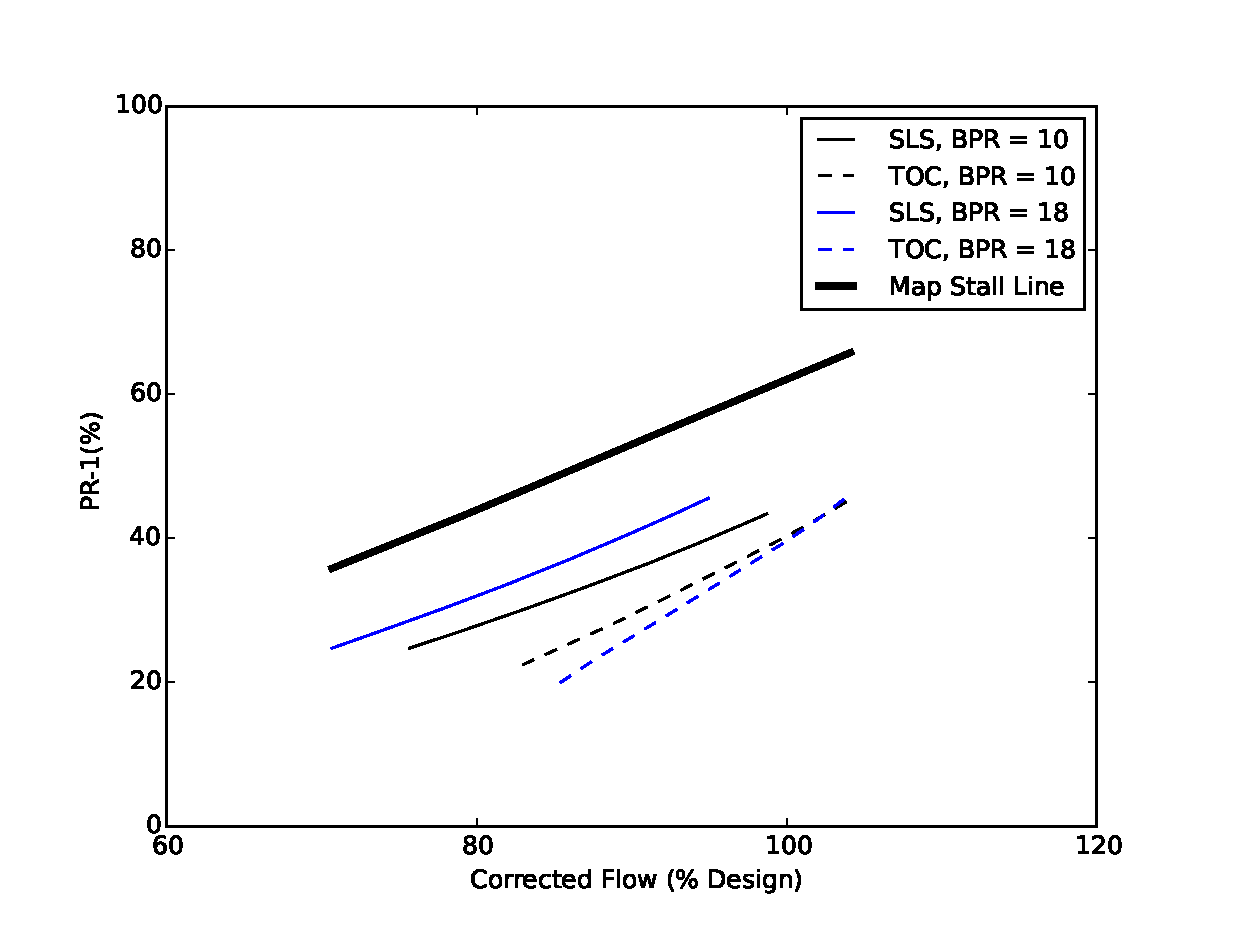
\includegraphics[scale = 0.7]{Stall_Trends.eps}
				\caption{Commercial turbofan variation in fan operating line with flight condition.  Trends show that SLS hot day is critical and is worse at higher BPR.}
				\label{Stall_Trends}
			\end{figure}
			
			\subsubsection{BLI Case}
				For BLI, the limiting stall condition will be that flight point where the fan operating line moves closest to the stability line after modification from the BLI related distortion.  If any point is predicted to have a lacking stability margin after distortion is accounted for, then additional margin must be added to compensate.  This must be done by either mitigating the effects of the distortion on the system or by modifying the fan exhaust area to move the operating line farther from the stability limit.  
				
				So, while the basic trend for a turbofan engine is that stall is generally much more critical at sea-level TKO conditions, the increased distortion at higher Mach numbers could make flight speeds at high power more critical.  Conditions which require very high angles of attack should also be considered such as take-off and landing where large amounts of lift is required and the engines are generally at worse stall margin anyway.  Cycle choices, such as the fan pressure and bypass ratios, will have also a significant impact on both the stall margin variation over the flight envelope, the amount of distortion ingested, and the stall margin loss due to distortion.  As such, one major claim of this thesis is that the most critical stall condition for a given vehicle and requirements set cannot necessarily be assumed known prior to conducting the analysis.  The following section discusses the potential ways this problem might be dealt with and discusses the reasoning for choosing the method implemented in the BLIPSS methodology.  
				
		\subsubsection{Options for Determining Flight Conditions}
			The analysis from the previous sections showed that both the thrust target point and stall margin (distortion) constraint point for a BLI system might vary significantly depending on the choice of cycle design, the level of boundary layer ingested, and the flight requirements imposed on the system.  
			\begin{figure}[htp]
				\centering
				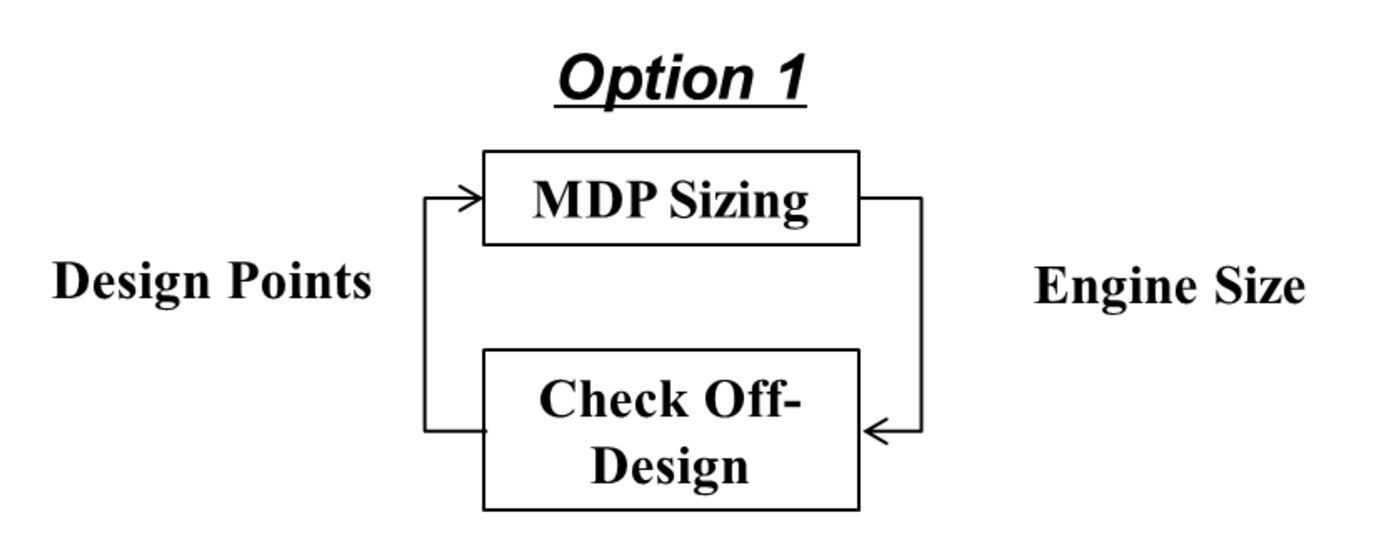
\includegraphics[scale = 0.5]{Vehicle_Matching_Option_1.eps}
				\caption{Option 1 of 3 for determining the flight conditions where all off-design conditions are checked and iterated with the MDP sizing procedure.}
				\label{Vehicle_Matching_Option_1}
			\end{figure}	
			One option for finding these conditions would be to check every single off-design flight condition within the mission flight envelope -- illustrated in figure \ref{Vehicle_Matching_Option_1}.  The problem with this is that it violates the purpose of the MDP methodology to begin with:  to reduce the amount of design iterations needed to converge on the required engine size.  Depending on the complexity of the cycle model, it may take many iterations and off-design cycle analysis runs to finish this process.  
			
			The second option for determining the flight conditions would be to include every condition in the multi-design point process as in figure \ref{Vehicle_Matching_Option_2}.  Given that there may be many conditions to check if the entire mission envelope is included, this would place an unmanageable level of program complexity on the cycle designer and may have convergence issues if a single initial iterate is used.  
			\begin{figure}[htp]
				\centering
				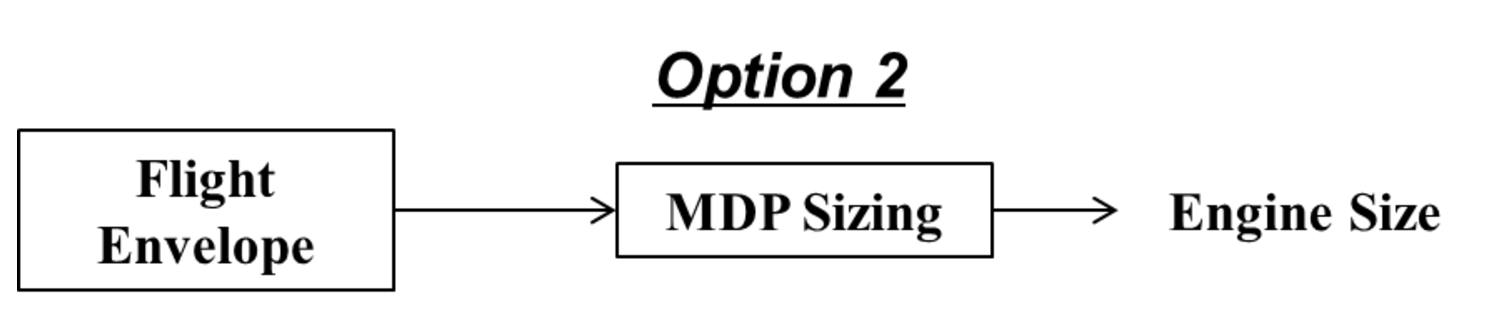
\includegraphics[scale = 0.5]{Vehicle_Matching_Option_2.eps}
				\caption{Option 2 of 3 for determining the flight conditions where all off-design conditions are included as constraint points within the MDP.}
				\label{Vehicle_Matching_Option_2}
			\end{figure}	
			The final option, as illustrated in figure \ref{Vehicle_Matching_Option_3}, is to assume that some subset of the total flight condition set will cover the majority of the critical conditions over the span of the design space.  The process will then setup a screening design of experiments which represents a range of the design space to determine the likely critical flight conditions.   
			\begin{figure}[htp, trim = 25mm 0mm 0mm 0mm]
				\centering
				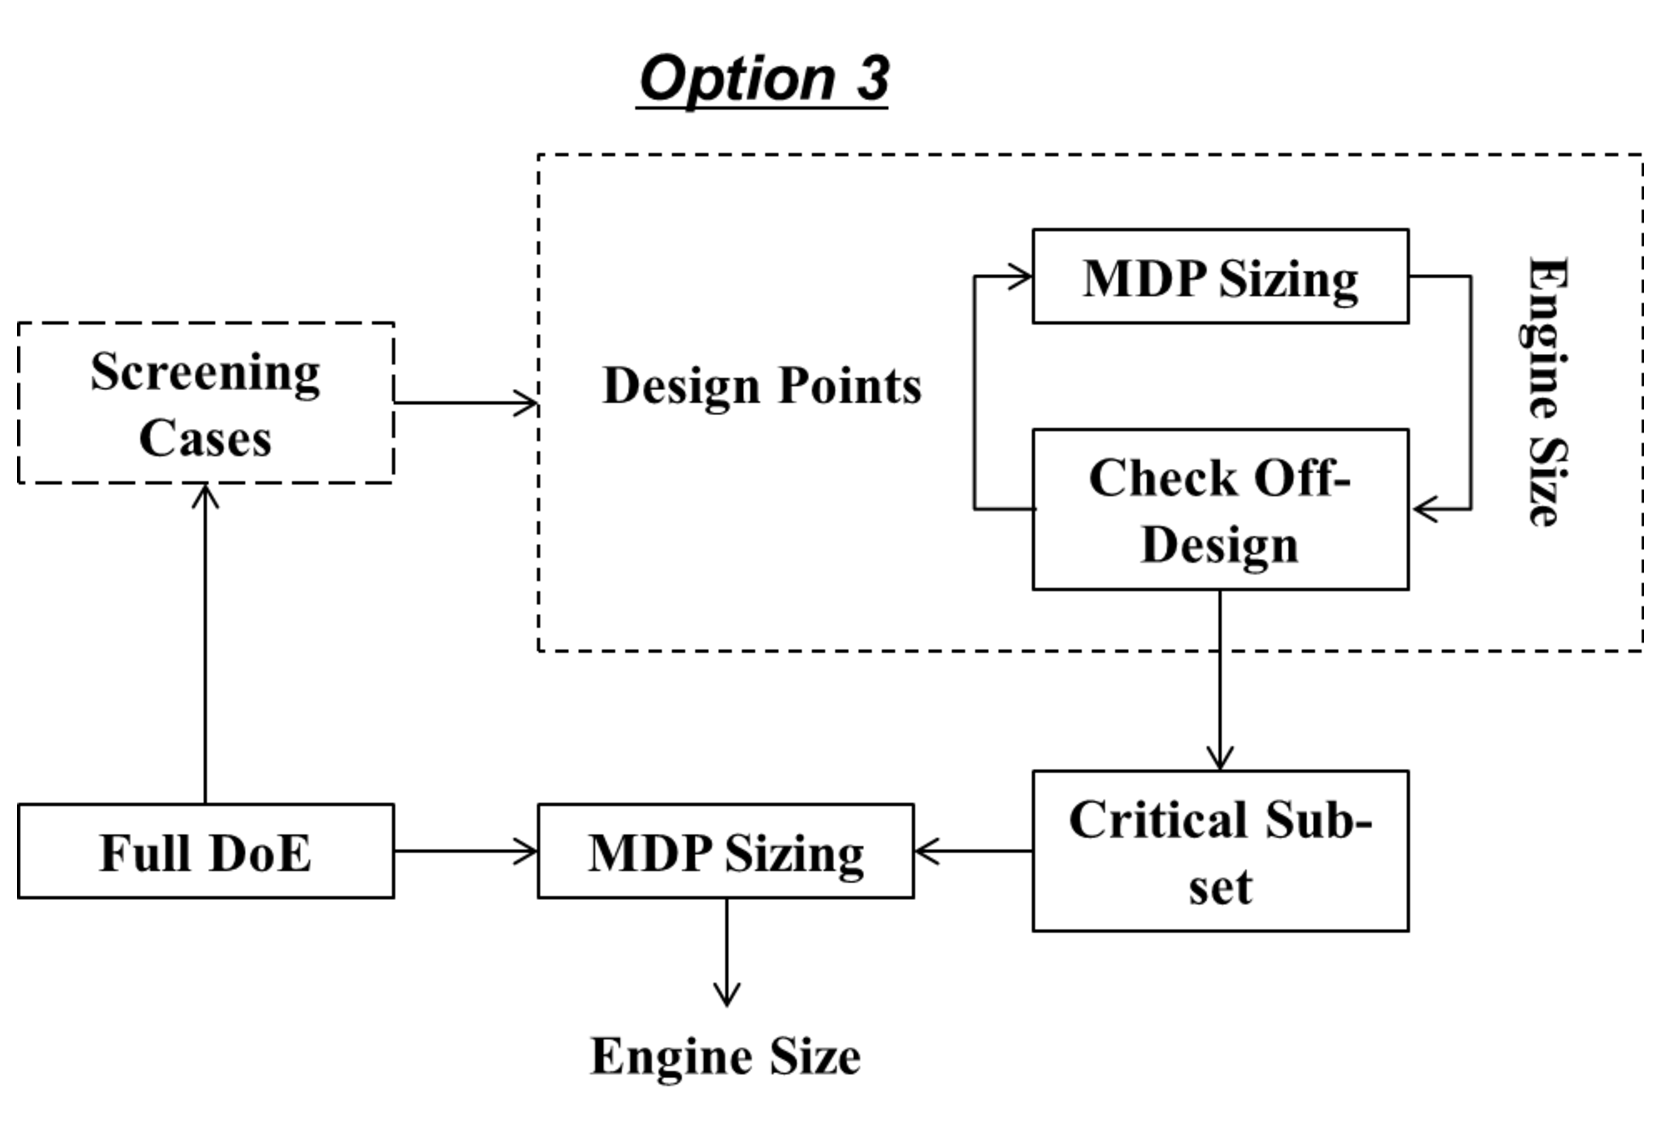
\includegraphics[scale = 0.5]{Vehicle_Matching_Option_3.eps}
				\caption{Option 3 of 3 for determining the flight conditions where a subset of critical conditions are identified using a screening design of experiments; all subsequent cases do not run off-design iteration checks.}
				\label{Vehicle_Matching_Option_3}
			\end{figure}	
			
			For screening cases, the first option is implemented and all off-design conditions are checked.  For non-screening cases, off-design is not checked, and only the MDP sizing procedure is run.  The final selected design can then also be run through the off-design check to ensure that it's critical sizing conditions were appropriate and that no off-design conditions have thrust or stall margin deficits. 
			
			Obviously option 3 is the one that seems most viable given the above analysis and is therefore implemented in the BLIPSS methodology algorithm description in figure \ref{Design_Methodology}.  To verify that this process is acceptable, the following hypothesis is made and will be tested thoroughly in chapter 6 with a numerical simulation and experiment on the canonical BLI problem. 
			
			\noindent\makebox[\linewidth]{\rule{\textwidth}{3pt}}				
			\textbf{Hypothesis 5:}:  Off-design flight conditions for BLI should be included as constraint points in the MDP requirements setup phase if thrust or stall margin loss due to BLI installation effects, which were not present in the podded case, become sufficiently high such that a larger engine size or additional design stall margin is required to accommodate the thrust and stability requirements at that flight condition.  A small subset of all possible flight conditions can be found, for a given propulsion system architecture and requirements set, which captures the most critical conditions for a large majority of designs in the design space. \\
			\noindent\makebox[\linewidth]{\rule{\textwidth}{3pt}}				